\documentclass[11pt]{article}
\usepackage{amsmath}
\usepackage{amssymb}
\usepackage[T1]{fontenc}
\usepackage{booktabs}
\usepackage{graphicx}
\usepackage{xcolor}
\usepackage[margin=1in]{geometry}
\usepackage[square,numbers,sort&compress]{natbib}
\usepackage{array}
\newcolumntype{H}{@{}>{\setbox0=\hbox\bgroup}c<{\egroup}@{}}
\usepackage{adjustbox}
\usepackage[section]{placeins}
\usepackage{hyperref}
\hypersetup{colorlinks=true, linkcolor={blue!55!black}, citecolor={green!35!black}, urlcolor={blue!55!black}}
\makeatletter\setlength{\@fptop}{0pt}\setlength{\@fpsep}{14pt plus 2fil}\setlength{\@fpbot}{0pt plus 1fil}\makeatother
\setlength{\parskip}{0.35em}
\setlength{\parindent}{0pt}
\newcommand{\nzo}{\mathcal{N}(0,1)}
\newcommand{\code}[1]{\texttt{#1}}
\makeatletter\newcommand{\inputrows}[1]{\@@input #1 }\makeatother
\makeatletter\newcommand{\runinsubsection}{\@startsection{subsection}{2}{\z@}{3.25ex \@plus1ex \@minus.2ex}{-1em}{\normalfont\normalsize\bfseries}}\makeatother
\newenvironment{plan}{\par\color{gray}\small\textbf{Plan.}\ }{\par}
\newcommand{\tbd}{{\color{red}[insert here]}}
\newcommand{\secTBD}{{\color{red}*}}
\newcommand{\threecols}{ & $n=50$ & $n=100$ & $n=10{,}000$ \\}
\newcommand{\pc}[2]{\begin{tabular}[c]{@{}c@{}}#1\\[-2pt]{\scriptsize #2}\end{tabular}}  % paired-test cell (Appendix tables)   % section number to fill in once Results is revised (2026-11-05)
\newcommand{\repro}[1]{\par{\raggedright\color{gray}\footnotesize\textbf{Reproduce:} #1\par}}

\begin{document}
\sloppy

\begin{center}
{\Large\bfseries Bayesian neural networks versus neural posterior estimation\\
for simulation-based inference with little data}\\[0.5em]
{\normalsize Sam Dowd}\\[0.2em]
{\small Seljak Group, UC Berkeley}\\[0.2em]
{\small November 2026}
\end{center}

\begin{abstract}
We construct a toy problem for simulation-based inference (SBI) on cosmological fields, which in the simplest,
Gaussian setting depend on their parameters only through the power spectrum: inferring the amplitude and length scale
of a radial basis function (RBF) kernel, which set a Gaussian field's power spectrum, from the empirical covariance of
ten noisy draws of the field, a task whose exact posterior is known. On it we compare Bayesian neural networks (BNNs)
sampled with Microcanonical Langevin Ensembles (MILE) against neural posterior estimation (NPE) at small simulation
budgets, $n=50$ to $10{,}000$. Three 12-chain BNNs, under MILE's default $\mathcal N(0,1)$ prior, with a weight-prior
scale chosen without training data (the data-free prior) and with a tempered likelihood, are compared with 12-member
ensembles of NPE and of the BNN's own networks trained without sampling. Against single networks the BNN has the lower
test negative log-likelihood (NLL) at every $n$, but at $n\le100$ ensembling the baselines matches this advantage.
Against ensembles, the BNN does not beat NPE on average in the low-data regime: NPE is better at $n=100$ by
0.18--0.29 nats, and at $n=50$ only the BNN with the data-free prior is marginally better. The BNN beats NPE from
$n=500$ with tempering and from $n=5{,}000$ without, by 0.11--0.20 nats. At small $n$ the BNN is nonetheless the more
reliable estimator: its test NLL varies 3--6 times less across training sets than NPE's, its worst training set is
better, and it is never badly over-confident, which we argue matters more than the average when one estimator is
trained once and applied to one observation. Under $\mathcal N(0,1)$ the BNN is too wide at small $n$, almost entirely
in its aleatoric term; against the exact posterior this is not irreducible noise, and we read it as epistemic
uncertainty from a misspecified prior reported as aleatoric. The data-free prior removes most of the excess and helps
most at the smallest $n$, where the scale of the prior is the dominant error; tempering helps most at intermediate
$n$, where what remains is the isotropic Gaussian form of the prior.
\end{abstract}

\tableofcontents

\section{Introduction}
\label{sec:intro}
Many sciences describe phenomena with simulators whose likelihood is intractable but from which data are easy to draw
\citep{cranmer2020frontier}. Simulation-based inference (SBI) turns this around and learns the map from data back to
parameters from simulated pairs. In neural posterior estimation (NPE), its most widely used form, a conditional density
estimator, typically a normalizing flow, is trained on pairs $(\theta,x)$ to approximate the posterior directly
\citep{papamakarios2016fast,papamakarios2017maf}. Cosmology is one of the fields where this matters most. In the
simplest, Gaussian setting a cosmological field depends on its parameters only through its power spectrum
\citep{makinen2021lossless}, and realistic field simulations are expensive enough that training sets are often small.
Even CAMELS (Cosmology and Astrophysics with Machine Learning Simulations), the largest suite of cosmological
hydrodynamic simulations built for training machine-learning models, contains only a few thousand simulations
\citep{villaescusa2021camels}.

Small training sets raise a problem that NPE does not address. An estimator that has seen few simulations is itself
uncertain about the inverse map, and that uncertainty ought to widen the posterior it reports. A standard NPE has no
way to express it, since it returns a single fitted density whatever the budget, and neural SBI algorithms are known to
produce over-confident posteriors \citep{hermans2022trust}. In scientific use this is the more harmful kind of error,
because an over-confident posterior excludes parameter values that the data do not rule out. Ensembling several
estimators is one remedy, and \citet{hermans2022trust} recommend it.

Bayesian neural networks (BNNs) offer a more direct one. By placing a posterior over the network's weights, a BNN adds
to its predictive an epistemic term, the uncertainty about the network itself, which should be large when the training
set is small and shrink as it grows \citep{kendall2017uncertainties}. Two recent studies have compared BNNs with NPE.
\citet{delaunoy2024lowbudget} make the NPE flow itself Bayesian and find it conservative down to very small budgets,
where NPE is over-confident, although it becomes accurate more slowly than NPE as the budget grows.
\citet{poh2025lensing}, working with several hundred thousand simulations, find NPE more accurate and better calibrated
than their BNN, which is under-confident. In both studies the BNN is fitted by variational inference, and neither
compares the results with a reference posterior. It therefore remains open how a BNN whose posterior is sampled rather
than approximated would fare against NPE, and how close either comes to the true posterior.

Sampling BNN posteriors by Markov chain Monte Carlo (MCMC) has long been considered impractical, because posteriors
over network weights are high-dimensional and multimodal \citep{papamarkou2022challenges,izmailov2021bnn}.
Microcanonical Langevin Ensembles (MILE) have recently made it practical at moderate cost \citep{sommer2025mile}. MILE
first trains a deep ensemble, a set of independently trained networks, and then starts a short Microcanonical Langevin
Monte Carlo (MCLMC) chain \citep{robnik2024mclmc} from each member. This construction affects how a MILE BNN should be
evaluated. Deep ensembles, which average the predictions of their members, are themselves the standard non-Bayesian
way to obtain epistemic uncertainty, and they can be read as an approximation to Bayesian model averaging
\citep{lakshminarayanan2017ensembles,wilson2020bayesian}. A MILE BNN is therefore both an ensemble and a sampler, and
comparing it with a single network credits sampling with improvements that ensembling alone would provide. To isolate
what sampling contributes, the baselines have to be ensembled to the same size, and the comparison needs a control made
of the BNN's own networks without sampling.

\paragraph{Question.} \emph{Do BNNs sampled with MILE perform better than NPE when the simulation budget is small?}
We study this question on a toy version of cosmological field inference for which the exact posterior is available
(Section~\ref{sec:why_task}). The task is to infer the amplitude and length scale of a radial basis function (RBF)
kernel, which together set the power spectrum of a Gaussian field, from the empirical covariance of ten noisy draws of
the field. We train three methods on 50 to 10{,}000 simulations, each as a 12-member ensemble. The first is a BNN
sampled with MILE, the second is NPE, and the third is a Gaussian predictor, which consists of the BNN's own networks
trained to convergence and not sampled. Comparing the BNN with the Gaussian predictor isolates what sampling adds, and
comparing it with NPE compares the two approaches at equal ensemble size. All methods are scored mainly by the test
negative log-likelihood (NLL) of the true parameter, which does not require the posterior. We use the exact posterior
in the appendices to check each method's mean, width and calibration, and to examine how the BNN divides its
uncertainty into aleatoric (irreducible) and epistemic parts.

\paragraph{Contributions.} Our first contribution is the comparison itself, in which every method is ensembled to the
same size so that the effects of ensembling and of sampling can be told apart. Against a single network the BNN is
better at every budget, but at small budgets ensembling the baselines removes most of that advantage
(Sections~\ref{sec:res_single} and~\ref{sec:res_ens}). Second, we find that at small budgets the BNN does not beat an
NPE ensemble on average, but it is the more reliable estimator. Its test NLL varies several times less from one
training set to the next, and it is never badly over-confident. We argue that this reliability is what matters when an
estimator is trained once and applied to a single observation (Section~\ref{sec:disc_answer}). At large budgets the
BNN also wins on average, which is the opposite of what has been reported for variational BNNs. Third, under MILE's
default prior the BNN is too wide at small budgets, and almost all of the excess lies in its aleatoric term. The exact
posterior shows that this extra width is not irreducible noise, and we interpret it as epistemic uncertainty, caused by
a misspecified prior, that the network reports as aleatoric (Sections~\ref{sec:variants}
and~\ref{sec:disc_aleatoric}). Finally, the scale and the form of the prior matter at different budgets. A prior scale
chosen without training data removes most of the excess width and helps most at the smallest budgets, while tempering
the likelihood helps most at intermediate ones. This pattern is consistent with a prior whose scale can be set
correctly but whose isotropic Gaussian form is misspecified (Section~\ref{sec:disc_adjust}).

\section{Background}
\label{sec:background}

\subsection{Simulation-based inference and neural posterior estimation}
\label{sec:bg_sbi}
A simulator defines a prior $p(\theta)$ and a way to draw data $x\sim p(x\mid\theta)$ whose density is
intractable; the goal is the posterior $p(\theta\mid x)\propto p(x\mid\theta)\,p(\theta)$ for an observed $x$
\citep{cranmer2020frontier}. Neural posterior estimation \citep{papamakarios2016fast} fits a conditional density
$q_\phi(\theta\mid x)$ to simulated pairs $(\theta_i,x_i)\sim p(\theta)\,p(x\mid\theta)$ by maximizing
$\sum_i\log q_\phi(\theta_i\mid x_i)$. In expectation this objective equals the negative
expected Kullback--Leibler (KL) divergence $-\mathbb{E}_{p(x)}\,\mathrm{KL}\big(p(\theta\mid x)\,\|\,q_\phi(\theta\mid x)\big)$ up to a constant, so a
sufficiently flexible $q_\phi$ recovers the posterior, for every $x$ at once (amortization). The usual family is a
normalizing flow, e.g.\ a masked autoregressive flow, ``a stack of autoregressive models, each modelling the
random numbers of the next'' \citep{papamakarios2017maf}.

With a finite budget the objective is a sample average over $n$ pairs, and the fitted $\phi$ carries no
uncertainty of its own: the estimator reports a single density whatever $n$ is. Neural SBI algorithms ``can yield
overconfident posterior approximations'', and ensembles of estimators are more reliable
\citep{hermans2022trust}. Evaluation matters as much as the algorithm, since ``the choice of performance metric is
critical'' \citep{lueckmann2021benchmark}. Without the true posterior, calibration is tested from samples:
simulation-based calibration (SBC) checks the ranks of true parameters among posterior draws \citep{talts2018sbc}, and
TARP (Tests of Accuracy with Random Points) is a coverage test that is necessary and sufficient for an accurate
estimator \citep{lemos2023tarp}. Here the true posterior is available (Section~\ref{sec:reference}). The main
comparison does not need it, since the test NLL uses only the true parameter; the appendices use it to compare each
estimator's moments, width and calibration with the posterior directly.

\subsection{Bayesian neural networks and deep ensembles}
\label{sec:bg_bnn}
A BNN places a prior $p(\mathbf w)$ on the weights of a network defining $p(y\mid x,\mathbf w)$, and predicts with
the posterior predictive
\begin{equation}
p(y\mid x,\mathcal{D})=\int p(y\mid x,\mathbf w)\,p(\mathbf w\mid\mathcal{D})\,\mathrm{d}\mathbf w,\qquad
p(\mathbf w\mid\mathcal{D})\propto p(\mathcal{D}\mid\mathbf w)\,p(\mathbf w)
\end{equation}
\citep{neal1996bayesian,mackay1992practical}. With a heteroskedastic likelihood, one whose predicted
width depends on the input, the predictive variance splits into an aleatoric part, the expected predicted noise, and an
epistemic part, the spread of the predicted means over the posterior (Eq.~\eqref{eq:decomp}); how the BNN's split behaves on this task is examined in
Appendix~\ref{app:width}.

A non-Bayesian alternative is the deep ensemble: independently trained networks averaged at prediction, which is
``simple to implement, readily parallelizable'' and gives ``well-calibrated uncertainty estimates which are as good
or better than approximate Bayesian NNs'' \citep{lakshminarayanan2017ensembles}; deep ensembles also ``provide an
effective mechanism for approximate Bayesian marginalization'' \citep{wilson2020bayesian}. MILE starts its chains from a deep
ensemble (Section~\ref{sec:mile}), and the baselines are also run as ensembles to separate the effect of sampling
from that of ensembling.

\subsection{Sampling BNN posteriors with MILE}
\label{sec:bg_sampling}
\label{sec:mile}
MCMC targets $p(\mathbf w\mid\mathcal{D})$ exactly in the limit, but BNN posteriors are
high-dimensional, multimodal and non-identifiable: permuting hidden units or rescaling between layers leaves the
function unchanged. \citet{papamarkou2022challenges} trace the resulting obstacles to a ``lack of convergence to the
parameter posterior'', yet show that a non-converged chain ``can yield via Bayesian marginalization a valuable posterior
predictive distribution''. Full-batch Hamiltonian Monte Carlo (HMC) chains \citep{izmailov2021bnn} disagree in weight space but mostly agree in
function space, and \citet{sommer2024connecting} propose Bayesian deep ensembles, chains initialized at the members of a
deep ensemble, since ``multiple samples from multiple chains improve predictive performance and uncertainty
quantification''. Cost is the other obstacle: the No-U-Turn Sampler (NUTS),
the adaptive form of HMC, ``often requires more than 90k leapfrog steps/gradient evaluations for
warmup in BNN tasks'' \citep{sommer2025mile}.

MCLMC \citep{robnik2024mclmc} samples with a unit-speed velocity whose dynamics leave the target invariant for any noise
level. It is integrated with a step size $\epsilon$, the velocity is partially refreshed over a decoherence length $L$,
and there is no Metropolis--Hastings correction, so a finite $\epsilon$ biases the stationary distribution; the bias is
controlled by tuning $\epsilon$ to a target energy-error variance per dimension (EEVPD; Appendix~\ref{app:bg}).
MILE \citep{sommer2025mile} (Figure~\ref{fig:mile}) turns MCLMC into a sampler for BNN posteriors. It decomposes the
error of the Monte Carlo predictive
\begin{equation}
\label{eq:mc_predictive}
p(\mathbf{y}^\ast\mid\mathbf{x}^\ast,\mathcal{D})\approx\frac{1}{KS}\sum_{k=1}^{K}\sum_{s=1}^{S}
p\big(\mathbf{y}^\ast\mid\mathbf{x}^\ast,\mathbf w^{(k,s)}\big)
\end{equation}
into initialization, discretization and Monte Carlo error. Against the first, $K$ networks are optimized independently
(a deep ensemble, \citealp{lakshminarayanan2017ensembles}; AdamW with early stopping) and chain $k$ starts from member
$k$, so the ensemble explores across modes and each chain explores its own. Against the second, the initial step size is
the optimizer's learning rate and the EEVPD target is annealed linearly from 0.5 to 0.1 over the first tuning phase;
$L$ is then set from the chain's variance and its effective sample size (ESS; target 100). Against the third, a fixed budget
per chain: $40{,}000/5{,}000/5{,}000$ steps in the three tuning phases, then 10{,}000 sampling steps thinned by 10 to
$S=1{,}000$ draws. Defaults are $K=12$ and an isotropic $\mathcal{N}(0,1)$ prior on all weights. MILE drops the Metropolis
correction deliberately and does not claim convergence: short chains, no correction and ensemble initialization ``will
induce a bias in the sampling distribution''; its authors report a chain-wise split $\widehat R$ (the potential scale reduction factor, which compares the
variance between chains with that within them and is 1 for chains that agree; Section~\ref{sec:convdiag}) on the
weights above
the 1.1 and 1.01 cutoffs and justify the method by predictive performance \citep[App.~A.3]{sommer2025mile}.
The Gaussian predictor used here as a control is MILE's first stage alone: the same $K=12$ networks, with the same
seeds, data and hyperparameters, optimized but not sampled. Its networks are trained to convergence, whereas the BNN's
chains start from networks pretrained under MILE's shorter budget (Section~\ref{sec:impl}), so the BNN and the Gaussian
predictor differ in the sampling stages and in how long the starting networks were optimized.

\begin{figure}[h]
\centering
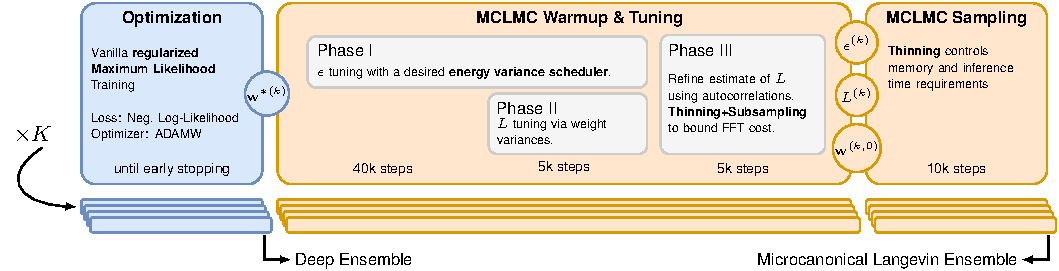
\includegraphics[width=\textwidth]{figures/project_summary/mile/mile_flowchart_ournotation.pdf}
\caption{The MILE procedure: optimization of $K$ ensemble members, MCLMC warmup and tuning (phases I--III,
step counts annotated), and sampling. The quantities carried between stages are circled: the optimized weights
$\mathbf w^{\ast(k)}$ of member $k$, and the step size $\epsilon^{(k)}$, decoherence length $L^{(k)}$ and initial
state $\mathbf w^{(k,0)}$ of its chain. Adapted from \citet[Fig.~1]{sommer2025mile} under CC BY 4.0, redrawn with
this report's notation ($\mathbf w$ for network weights, $\theta$ for the inferred parameters).}
\label{fig:mile}
\end{figure}

\subsection{Tempering and the prior scale}
\label{sec:bg_tempering}
With the posterior energy $U(\mathbf w)=-\sum_{i=1}^{n}\log p(y_i\mid x_i,\mathbf w)-\log p(\mathbf w)$, the Bayes
posterior is $p(\mathbf w\mid\mathcal{D})\propto\exp(-U(\mathbf w))$. \citet[App.~E]{wenzel2020cold} distinguish two
tempered versions at temperature $T>0$:
\begin{align}
\text{fully tempered:}\quad & p_{F}(\mathbf w\mid\mathcal{D})\propto\exp\!\big(-U(\mathbf w)/T\big)
  =p(\mathcal{D}\mid\mathbf w)^{1/T}\,p(\mathbf w)^{1/T},\\
\text{partially tempered:}\quad & p_{P}(\mathbf w\mid\mathcal{D})\propto p(\mathcal{D}\mid\mathbf w)^{1/T}\,p(\mathbf w)
  \notag\\
& \phantom{p_{P}(\mathbf w\mid\mathcal{D})}=\exp\!\Big(\log p(\mathbf w)+\tfrac1T\textstyle\sum_i\log p(y_i\mid x_i,\mathbf w)\Big).
  \label{eq:partial}
\end{align}
$T=1$ is the Bayes posterior and $T<1$ a ``cold'' posterior. A cold posterior sharpens the Bayes posterior,
``overcounting the data by a factor of $1/T$'' \citep[Sec.~2.2]{wenzel2020cold}; under full tempering the prior is
also rescaled to $p(\mathbf w)^{1/T}$. Their experiments use full tempering.
This project uses partial tempering, Eq.~\eqref{eq:partial}. Appendix~\ref{app:bg} relates it to the KL-weighted
evidence lower bound of variational BNNs, used by \citet{delaunoy2024lowbudget}, and shows that no prior reproduces it:
the prior that would turn a partially tempered posterior into a $T=1$ posterior depends on the training data.

\textbf{Per-observation form.} For the bivariate Gaussian head of Eq.~\eqref{eq:biv}, direct algebra gives
\begin{equation}
\label{eq:tempered_obs}
\mathcal{N}_2(\theta;\boldsymbol\mu,\Sigma)^{1/T}\;\propto\;\mathcal{N}_2(\theta;\boldsymbol\mu,T\Sigma)\cdot\det(\Sigma)^{-\frac12\left(\frac1T-1\right)},
\end{equation}
with a constant independent of the weights. At $T<1$ each training pair therefore enters the sampled posterior
through a Gaussian of covariance $T\Sigma$, narrower than the network's own, together with a factor that grows
as the predicted covariance shrinks. Tempering thus pulls the predicted mean towards the training targets and
the predicted width towards zero; the prior and the remaining residual term resist the second pull.
The temperature acts only in the MCLMC target, during warmup and sampling; pretraining and prediction are untempered,
so the test NLL of a tempered BNN is directly comparable with that of the other methods (Appendix~\ref{app:bg}).

\textbf{The cold posterior effect.} \citet{wenzel2020cold} find that predictive performance of deep BNNs is
best at $T<1$ (for a convolutional and long short-term memory network,
CNN-LSTM, on the IMDB movie-review sentiment task, roughly $0.01<T<0.2$), and state that they ``are not aware of any published
work demonstrating well-performing Bayesian deep learning at temperature $T=1$''. Proposed explanations include
data augmentation, under which \citet{izmailov2021bnn} find tempering ``not needed for near-optimal performance'',
and prior misspecification: heavy-tailed weight priors remove the effect in fully connected classifiers on
the MNIST and FashionMNIST image datasets, though not in convolutional or residual networks \citep{fortuin2022priors}.
\citet{noci2021disentangling} report that the effect ``becomes stronger for smaller dataset size $n$'', since ``the
relative influence of the prior over the likelihood increases with decreasing dataset size''. The task here has
no data augmentation and is studied precisely at small $n$, where these accounts predict the effect to be strongest
if the prior is the cause. Section~\ref{sec:variants} tests whether changing the prior can replace tempering.

\paragraph{Prior scale.}
\label{sec:bg_eb}
The scale of an isotropic prior $\mathcal N(\mathbf w;0,\tau^2I_d)$ can be set from the training data or without it.
Empirical Bayes (type-II maximum likelihood) maximizes the evidence $p(\mathcal D\mid\tau)$, whose stationary point is
MacKay's condition $\hat\tau^2=\lVert\mathbf m\rVert^2/\gamma$, with $\mathbf m$ the posterior mean and $\gamma\in[0,d]$
``the number of good parameter measurements'' \citep{mackay1992practical,mackay1992thesis}. MacKay himself uses separate
scales for hidden weights, hidden biases and output weights, since forcing one decay rate on all of them is
``inconsistent'' \citep{mackay1992thesis}. With a sampled posterior the expectations are Monte Carlo estimates:
stochastic-approximation updates with decreasing steps alternate with stochastic-gradient MCMC (SG-MCMC) in \citet{deng2019adaptive}, and the same
update, estimated from posterior samples, oscillates or diverges when applied per layer \citep{antoran2023sampling}. The
marginal likelihood also ``has a bias towards underfitting'' that weakens as data grow \citep{lotfi2022bayesian}, which
matters most at the smallest $n$. A data-free alternative chooses the $\tau$ whose prior predictive covers the
simulator's parameters with calibrated coverage, a single-scale version of the prior optimization of
\citet{delaunoy2024lowbudget}; it needs simulations outside the training budget, here 3{,}000: 1{,}000 pairs scored for coverage and 2{,}000 for
standardizing the inputs. A condition that needs
none follows from the law of total variance: any coherent posterior satisfies
$\mathbb E_x[\operatorname{Var}(\theta\mid x)]+\operatorname{Var}_x(\mathbb E[\theta\mid x])=\operatorname{Var}(\theta)$,
the second moment of the self-consistency that simulation-based calibration tests \citep{talts2018sbc}, and requiring
it of the untrained network on the $n$ training inputs fixes $\tau$ from the prior's moments alone. All three fit the
network's prior predictive to the simulator's joint distribution. For the first two, a well-specified model should
select the same scale (derivation and caveats in Appendix~\ref{app:bg}); on this task all three roughly agree,
within about 12\%, at $n=100$--$1{,}000$ (Section~\ref{sec:bnn_datafree}, Appendix~\ref{app:eb}). Agreement fixes the
scale within the isotropic Gaussian family, so the scale is well specified relative to MILE's default
$\mathcal N(0,1)$; it does not test whether an isotropic Gaussian is the right form of prior
(Section~\ref{sec:disc_adjust}).

\section{The RBF-kernel inference task}
\label{sec:data}

\subsection{Simulator}
\label{sec:simulator}
The parameter $\theta=(\sigma,\rho)$ is the amplitude and length scale of a squared-exponential (RBF)
kernel \citep{rasmussen2006gpml}, with independent truncated-normal priors
\begin{equation}
\sigma\sim\mathcal{N}(1.25,\,0.3^2)\big|_{\sigma>0},\qquad \rho\sim\mathcal{N}(0.60,\,0.2^2)\big|_{\rho>0}
\end{equation}
(the truncation removes $1.5\times10^{-5}$ and $1.3\times10^{-3}$ of the prior mass). One simulated
dataset is $N=10$ independent draws of a zero-mean process observed at $D=10$ equally spaced points
$t_1,\dots,t_D\in[0,1]$ with Gaussian noise $\eta=0.05$:
\begin{equation}
x_i\overset{\text{iid}}{\sim}\mathcal{N}(0,\,C_\theta),\qquad
(C_\theta)_{jk}=\sigma^2\exp\!\Big(-\frac{(t_j-t_k)^2}{2\rho^2}\Big)+\eta^2\delta_{jk},\qquad i=1,\dots,N .
\end{equation}
Every method sees only the empirical covariance $S=X^\top X/N$ ($X\in\mathbb{R}^{N\times D}$), flattened
to 100 numbers (55 distinct). Since the $x_i$ are zero-mean Gaussian, $S$ is sufficient for $\theta$, so
the summary loses no information. Figure~\ref{fig:simulator} shows draws and $S$ at three length scales.

\begin{figure}[h]
\centering
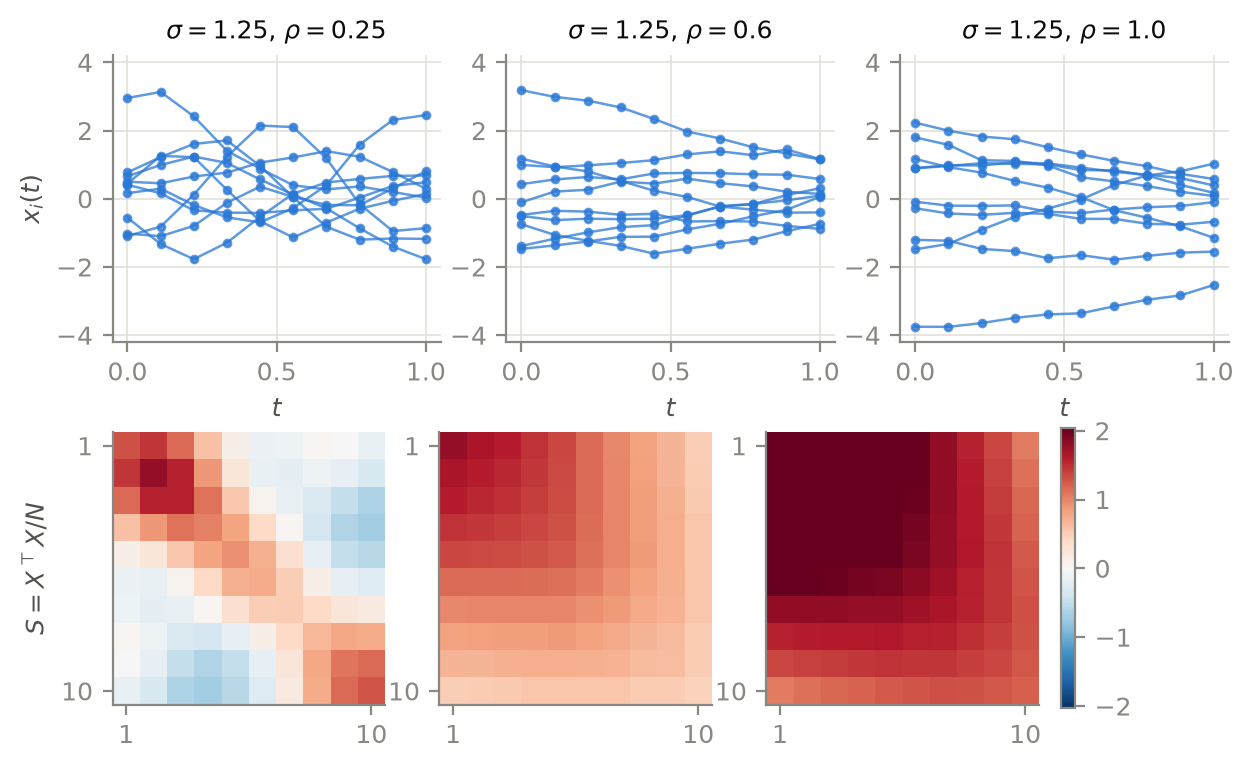
\includegraphics[width=0.85\textwidth]{figures/project_summary/rbf_task/simulator.png}
\caption{Top: the $N=10$ draws of one dataset at $\sigma=1.25$ and $\rho=0.25,\,0.60,\,1.00$. Bottom: the
summary $S$ each method receives. Draws re-simulated from the model for illustration.}
\label{fig:simulator}
\end{figure}

\subsection{Exact reference posterior}
\label{sec:reference}
With $S$ sufficient, the log-likelihood is
\begin{equation}
\log p(S\mid\theta)=-\frac{N}{2}\Big[\log\det C_\theta+\operatorname{tr}\!\big(C_\theta^{-1}S\big)\Big]+\text{const},
\end{equation}
and the posterior $p(\theta\mid S)\propto p(S\mid\theta)\,p(\theta)$ is evaluated on a $240\times240$ grid,
$\sigma\in[0.05,2.9]$, $\rho\in[0.02,1.6]$ (spacings 0.0119 and 0.0066), and normalized on the grid. Reference
moments are grid sums; $\log p(\theta^*\mid S)$ at the true parameter is bilinearly interpolated; reference
draws are sampled per cell with uniform jitter inside the cell.

On the 1{,}000 test datasets (Figures~\ref{fig:refpost}, \ref{fig:refsummary}) the posterior is
informative and correlated. Its standard deviation is 0.153 for $\sigma$ (RMS; 5--95\% range 0.121--0.169)
and 0.054 for $\rho$ (0.015--0.090), a median variance reduction relative to the prior of 73\% and 94\%. The
width grows with the parameter itself (correlation of posterior std with the true value 0.61 for $\sigma$,
0.91 for $\rho$). $\sigma$ and $\rho$ are positively correlated a posteriori in every test dataset (median
0.56, 5--95\% 0.44--0.65), so a predictive with independent marginals is misspecified here. The marginals
are mildly skewed (median skewness 0.42 for $\sigma$, 0.14 for $\rho$). As a check, the reference is
calibrated on the test set, as it must be when $\theta$ is drawn from the prior: the standardized error
$(\mathbb{E}[\theta\mid S]-\theta^*)/\mathrm{sd}[\theta\mid S]$ has standard deviation 1.02 / 0.97, and
69\% / 71\% of truths lie within one posterior standard deviation. It also satisfies the law-of-total-variance
condition of Section~\ref{sec:bg_eb}: the mean posterior variance plus the variance of the posterior mean is 0.0939
for $\sigma$ and 0.0379 for $\rho$, against test-set variances of $\theta^*$ of 0.0935 and 0.0376.

A per-dataset $300\times300$ refinement of the grid changes none of these summaries; only the two lowest-$\rho$ test
datasets change materially (Appendix~\ref{app:ref}).

\begin{figure}[h]
\centering
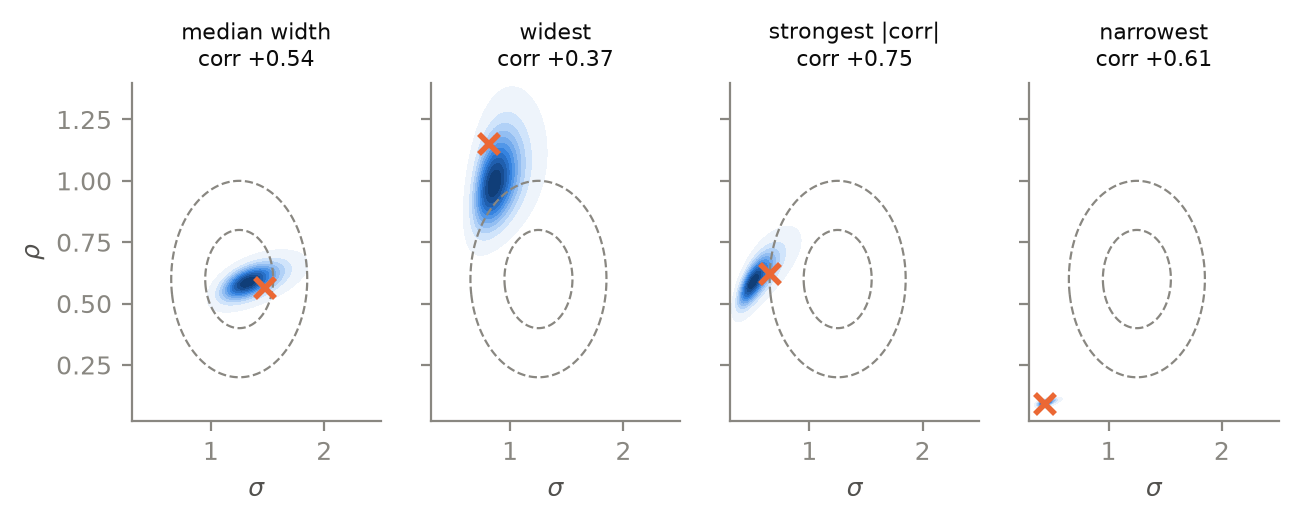
\includegraphics[width=\textwidth]{figures/project_summary/rbf_task/reference_posteriors.png}
\caption{Exact posterior (blue, normalized to its maximum) for four test datasets: median joint width, widest,
strongest correlation, narrowest. Dashed: prior at 1 and 2 standard deviations. Cross: true $\theta$.}
\label{fig:refpost}
\end{figure}
\begin{figure}[h]
\centering
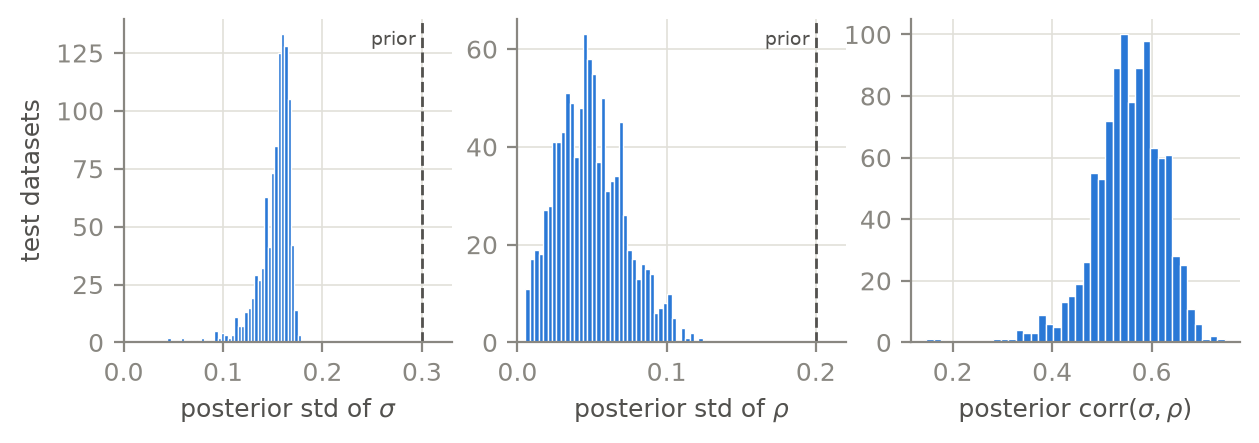
\includegraphics[width=\textwidth]{figures/project_summary/rbf_task/reference_summary.png}
\caption{Across the 1{,}000 test datasets: posterior standard deviation of $\sigma$ and $\rho$ (dashed: prior
standard deviation) and posterior correlation of $(\sigma,\rho)$.}
\label{fig:refsummary}
\end{figure}

\subsection{Datasets, training sizes and repeats}
\label{sec:datasets}
One canonical dataset is generated once (JAX key 0, split into 11{,}000 subkeys): a pool of 10{,}000 training
pairs $(S,\theta)$ and 1{,}000 test pairs. The test set is shared by every method, size and repeat. Training
sets of size $n\in\{50,100,500,1{,}000,5{,}000,10{,}000\}$ are nested subsamples of the pool: repeat $r$ takes the
first $n$ rows of one random permutation (NumPy generator seeded $123+r$), so the $n=50$ set is contained in the
$n=100$ set of the same repeat. All methods at a given $(n,r)$ train on identical rows, which makes every
comparison paired. Each fit's own seed is $100\,j+r$, with $j$ the index of $n$ in
$(10{,}000,\,5{,}000,\,1{,}000,\,500,\,100,\,50)$. Results use repeats $r=0,\dots,19$ at $n\le100$ and $r=0,\dots,4$
at larger $n$; the chain-wise diagnostics of Appendix~\ref{sec:res_rhat} use repeats 0--4 at every $n$. Because the pool has 10{,}000 rows,
repeats are nearly disjoint at small $n$ (two repeats share 1\% of their rows at $n=100$ and 10\% at $n=1{,}000$, on
average) but share half their rows at $n=5{,}000$ and all of them at $n=10{,}000$, where repeats differ only in seeds
and row order.

\subsection{Why this task}
\label{sec:why_task}

\paragraph{The exact posterior is known for every test dataset.}
Because $S$ is sufficient and $p(S\mid\theta)$ is Gaussian in closed form (Section~\ref{sec:reference}),
$p(\theta\mid S)$ itself is available on all 1{,}000 test datasets. The main comparison does not need it: methods are
scored mainly on the test NLL, which uses only the simulated $\theta^\ast$ (Section~\ref{sec:metrics}). The exact
posterior serves the appendices. Calibration tests that use only $\theta^\ast$ (TARP, SBC) are passed by the prior: a predictive
equal to $p(\theta)$ has exact coverage when $\theta^\ast$ is drawn from it. They detect a predictive that is too
narrow or too wide on average, but not how much wider than the posterior a calibrated predictive is. With the exact
posterior, each method's mean and width are compared with the posterior's, and the width warranted by the
method's own mean error is computable, and the BNN's split into aleatoric and epistemic uncertainty can be checked
(Appendices~\ref{app:width} and~\ref{app:moments}). Of the two questions of this report, whether a BNN beats NPE at
small $n$ is answered by the test NLL; whether the width it adds there is warranted needs the exact posterior.

\paragraph{The posterior width varies across datasets.}
Over the central 90\% of test datasets the posterior standard deviation ranges from 0.121 to 0.169 for $\sigma$ and
from 0.015 to 0.090 for $\rho$, and it grows with the parameter (correlation with the true value 0.61 and 0.91).
A predictive with one width for all inputs is wrong for most datasets, so each method must learn a
dataset-dependent width from $n$ examples. In the BNN this is the role of the aleatoric head, while the epistemic term should vanish
as $n$ grows; the exact target lets this split be checked (Appendix~\ref{app:width}).

\paragraph{The posterior has dependence and mild skew.}
$\sigma$ and $\rho$ are positively correlated a posteriori in every test dataset (median 0.56), so a predictive
with independent marginals is misspecified, and the marginal of $\sigma$ is right-skewed (median skewness 0.42;
0.14 for $\rho$). The BNN and the Gaussian predictor have a bivariate Gaussian head, which represents the dependence
but not the skew; NPE's flow can represent both. Both departures from an independent Gaussian are moderate, so no
method is badly misspecified, and differences that come from the predictive family are visible against the exact
moments rather than hidden by a gross misfit.

\paragraph{The summary is fixed and sufficient.}
Every method receives the same 100 numbers $S$, which lose no information about $\theta$
(Section~\ref{sec:simulator}). Differences between methods therefore come from the inference model and its
uncertainty, not from learning a summary of the $N=10$ replicated draws, which is a separate difficulty for neural
estimators \citep{sainsburydale2024neural}.

\paragraph{Simulation and evaluation are cheap.}
One simulation is ten draws from a 10-dimensional Gaussian, and one exact posterior is a $240\times240$ grid
evaluation. Training sets can therefore go down to $n=50$, every fit can be repeated on nearly independent training sets
at small $n$ (Section~\ref{sec:datasets}), and every comparison is paired on the same 1{,}000 test datasets. The prior is
informative but much wider than the posterior (median variance reduction 73\% for $\sigma$ and 94\% for $\rho$), so a
method that returns the prior is far from the target, and a method's width at small $n$ measures how much of the
information in $S$ it has learned.

\paragraph{Precedent.}
Inferring the amplitude and length scale of a squared-exponential covariance from Gaussian-process data is a
long-standing problem with a closed-form likelihood. \citet{williams1996gp} fit these hyperparameters by
optimization or average over them with hybrid Monte Carlo, \citet{neal1997mc} samples them with Markov chain
methods, and \citet{rasmussen2006gpml} give the standard treatment. \citet{murray2010slice} illustrate the posterior
over the length scale of a squared-exponential kernel given draws from the prior, the closest classical analogue of
this task. Bayesian inference of covariance parameters is equally established in spatial statistics, for the
Mat\'ern class \citep{handcock1993bayesian}. Approximate Bayesian computation uses tractable Gaussian processes
summarized by covariances as test problems: the
moving-average model of order 2, MA(2), with autocovariance summaries, compared with
exact-likelihood contours \citep{marin2012abc}, and an Ornstein--Uhlenbeck process scored against its true posterior
\citep{chen2021nass}. Recent amortized methods take the same targets: prior-fitted networks are checked against exact
Gaussian-process (GP) posterior predictives with an RBF kernel \citep{muller2022pfn}, the Amortized Conditioning
Engine (ACE) infers the length scale and output scale of a
one-dimensional GP \citep{chang2024ace}, \citet{bitzer2023amortized} amortize type-II maximum likelihood for kernels
built from squared-exponential components, and \citet{zammitmangion2024neural} compare amortized posterior methods,
including a normalizing-flow NPE, with MCMC on a Gaussian-process length scale over 1{,}000 test datasets. None of
the ten tasks of the standard SBI benchmark infers covariance parameters \citep{lueckmann2021benchmark}.

\paragraph{Relation to cosmological field inference.}
A stationary covariance function and its spectral density, or power spectrum, are Fourier duals (the
Wiener--Khintchine theorem), and the spectral density of the squared-exponential kernel in $d$ dimensions is
$\sigma^2(2\pi\rho^2)^{d/2}\exp(-2\pi^2\rho^2s^2)$ at frequency $s$ \citep[Sec.~4.2.1]{rasmussen2006gpml}. Each draw
$x_i$ is therefore a zero-mean Gaussian field whose parameters enter only through its power spectrum: $\sigma$ sets
the amplitude and $\rho$ the width in frequency, and the empirical covariance $S$ is the real-space counterpart of a
measured power spectrum. This is the simplest setting of cosmological parameter inference from fields.
\citet{makinen2021lossless} infer the amplitude $A$ and the scale dependence $B$ of a power spectrum $P(k)=Ak^{-B}$
from two-dimensional Gaussian random fields, which ``are relevant to early cosmological density fields such as the
Cosmic Microwave Background'', and compare simulation-based inference with the exact field-level posterior, as is
done here. The present task differs in the shape of the spectrum, Gaussian rather than a power law in frequency, and
in the data, ten noisy points of a one-dimensional field. The simulator extends without change to images and
three-dimensional volumes by placing the same kernel on a two- or three-dimensional grid; the likelihood stays
Gaussian, and on a periodic grid its covariance is diagonal in Fourier space \citep{makinen2021lossless}, so the
exact posterior remains available as a reference at larger scale. Beyond Gaussian fields, as for late-time galaxy
clustering, the power spectrum is no longer sufficient \citep{makinen2021lossless}, and a fixed sufficient summary
such as $S$ is no longer available.

\paragraph{Limitations.}
The tractable likelihood is what provides the exact reference and is the point of the task, not a limitation. The
main limitation is that all results come from this single task (Section~\ref{sec:disc_limits}). Its dimension is also
small: $\theta$ has two components and each dataset 55 distinct numbers, whereas analyses of
cosmological fields infer more parameters from far larger data, and how the comparison changes with the dimension
of $\theta$ and of the data is not tested. The summary is fixed and sufficient, so the methods are compared as
posterior estimators only; on fields, a summary or encoder must also be learned \citep{makinen2021lossless}, and how
that interacts with sampling the network's weights is not addressed. The posteriors have moderate dependence and
skew but are close to Gaussian. This does not favour the Gaussian heads of the BNN and the Gaussian predictor: NPE
with a bivariate Gaussian head in place of its flow is worse than with the flow (Appendix~\ref{app:npe_variants}).
Near-Gaussian posteriors are also the regime of well-constrained cosmological parameters, whose posteriors from Planck ``can be well
approximated as Gaussian for $\Lambda$CDM, as well as for many one- and two-parameter extensions''
\citep{huang2019correlations}; strongly non-Gaussian posteriors, which arise there for curvature, the dark-energy
equation of state or parameters bounded at zero \citep{huang2019correlations}, are not covered. The design is otherwise fixed: one kernel
family, fixed observation points and a fixed noise level. The training pool is 10{,}000 pairs, so repeats share
training rows at large $n$, and the spread over repeats there reflects seeds more than training sets.

\section{Methods}
\label{sec:methods}

\subsection{Common setup}
\label{sec:setup}
Each method maps the summary $S\in\mathbb{R}^{100}$ to a predictive density $q(\theta\mid S)$ over
$\theta=(\sigma,\rho)$, trained on $n$ pairs $(S_i,\theta_i)$ and evaluated on the shared 1{,}000 test datasets. Every
method is a 12-member ensemble, and at each $(n,r)$ all methods receive the same $n$ training rows
(Section~\ref{sec:datasets}). All training is full-batch. Within those rows, 20\% are held out for early stopping (10
of 50 at $n=50$), and every member of an ensemble uses its method's split. The BNN and the Gaussian predictor share
\code{bde}'s split (\code{train\_test\_split} with a fixed random state); NPE uses a permutation seeded with the fit's
seed. The two validation sets overlap only as much as independent random splits would (on average 1.9 of 10 rows at
$n=50$ and 4.3 of 20 at $n=100$), so the split adds noise to the paired comparisons but no systematic difference. The
held-out rows serve only for early stopping: the Gaussian predictor and NPE are fitted to 80\% of the training rows,
whereas the BNN's sampling stage conditions on all $n$ (Section~\ref{sec:bnn}), so the BNN uses 25\% more rows in its
final fit at every $n$. The BNN and the Gaussian predictor standardize inputs and targets by their mean and standard
deviation over the $n$ training rows, so that an $\mathcal{N}(0,1)$ weight prior is on the right scale, and map
predictions back; NPE sees raw $S$ and $\theta$.

\textbf{Gaussian heads.} The Gaussian predictor and the BNN output five numbers
$(\mu_\sigma,\mu_\rho,a_\sigma,a_\rho,c)$ per input, defining a bivariate normal
\begin{equation}
\label{eq:biv}
q(\theta\mid S)=\mathcal{N}_2\!\big(\theta;\,\boldsymbol\mu,\;\Sigma\big),\qquad
\Sigma=\begin{pmatrix}s_\sigma^2 & r\,s_\sigma s_\rho\\ r\,s_\sigma s_\rho & s_\rho^2\end{pmatrix},\qquad
s_\bullet=\mathrm{softplus}(a_\bullet)+10^{-6},\quad r=\tanh(c).
\end{equation}
Both are trained or sampled with this heteroskedastic likelihood; the correlation is fitted, since the exact posterior
is correlated in every test dataset (Section~\ref{sec:reference}).

\textbf{Uncertainty decomposition.} A BNN prediction is the equal-weight mixture of the Gaussians of its $C$
posterior draws ($C=12\times1{,}000$; Eq.~\ref{eq:mc_predictive}). Per parameter, by the law of total variance,
\begin{equation}
\label{eq:decomp}
\bar\mu=\tfrac1C\textstyle\sum_c\mu_c,\qquad
\underbrace{\tfrac1C\textstyle\sum_c s_c^2}_{\text{aleatoric}^2}
+\underbrace{\tfrac1C\textstyle\sum_c(\mu_c-\bar\mu)^2}_{\text{epistemic}^2}
=\text{total}^2 ,
\end{equation}
following \citet{kendall2017uncertainties}. The Gaussian predictor is the same mixture over its 12 networks ($C=12$),
so its epistemic term is the spread of the networks' means; a single network ($C=1$) has none. NPE has no such split.
The NPE ensemble is the equal-weight mixture of its 12 flows: its log density is the log-mean-exp of the flows', its
mean and standard deviation are the mixture's first two moments, and its calibration draws are taken in equal shares
from each flow.

\textbf{Predictive draws.} Calibration metrics use 1{,}000 draws per test dataset: from the Gaussian mixture for the
Gaussian predictor and the BNN, and from the flows for NPE (each flow's mean and standard deviation are taken from
5{,}000 of its draws). The log density at $\theta^*$ is exact for every method.

\subsection{Gaussian predictor}
\label{sec:gauss}
The Gaussian predictor is the BNN's network without sampling: the network of Section~\ref{sec:bnn}
($100\to16\to16\to16\to5$, soft-sign, the bivariate head of Eq.~\eqref{eq:biv}), with the BNN's member seeds, training
rows, early-stopping split, standardization, learning rate and weight decay. Each network is trained by AdamW
\citep{loshchilov2019adamw} on the negative log of Eq.~\eqref{eq:biv} to convergence. The validation NLL is evaluated
every 100 steps, training stops after 100 evaluations without an improvement of $10^{-4}$ (after at least 500 steps),
and the best parameters are kept. All 720 networks stopped early, none at the cap of 200{,}000 steps; the median last
step is 11{,}900 at $n=50$, rising to 33{,}400 at $n=10{,}000$ (maximum 67{,}500).

The BNN's chains start from the same networks pretrained under MILE's budget (at most 2{,}000 steps, patience 5
evaluations; Section~\ref{sec:impl}), and most of those stop at that cap: 148 of 240 networks at $n=50$, none at
$n=100$, 37 of 60 at $n=500$, all 60 at $n=1{,}000$, and 48 of 60 at $n=5{,}000$ and $10{,}000$. This capped version is
reported alongside the converged one. It isolates what sampling adds to the BNN's own starting point, while the
converged predictor measures it against networks whose optimization has finished. Both versions are evaluated as a
single network and as a 12-network ensemble.

\subsubsection{Single network}
\label{sec:gauss_single}
Member 0 of the 12, used alone ($C=1$ in Eq.~\eqref{eq:decomp}). Its predictive is one bivariate Gaussian, so its width
is aleatoric only, with no term for uncertainty about the network itself. It is compared with a single NPE flow at one
fitted network each; the two differ in head, encoder, optimizer and hyperparameters, not only in head.

\subsubsection{12-network ensemble}
\label{sec:gauss_ens}
The equal-weight mixture of the 12 networks ($C=12$), whose epistemic term is the spread of the networks' predicted
means (Eq.~\eqref{eq:decomp}); a deep ensemble in the sense of \citet{lakshminarayanan2017ensembles}. It has the same
ensemble size as the BNN and the NPE ensemble, so it is the comparison that separates the effect of sampling from the
effect of ensembling (Section~\ref{sec:intro}).

\subsection{Neural posterior estimator}
\label{sec:npe}
A conditional masked autoregressive flow \citep{papamakarios2017maf} in \code{nflows} \citep{durkan2020nflows},
trained as a neural posterior estimator \citep{papamakarios2016fast}. A context encoder
$g:\mathbb{R}^{100}\to\mathbb{R}^{8}$ (layers $100\to16\to16\to8$, ReLU) summarizes $S$. The flow maps a
standard normal on $\mathbb{R}^2$ through two blocks, each a masked affine autoregressive transform (a masked
autoencoder for distribution estimation, MADE, with 16 hidden units, one residual block, ReLU, conditioned on $g(S)$, scale $\mathrm{softplus}(\cdot)+\varepsilon$)
followed by reversing the variable order, so each parameter is transformed conditional on the other in one
of the two blocks. 3{,}920 parameters in total (encoder 2{,}024, flow 1{,}896). Training maximizes
$\sum_i\log q(\theta_i\mid S_i)$ with Adam \citep{kingma2015adam} and coupled ($L_2$) weight decay at a per-size
learning rate and weight decay (Section~\ref{sec:hp}), for up to 20{,}000 steps, evaluating the validation NLL every
100 steps and stopping after 20 evaluations without an improvement of $10^{-4}$; the best state is restored. Because
training $\theta_i$ are prior draws, maximizing this objective targets the posterior \citep{papamakarios2016fast}. The
flow gives exact $\log q(\theta^*\mid S)$ and draws; it has no aleatoric/epistemic split. Like the Gaussian predictor,
NPE is evaluated as a single flow and as a 12-flow ensemble. Two one-change variants, an encoder of the BNN's width
($100\to16\to16\to16$) and a bivariate Gaussian head in place of the flow, are in Appendix~\ref{app:npe_variants}.

\subsubsection{Single flow}
\label{sec:npe_single}
One flow trained as above, with the fit's seed. It is member 0 of the ensemble below.

\subsubsection{12-flow ensemble}
\label{sec:npe_ens}
Twelve flows on the same training rows and early-stopping split, differing only in their initialization seeds
($s+10{,}000\,k$ for member $k$, with $s$ the fit's seed, so member 0 is the single flow). The ensemble is the
equal-weight mixture of the 12 flows (Section~\ref{sec:setup}), the deep-ensemble construction that
\citet{hermans2022trust} find ``provides more reliable approximations'' and that \citet{delaunoy2024lowbudget} use, with
5 members, as a baseline. It has the same ensemble size as the BNN and the Gaussian predictor ensemble.

\textbf{Long-trained ensemble at $n=10{,}000$.} At the default budget the flows at $n=10{,}000$ are under-trained: the
one member whose stopping step was checked (repeat 0, member 0) ran to the 20{,}000-step cap with its best state at
step 19{,}700 (the default-budget runs did not record stopping steps otherwise). A second ensemble at $n=10{,}000$,
repeats 0--4, is identical except for a cap of 200{,}000 steps and a patience of 100 evaluations. Every flow stopped
early, with its best state at a median step of 30{,}000--51{,}000 depending on the repeat (at most 84{,}400 steps
run). This long-trained ensemble is the NPE comparator at $n=10{,}000$ wherever stated.

\subsection{Bayesian neural network}
\label{sec:bnn}
\textbf{Network.} A fully connected network $f_{\mathbf w}:\mathbb{R}^{100}\to\mathbb{R}^5$ with three hidden
layers of width 16, the soft-sign activation $x/(1+|x|)$ on every hidden layer, and a linear output layer:
$100\to16\to16\to16\to5$, $d=2{,}245$ weights and biases. Soft-sign is used because \code{bde} offers no
$\tanh$; it is smooth and saturating like $\tanh$, with heavier tails. The five outputs parameterize the
bivariate normal of Eq.~\eqref{eq:biv} in standardized units.

\textbf{Likelihood, prior, posterior.} With $\tilde S_i,\tilde\theta_i$ the standardized training pairs,
\begin{equation}
p(\mathcal{D}\mid\mathbf w)=\prod_{i=1}^{n}\mathcal{N}_2\!\big(\tilde\theta_i;\,\boldsymbol\mu_{\mathbf w}(\tilde S_i),\,
\Sigma_{\mathbf w}(\tilde S_i)\big),\qquad
p(\mathbf w)=\prod_{j=1}^{d}\mathcal{N}(w_j;0,1),\qquad
p(\mathbf w\mid\mathcal{D})\propto p(\mathcal{D}\mid\mathbf w)\,p(\mathbf w).
\end{equation}
The $\mathcal{N}(0,1)$ prior on every weight and bias is MILE's default \citep{sommer2025mile}. The variants below
make one change each, everything else fixed: a prior scale chosen without training data, a tempered likelihood, and a
scale chosen by empirical Bayes.

\textbf{Prediction.} The posterior is sampled with MILE (Section~\ref{sec:mile}): $K$ members, $S=1{,}000$ kept
draws each. The predictive for a test summary $S^\ast$ is the equal-weight mixture over all $KS$ draws
(Eq.~\ref{eq:mc_predictive}), mapped back to original units by $\boldsymbol\mu\mapsto\boldsymbol\mu\odot\mathbf{s}_y+\mathbf{m}_y$
and $s_\bullet\mapsto s_\bullet\,s_{y,\bullet}$ (training-set target mean $\mathbf m_y$ and standard deviation
$\mathbf s_y$); the correlation $r$ is unchanged, being invariant under a positive per-coordinate rescaling. Its
first two moments split into aleatoric and epistemic parts as in Eq.~\eqref{eq:decomp}. Mixing is assessed on
these predictive quantities, never on raw weights, whose permutation and scaling symmetries make weight-space
diagnostics uninterpretable \citep{izmailov2021bnn,sommer2024connecting}.

\subsubsection{Data-free prior scale}
\label{sec:bnn_datafree}
The prior is $\mathcal{N}(0,\tau^2)$ on every weight and bias with $\tau=0.3655$, chosen before any training data are
seen. The prior predictive of the untrained network, with weights and biases drawn from $\mathcal{N}(0,\tau^2)$, is
scored by TARP coverage \citep{lemos2023tarp} on 1{,}000 simulated pairs $(\theta,x)$ drawn independently of the
canonical dataset (the same pairs in every trial), with 1{,}000 weight draws; inputs are standardized by the mean and standard deviation of 2{,}000
further simulated $x$, and outputs are mapped to $\theta$ with the prior mean and standard deviation. With
$\mathrm{ECP}(\alpha)$ the expected coverage probability, the fraction of datasets whose true parameter lies inside
TARP's credible region at credibility level $\alpha$, which equals $\alpha$ for a calibrated estimator
(Appendix~\ref{app:moments}), $\tau$ minimizes the absolute area between the coverage curve and the diagonal, $\big|\int(\mathrm{ECP}(\alpha)-\alpha)\,\mathrm{d}\alpha\big|$,
by Bayesian optimization (\code{scikit-optimize}, Gaussian-process surrogate, expected improvement, 40 trials,
$\tau$ log-uniform on $[10^{-3},3]$). This is a single-scale version of the prior optimization of
\citet{delaunoy2024lowbudget}; it uses 3{,}000 simulations outside the training budget but no training pairs.

\textbf{Simulation-free check.} The same scale follows from the coherence condition of Section~\ref{sec:bg_eb} without
extra simulations. For each candidate $\tau$ (81 values, log-spaced on $[0.05,2]$), the untrained network's predictive
over 2{,}000 weight draws, standardized as in training, is evaluated on the $n$ training inputs, and the ratio
$\big(\overline{s_j^2}+\widehat{\operatorname{Var}}(\mu_j)\big)/V_j^\ast$ is computed for each parameter $j$, with the
averages taken over weight draws and inputs and $V_j^\ast$ the truncated-normal prior variance in standardized units.
Each ratio crosses 1 exactly once; the selected scale minimizes the sum of the squared log ratios. It is
$\tau=0.377\pm0.053$ at $n=50$, $0.364\pm0.024$ at $n=100$, $0.353\pm0.008$ at $n=500$ and $0.347$ at $n=1{,}000$
(mean $\pm$ sd over repeats), so the simulator-calibrated $0.3655$ lies within the repeat spread at $n=50$ and within
5\% at larger $n$. The spread at $n=50$ comes from standardizing the targets by the standard deviation of 50 draws: over
repeats and parameters, the selected scale correlates at $-0.998$ with that standard deviation divided by the prior's.
Under $\mathcal{N}(0,1)$ the untrained predictive implies about ten times the prior variance. The check sets the scale
of no run.

\subsubsection{Tempered likelihood}
\label{sec:bnn_temp}
The likelihood is partially tempered (Eq.~\eqref{eq:partial}): in warmup and sampling the MCLMC target is
$\log p(\mathbf w)+\tfrac1T\log p(\mathcal{D}\mid\mathbf w)$, with the $\mathcal{N}(0,1)$ prior unscaled; pretraining
and prediction are untempered. $T$ is chosen per size on the grid $0.2,0.3,\dots,1.0$, by bisection on the sign of the
local slope and always including $T=1$, minimizing the mean validation NLL of 3-member fits over the training sets of repeats 0--2 (Appendix~\ref{app:temp_search}). The
validation data are the 1{,}000 pool rows that follow the training rows in each repeat's permutation, and the reported
$T$ is the argmin over every evaluated point. The search uses the runs' own learning rate and weight decay. It gives
$T=0.7$, $0.7$, $0.6$ and $0.7$ at $n=50$, $100$, $500$ and $1{,}000$. At $n\ge5{,}000$ the best temperature is close to 1, so the $\mathcal N(0,1)$ BNN is there
both the untempered and, approximately, the optimally tempered BNN, and no separate tempered model is run. The grid
search was not run at these sizes; the evidence is that the selected temperature rises with $n$ (0.6--0.7 at
$n=500$--$1{,}000$), as does the coldest temperature at which the chains still mix (Appendix~\ref{app:temp_search}), and
that the only tempered runs at $n=5{,}000$ and $10{,}000$, earlier 3-member fits at $T=0.305$ transferred from an
$n=100$ search, are worse than $T=1$ under the same settings (test NLL $-1.88$ against $-2.21$ and $-2.25$ against
$-2.27$) and do not mix (maximum $\widehat R$ 32--64).

\subsubsection{Empirical Bayes}
\label{sec:bnn_eb}
One scale $\tau$ for all 2{,}245 weights and biases is updated during sampling, on the re-tuning sampler of
Appendix~\ref{sec:retune}: the 10{,}000 sampling steps are split into 10 segments of 1{,}000, and $(\epsilon,L)$ are
re-tuned (200 and 50 steps) after each, so a chain runs 12{,}500 steps. $\tau$ starts at the root-mean-square of the
member's pretrained weights, under which the warmup runs. After each segment, with $m_i$ and $v_i$ the mean and
variance of weight $i$ over that segment's steps,
\begin{equation}
\label{eq:eb_block}
\gamma=d-\sum_i v_i/\tau^2\ \ (\text{clamped to }[1,d]),\qquad \tau_{\mathrm{target}}^2=\sum_i m_i^2/\gamma,
\end{equation}
MacKay's condition (Section~\ref{sec:bg_eb}) with the posterior mean and covariance replaced by the segment's sample
moments. $\log\tau$ then moves halfway towards $\log\tau_{\mathrm{target}}$, by at most a factor of 2 per update, with a
floor of $10^{-3}$. The scale is per member, and all 1{,}000 kept draws per chain are used, including those drawn before
the scale has settled. The damping, the step cap and the floor have no source. The fixed-scale control,
$\mathcal{N}(0,1)$ + retune, is the same sampler with $\tau=1$.

\subsection{Our MILE implementation}
\label{sec:impl}
We use the \code{sklearn-contrib-bde} package (version 1.0.2, \code{blackjax} 1.2.2), which implements MILE.
Its settings match the paper's defaults: $K=12$ members per fit, 50{,}000 warmup steps split $0.8/0.1/0.1$ into phases
I--III ($40{,}000/5{,}000/5{,}000$), 10{,}000 sampling steps thinned by 10 to 1{,}000 draws per chain, EEVPD target
annealed $0.5\to0.1$, ESS target 100, initial step size equal to the pretraining learning rate, no preconditioning, and
an isotropic $\mathcal{N}(0,1)$ prior on all 2{,}245 weights. Each member is pretrained by AdamW on the negative log of
Eq.~\eqref{eq:biv} for at most 2{,}000 steps, evaluating the validation NLL every 100 steps and stopping after 5
evaluations without an improvement of $10^{-4}$ (after at least 500 steps), on \code{bde}'s 80/20 split
(Section~\ref{sec:setup}); the best parameters are kept, and chain $k$ starts from member $k$. The network and
likelihood are those of Section~\ref{sec:bnn}. The per-draw outputs give the chain-wise diagnostics of
Appendix~\ref{sec:res_rhat}.

Departures from stock \code{bde} are subclass overrides in \code{src/rbf\_sbi/bnn.py} (Appendix~\ref{app:bde}): a correlated
two-target head; a pretraining schedule that evaluates every 100 steps, with AdamW; replacement of members whose chains
become non-finite; likelihood tempering in warmup and sampling; and, for the empirical-Bayes model and its control,
periodic re-tuning of $(\epsilon,L)$ during sampling and the block update of the prior scale
(Section~\ref{sec:bnn_eb}).

\subsection{Hyperparameter selection}
\label{sec:hp}
Only the learning rate and weight decay are searched, per method and training size; MILE's sampler settings are its
defaults. NPE's are chosen by Bayesian optimization \citep{snoek2012practical}: \code{scikit-optimize} 0.10.2, a Gaussian-process surrogate with expected
improvement, log-uniform search ranges $\mathrm{lr}\in[10^{-5},10^{-1}]$ and $\mathrm{wd}\in[10^{-7},10^{-2}]$,
10 random initial points, random state 123, and a wall-clock budget per size. The objective is the validation NLL on an 80/20
split of the repeat-0 training rows. Within its budget the search ran 3--20 trials per size and acted as a random search
of 3--10 points (Appendix~\ref{app:hp}). The BNN and the Gaussian predictor are not tuned by Bayesian optimization: they
share one pair per size,
chosen on a grid for the BNN's network as a standalone predictor: one network pretrained exactly as in
Section~\ref{sec:impl}, without sampling, scored by its NLL on 1{,}000 held-out pool rows averaged over the training
sets of repeats 0--2. The grid has 17 learning rates from $10^{-5}$ to $10^{-1}$ in quarter decades and 15 weight decays
from $10^{-7}$ to $1$ in half decades (the upper bound is raised from $10^{-2}$ because AdamW's decoupled decay is
nearly inert below it at these learning rates), and the argmin is used at every size. At $n=50$ the argmin is
noise-driven, and at its learning rate two of the three grid fits stop at the 2{,}000-step cap. The converged Gaussian
predictor keeps these values, which were chosen under the 2{,}000-step budget. Search details, budgets and rationale, including the earlier BNN
search on the full MILE fit that this grid supersedes: Appendix~\ref{app:hp}.

\begin{table}[h]
\centering\small
\begin{tabular}{rcccc}
\toprule
 & \multicolumn{2}{c}{NPE} & \multicolumn{2}{c}{BNN and Gaussian predictor} \\
\cmidrule(lr){2-3}\cmidrule(lr){4-5}
$n$ & lr & wd & lr & wd \\
\midrule
50      & $9.53\times10^{-5}$ & $2.98\times10^{-4}$ & $3.16\times10^{-5}$ & $3.16\times10^{-1}$ \\
100     & $3.23\times10^{-3}$ & $4.18\times10^{-6}$ & $1.78\times10^{-4}$ & $3.16\times10^{-1}$ \\
500     & $2.37\times10^{-3}$ & $1.44\times10^{-4}$ & $1.78\times10^{-4}$ & $1.00\times10^{-2}$ \\
1{,}000 & $5.80\times10^{-3}$ & $3.94\times10^{-4}$ & $1.78\times10^{-4}$ & $3.16\times10^{-1}$ \\
5{,}000 & $4.40\times10^{-4}$ & $7.92\times10^{-5}$ & $1.00\times10^{-3}$ & $3.16\times10^{-1}$ \\
10{,}000& $9.21\times10^{-4}$ & $7.95\times10^{-4}$ & $1.00\times10^{-3}$ & $3.16\times10^{-1}$ \\
\bottomrule
\end{tabular}
\caption{Learning rate and weight decay used by every result in this document. The BNN values apply to all BNN
variants and to the Gaussian predictor (capped and converged).}
\label{tab:hp}
\end{table}

\subsection{Software, compute and use of language models}
\label{sec:compute}
All fits ran on the Perlmutter system of the National Energy Research Scientific Computing Center (NERSC), one
NVIDIA A100 GPU (40 or 80\,GB) per Slurm job. For one training set, a 12-chain BNN under stock MILE takes 36--72\,s of
wall time (fitting and prediction; the 12 chains run in parallel on the GPU), the re-tuning sampler 411--534\,s, the
converged 12-network Gaussian predictor 24--82\,s, and the 12-flow NPE ensemble 157--238\,s at $n\le1{,}000$ and
663--907\,s at $n\ge5{,}000$; Appendix~\ref{app:hp} gives the settings per model and Appendix~\ref{app:repro} the
software versions; the code is at \url{https://github.com/sam-dowd/rbf-sbi-bnn}. The code, analysis scripts and text of this report were developed with the assistance of Claude
models (Anthropic), most recently Claude Opus 5.5, used through Claude Code; all results were checked by the author.

\section{Evaluation protocol}
\label{sec:eval}

\subsection{Metrics}
\label{sec:metrics}
All metrics are computed on the $M=1{,}000$ test datasets $(S_j,\theta^\ast_j)$.

\textbf{Test NLL.} The primary score is
\begin{equation}
\label{eq:nll}
\mathrm{NLL}=-\frac1M\sum_{j=1}^{M}\log q(\theta^\ast_j\mid S_j)\quad\text{(nats, joint over }(\sigma,\rho)\text{)},
\end{equation}
in nats (natural-log units). It needs only the true parameter $\theta^\ast_j$, not the exact posterior. It rewards
accuracy and penalizes miscalibration in either direction, but over-confidence much more than conservatism: a width
that is too narrow enters through the squared standardized error, one that is too wide only through its logarithm.
That asymmetry suits scientific use, where a conservative posterior is the safer error (Section~\ref{sec:intro}). Each method's $q$ is a normalized
density on $\theta$ in original units, evaluated exactly at $\theta^\ast_j$: the mixture of the 12 networks' Gaussians
for the Gaussian predictor (one Gaussian for a single network), the equal-weight mixture over all $KS$ draws for the
BNN, the flow's change-of-variables density for a single flow and the mixture of the 12 flows' densities for the NPE
ensemble, and the grid density for the exact posterior (Appendix~\ref{app:ref}), so all NLLs are directly comparable.
The test NLL is the negative of the mean log pointwise predictive density (LPPD) at $\theta^\ast$, the predictive score
of \citet{sommer2024connecting}. The exact posterior scores $-2.390$.

\textbf{Badly over-confident datasets.} With $\hat\mu_{j,p}$ and $\hat s_{j,p}$ the mean and total standard deviation of a
method's predictive for parameter $p$ (Section~\ref{sec:setup}), $z_{j,p}=(\hat\mu_{j,p}-\theta^\ast_{j,p})/\hat s_{j,p}$. The
percentage of test datasets with $|z_{j,p}|>3$ for $\sigma$ or $\rho$ counts the datasets on which the predictive is far
too narrow for its own error. The exact posterior scores 0.9\%, somewhat more than the 0.5\% of a Gaussian, since its
posteriors are not exactly Gaussian.

\textbf{Metrics that use the exact posterior.} Four appear in Section~\ref{sec:experiments}; each is defined in full
where it is reported. The \emph{TARP coverage area} is the integral over credibility levels $\alpha$ of
$\mathrm{ECP}(\alpha)-\alpha$: 0 for a calibrated predictive, positive for a conservative one, negative for an
over-confident one (Appendix~\ref{app:moments}). The \emph{width over warranted width} is the RMS predictive width
divided by the RMS width that a calibrated predictive with the same mean errors would need; 1 is ideal
(Appendix~\ref{app:width}). The \emph{coherence ratio} is the mean predicted variance plus the variance of the predicted
means across test datasets, divided by the variance of $\theta^\ast$ over the test set; by the law of total variance
(Section~\ref{sec:bg_eb}) it is 1 for a coherent predictive (Appendix~\ref{app:width}). The \emph{aleatoric share} is
the fraction of a BNN's variance in excess of the exact posterior's and of its own mean error that lies in its
aleatoric term (Eq.~\eqref{eq:decomp}). The appendices add the error of the predicted mean and of the predicted
standard deviation against the exact posterior's and the spread of $z$ (Appendix~\ref{app:moments}); and the decomposition of the BNN's NLL into chains, draws and
starting networks (Appendix~\ref{app:inside}). Table~\ref{tab:exactfloor} gives their values for the exact posterior.

\subsection{Convergence diagnostics}
\label{sec:convdiag}
Diagnostics are reported, never used to accept or discard a fit. The only members removed are those whose draws
become non-finite. Under stock MILE (the $\nzo$, data-free and tempered BNNs) they are replaced by re-seeded refits on
the same training rows, so every fit has 12 members (8 of 2{,}136 member fits failed). The re-tuning sampler (the
$\nzo$ + re-tune and empirical-Bayes models, Appendix~\ref{app:eb}) drops them without replacement, which leaves 9--11
members in 19 of 60 and 8 of 60 fits respectively.
BNN weight posteriors are non-identifiable and multimodal, chains started in different modes need not reach a common
function \citep[Sec.~6.2]{sommer2024connecting}, and MILE claims no convergence \citep[App.~A.3]{sommer2025mile}; fits are judged
by their test NLL (Section~\ref{sec:metrics}) and, in the appendices, by their agreement with the exact posterior. The pipeline diagnostic is the classic potential scale reduction
factor (PSRF) $\widehat R$ \citep{gelman1992inference} with the effective sample size, as implemented in BlackJAX 1.2.2, on the
predicted mean for every (test dataset, parameter) pair with the $K$ members as chains, reported as maximum and mean.
Appendix~\ref{app:diag} adds rank-normalized $\widehat R$, both pooled (all members' chains together, so it measures
whether the members agree) and chain-wise (each chain split into sub-chains, so it measures whether each chain is
stationary), on the mean, the width and the log density
at $\theta^\ast$, and the per-member expanding-window LPPD: the test LPPD of a member's predictive built from its first
$l$ kept draws, as a function of $l$, the per-chain convergence check of \citet[App.~B.2]{sommer2024connecting}.

\subsection{Paired comparisons}
\label{sec:paired}
All methods at a given $(n,r)$ train on the same rows and are evaluated on the same test set
(Section~\ref{sec:datasets}). A comparison between two methods $A$ and $B$ is therefore made per repeat,
$\Delta_r=m_A(n,r)-m_B(n,r)$ for a metric $m$, which removes the variation due to which training set was drawn
(at low $n$ the largest source of variation). Differences are reported as
\[
\bar\Delta\pm\mathrm{sd}(\Delta)\ \ (k/R),
\]
the mean and sample standard deviation of $\Delta_r$ over the $R$ repeats ($R=20$ at $n\le100$, $R=5$ above) and the
number $k$ of repeats in which the difference has the stated sign; for NLL, negative means $A$ is better. A difference
is called a finding if a two-sided paired $t$-test on the $\Delta_r$ gives $p<0.05$. A Wilcoxon signed-rank test, which
does not assume normality, is reported as a check, and cells in which the two disagree are marked. A statement about a
single fit requires a difference larger than the chain-to-chain spread within that fit. The spread of a metric over
repeats is itself reported, as a method's consistency across training sets. At $n\le1{,}000$ repeats share at most
10\% of their training rows; at $n=5{,}000$ and $10{,}000$ they share half or all of them (Section~\ref{sec:datasets}),
so the spread there is mostly seed variance. 

GPU runs are not bit-reproducible: identical code, seed and data give different chains (e.g.\ empirical-Bayes
prior scales differing by 0.01--0.02). ``Reproduces'' therefore means agreement within the spread above. For
example, re-running the 3-member $\nzo$ configuration used before the final runs at $n=100$, $r=0$ gave test NLL
$-0.759$ against the saved $-0.745$, inside that configuration's repeat-to-repeat spread of 0.108, with the pooled
predicted mean within the saved run's between-chain spread.

\section{Experiments}
\label{sec:experiments}
This section reports test NLL, the primary score (Section~\ref{sec:metrics}), and in
Section~\ref{sec:variants} also the width metrics that use the exact posterior. Three BNNs are compared, each a
12-chain MILE fit, under MILE's default $\mathcal N(0,1)$ prior, with the data-free prior scale
(Section~\ref{sec:bnn_datafree}) and with a tempered likelihood (Section~\ref{sec:bnn_temp}); ``the BNN'' means any of
the three. The tempered BNN is run only at $n\le1{,}000$, since at larger $n$ the best temperature is close to 1 and the
$\mathcal N(0,1)$ BNN is also the tempered one. Section~\ref{sec:res_single} compares the BNNs with a single network of
each baseline, so that they differ from it in both sampling and ensembling, and Section~\ref{sec:res_ens} compares them
with 12-member ensembles of the same baselines, so that only sampling differs. Paired differences, the verdict of each BNN against
each ensemble, the decomposition of the BNN's NLL, calibration and width are in Appendix~\ref{app:final}.

\subsection{Sampling and ensembling together: the BNN against single networks}
\label{sec:res_single}
\label{sec:baseline}
\begin{table}[h]
\centering
\small\setlength{\tabcolsep}{3.5pt}
\resizebox{\textwidth}{!}{%
\begin{tabular}{lcccccc}
\toprule
 & $n=50$ & $n=100$ & $n=500$ & $n=1{,}000$ & $n=5{,}000$ & $n=10{,}000$ \\
\midrule
\inputrows{tables/section6_single_nll.tex}
\bottomrule
\end{tabular}}
\caption{Test NLL (nats), mean $\pm$ sd over repeats: 20 repeats at $n\le100$, 5 at $n\ge500$; lower is better; exact posterior $-2.390$. Bold, per column: the lowest mean and every row not distinguishable from it by a two-sided paired $t$-test at $p<0.05$ (Section~\ref{sec:paired}). $^\dagger$: at $n\le100$ the Wilcoxon signed-rank test disagrees with the bolding. The one dagger: the single network at $n=50$ is bolded only because one repeat at
$+32.1$ inflates its sd (median over repeats $-0.34$). Gaussian predictor: one converged network (member 0); NPE: one
flow (member 0 of the ensemble).}
\label{tab:sec6_single}
\end{table}

\begin{figure}[h]
\centering
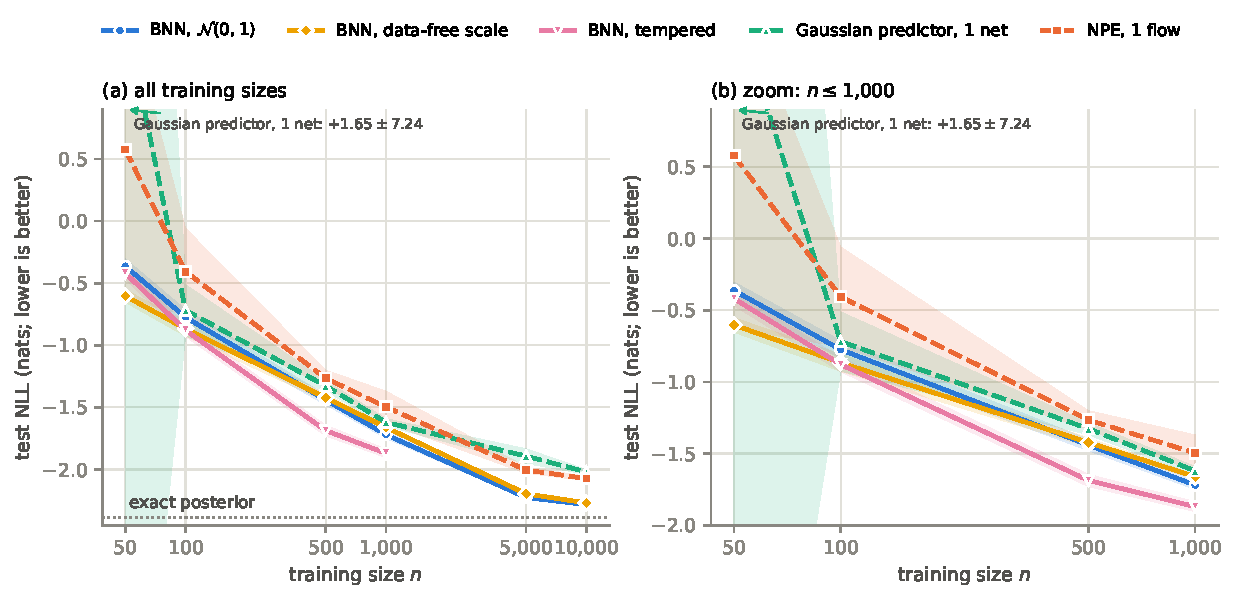
\includegraphics[width=\textwidth]{figures/project_summary/section6/nll_single.pdf}
\caption{Test NLL against $n$ for the three BNNs and the single networks of Table~\ref{tab:sec6_single}: mean over
repeats, band $\pm1$ sd over repeats. Means above the plotted range are written at the top edge.}
\label{fig:sec6_single}
\end{figure}

Against a single network, sampling looks decisive (Table~\ref{tab:sec6_single}, Figure~\ref{fig:sec6_single}). Every
BNN is below a single NPE flow at every $n$, by about 1 nat at $n=50$ and 0.4 at $n=100$, and below a single
Gaussian-predictor network from $n=500$, the data-free and tempered BNNs also at $n=100$. At $n=50$ the paired test
separates no BNN from the single Gaussian-predictor network, because one of its 20 repeats scores $+32$, although the
BNNs are lower on most repeats. The larger difference at small $n$ is reliability: over training sets, a single
network's NLL has a standard deviation of 0.2--7 nats at $n\le100$, every BNN's 0.05--0.06. A single network fitted to
50 or 100 simulations is a poor and unpredictable estimator. How much of the BNN's advantage over it comes from sampling,
and how much from averaging over many networks, is what the comparison with ensembles separates.

\subsection{Sampling alone: the BNN against 12-member ensembles}
\label{sec:res_ens}
\begin{table}[h]
\centering
\small\setlength{\tabcolsep}{3.5pt}
\resizebox{\textwidth}{!}{%
\begin{tabular}{lcccccc}
\toprule
 & $n=50$ & $n=100$ & $n=500$ & $n=1{,}000$ & $n=5{,}000$ & $n=10{,}000$ \\
\midrule
\inputrows{tables/section6_ensemble_nll.tex}
\bottomrule
\end{tabular}}
\caption{Test NLL (nats), mean $\pm$ sd over repeats: 20 repeats at $n\le100$, 5 at $n\ge500$; lower is better; exact posterior $-2.390$. Bold, per column: the lowest mean and every row not distinguishable from it by a two-sided paired $t$-test at $p<0.05$ (Section~\ref{sec:paired}). $^\dagger$: at $n\le100$ the Wilcoxon signed-rank test disagrees with the bolding. Gaussian predictor: the 12 networks trained to convergence; NPE: 12 flows at the default
budget, and at $n=10{,}000$ also the long-trained ensemble (Section~\ref{sec:npe_ens}). Lower block: percentage of the
1{,}000 test datasets on which the predictive is badly over-confident, $|z|>3$ for $\sigma$ or $\rho$ with
$z=(\text{predicted mean}-\theta^\ast)/\text{predicted sd}$; median over repeats, worst repeat in parentheses; the exact
posterior scores 0.9\%.}
\label{tab:sec6_ens}
\end{table}

\begin{figure}[h]
\centering
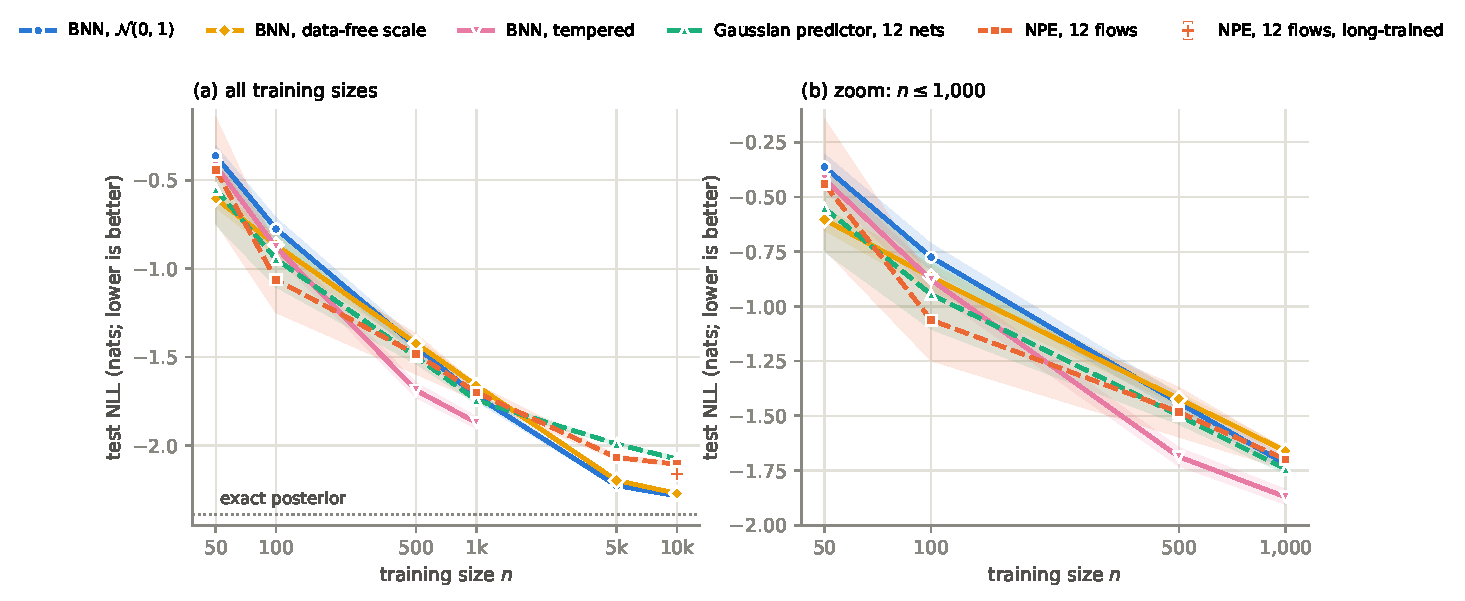
\includegraphics[width=\textwidth]{figures/project_summary/section6/nll_ensemble.pdf}
\caption{Test NLL against $n$ for the three BNNs and the 12-member ensembles of Table~\ref{tab:sec6_ens}: mean over
repeats, band $\pm1$ sd over repeats; the long-trained NPE at $n=10{,}000$ as a single marker with its sd.}
\label{fig:sec6_ens}
\end{figure}

Against these equally ensembled baselines the BNN does not have the lowest average NLL at $n\le100$, but it is the
most reliable estimator there, and it has the lowest NLL from $n=500$ with a tempered likelihood and from $n=5{,}000$
without. Ensembling removes most of the single-network advantage. Twelve flows lower NPE's NLL by about 1 nat at $n=50$ and 0.7 at $n=100$,
and twelve networks lower the Gaussian predictor's by 0.23 at $n=100$, so against equally ensembled baselines the BNN
no longer wins at small $n$ (Table~\ref{tab:sec6_ens}, Figure~\ref{fig:sec6_ens}).

\textbf{Small $n$: NPE is as good or better on average.} At $n=100$ the 12-flow NPE has the lowest NLL of all models,
0.18--0.29 nats below every BNN. At $n=50$ the comparison is close: only the data-free BNN is below NPE, by
$0.16\pm0.28$ nats on 13 of 20 repeats. All repeats share one test set, whose sampling uncertainty the paired test does
not include; for this comparison it is about 0.05 nats, comparable to the repeat-to-repeat standard error of 0.06, so the
difference is marginal, and it comes from the prior rather than from sampling, since this BNN ties its own unsampled
networks. Neither adjustment rescues $n=100$. NPE's advantage there is in the predicted mean: the 12-flow ensemble's
mean error is 0.10 for $\sigma$ and 0.09 for $\rho$, against 0.12--0.13 and 0.10--0.11 for the BNNs
(Appendix~\ref{app:moments}), and neither adjustment changes the BNN's mean error at $n\le100$ by more than 0.006. The
advantage in $\sigma$, whose posterior is right-skewed, comes from the flow head: with a bivariate Gaussian head NPE's
mean error for $\sigma$ at $n=100$ rises to the BNNs' level, 0.126 against 0.096 (Appendix~\ref{app:npe_variants}).

\textbf{Small $n$: the BNN is more reliable.} The NLL of every BNN varies 3--4 times less over training sets than that
of the Gaussian predictor's ensemble and 3--6 times less than NPE's (standard deviation 0.05--0.06 nats at $n\le100$, against 0.16--0.20 for the Gaussian predictor and
0.19--0.30 for NPE), and its worst training set is better: at $n=50$ every BNN's worst repeat ($-0.25$ to $-0.48$) is
below both ensembles' ($-0.08$ and $+0.23$). The ensembles are also badly over-confident on a few percent of test
datasets at small $n$, 2--3\% in the median repeat at $n=50$ and up to 7.7\% in the worst, whereas no BNN exceeds 0.3\%
in the median repeat, below the exact posterior's own 0.9\% (lower block of Table~\ref{tab:sec6_ens}). The
Gaussian predictor is the same 12 networks without sampling, and its capped version, from which the chains start,
varies as much over training sets (Section~\ref{sec:res_inside}), so the gain in reliability is due to sampling. It
is not the product of a wide predictive: with the data-free scale the BNN at $n=50$ is calibrated (TARP coverage area
$+0.003$, against $+0.014$ for NPE) and its width is 1.15 / 1.20 times the one its own errors warrant
(Appendix~\ref{app:width}). Under $\mathcal N(0,1)$ and tempering it is conservative (TARP coverage area $+0.05$ under
$\mathcal N(0,1)$; Figure~\ref{fig:tarp_ens}).

\textbf{Large $n$: the BNN wins on average.} From $n=5{,}000$ both untempered BNNs have the lower NLL (at these sizes the $\mathcal N(0,1)$ BNN is also, approximately,
the optimally tempered one; Section~\ref{sec:bnn_temp}): by 0.13--0.18 nats against the 12-flow NPE (5 of 5,
$p\le2\times10^{-5}$), by 0.11--0.13 at $n=10{,}000$ against the NPE trained to convergence, and by 0.19--0.24 against
the Gaussian predictor. With a tempered likelihood the BNN is lower than both from $n=500$: by 0.20 and 0.17 nats
against NPE at $n=500$ and $1{,}000$, and by 0.19 and 0.13 against the Gaussian predictor. Several differences in budget, tuning and data use favour the BNN
at large $n$; Appendix~\ref{app:fairness} lists them and estimates their size, which is below the margins here.

\textbf{Large $n$: better networks, not only averaging.} These are also the sizes at which MILE improves on the same
networks optimized to convergence, and only partly by averaging. At $n=5{,}000$ and
$10{,}000$ a typical single posterior draw of the untempered BNNs is already 0.04--0.14 nats below the converged
12-network ensemble (Table~\ref{tab:sec6_draw}), 20--70\% of the BNN's lead over it; averaging within and across chains
supplies the rest. MCLMC therefore also finds better individual networks than optimization to convergence. At these
sizes the 12 chains do not agree with each other (median pooled $\widehat R$ on the predicted mean 1.16--1.68), although
each chain's predictive is stable (Appendix~\ref{app:diag}).

\subsection{Sampling and ensembling inside the BNN}
\label{sec:res_inside}
Each BNN is itself sampled and ensembled: 12 chains, each started from one network of the capped Gaussian predictor
(Table~\ref{tab:sec6_lppd}). For the average NLL the two are close substitutes at small $n$. Mixing the 12 chains lowers
the NLL by 0.003--0.026 nats against a single chain at $n\le1{,}000$ (0.02--0.07 at $n\ge5{,}000$), whereas ensembling
the 12 starting networks without sampling lowers it by 0.10 at $n=50$, 0.23 at $n=100$ and 0.08--0.14 at
$n=500$--$1{,}000$ (Appendix~\ref{app:inside}): the draws of one chain already do the work of an ensemble. For the
spread over training sets they are not substitutes. The 12 starting networks vary as much as the converged Gaussian
predictor (standard deviation 0.16--0.18 nats at $n\le100$), the BNN started from them 0.05--0.06. A single draw used
alone is a poor estimator at small $n$ under $\mathcal N(0,1)$ and tempering (median test NLL $+46$ and $+83$ at
$n=50$) because it is badly over-confident on a few test datasets; mixing a chain's draws removes these failures. Under
the data-free scale a typical draw scores $-0.06$, against $-0.38$ for its starting network and $-0.60$ for its chain.

\subsection{Adjusting the prior and the likelihood}
\label{sec:variants}\label{sec:res_tempering}\label{sec:res_datafree}%
\textbf{Excess width under the default prior.} Under $\mathcal N(0,1)$ the BNN's predictive at $n=50$ is 2.38 / 2.42
times ($\sigma$ / $\rho$) as wide as its own mean errors warrant, and its widths and the spread of its means together
claim 3.09 / 3.67 times the variance of $\theta$ over the test set, where a coherent predictive claims 1 (coherence
ratio, Appendix~\ref{app:width}). At every $n\le1{,}000$, 84--98\% of the excess variance is in the aleatoric term. The
excess shrinks with $n$ and is gone from $n=5{,}000$.

\textbf{Data-free scale.} The data-free scale reduces the width over warranted width at $n=50$ to 1.15 / 1.20 and the
coherence ratio to 1.00 / 1.09, and lowers the NLL most there, by 0.24 nats against $\mathcal N(0,1)$; its gain shrinks
with $n$, and from $n=1{,}000$ it is slightly worse. The same scale follows from the coherence condition on the
training inputs alone (Section~\ref{sec:bnn_datafree}), so it is not an artefact of the simulations used to calibrate it.

\textbf{Empirical Bayes.} Maximizing the marginal likelihood of the training data recovers the data-free scale where the
update is stable (final scale 0.37, 0.36 and 0.32 at $n=100$, 500 and $1{,}000$, against 0.3655). At $n=50$ it collapses
in all 20 repeats to a nearly constant predictor, 0.54 nats above its control; a per-layer version did not rescue $n=50$
and was worse at $n=500$ and $1{,}000$ (Appendix~\ref{app:eb}).

\textbf{Tempering.} Tempering lowers the NLL at every $n\le1{,}000$ but most at $n=500$ and $1{,}000$, by 0.25 and 0.15
nats, where the tempered BNN is the best model and the only one ahead of both ensembles. At $n=500$ the data-free scale
narrows the predictive as much as tempering does (width over warranted width 1.09 / 1.24, against 1.09 / 1.26) but its
predicted mean is worse, whereas the tempered BNN has the lowest mean error of any BNN (Appendices~\ref{app:width}
and~\ref{app:moments}; the same holds at $n=1{,}000$). At $n=500$ and $1{,}000$ the selected temperature is the coldest at
which the chains still mix (Appendix~\ref{app:temp_search}). The data-free scale is better at $n=50$, the two tie at
$n=100$, and tempering is better from $n=500$; combining them was not tried.

\paragraph{Summary.} Against single networks every BNN has the lower NLL at every $n$. Against 12-member ensembles of
the same baselines no BNN is lower on average at $n\le100$: NPE is lower at $n=100$ by 0.18--0.29 nats, and at $n=50$
only the data-free BNN is lower, marginally. At $n\le100$ every BNN's NLL varies 3--4 times less over training sets
than the Gaussian predictor's ensemble and 3--6 times less than NPE's, its worst training set at $n=50$ is better, and it is badly over-confident on at most 0.3\% of
test datasets in the median repeat, against 1.5--3\% for the ensembles and 0.9\% for the exact posterior. The BNN is
lower than both ensembles from $n=500$ with a tempered likelihood and from $n=5{,}000$ without. Under the default prior
it is too wide at $n\le100$, almost entirely in the aleatoric term, and the data-free scale removes most of the excess.

\section{Discussion}
\label{sec:discussion}
\label{sec:disc_answer}
On this task, BNNs sampled with MILE do not beat NPE on average in the low-data regime once both are ensembles of the
same size, but they are the more reliable estimator, and we argue that reliability is what matters for SBI with little
data. A practitioner trains one estimator on one simulation budget and applies it to one observation. They cannot
average over training sets, and they cannot tell from their own training set whether it is one on which an optimized
estimator happens to do well, since every training set is an equally likely draw from the simulator. How far a single
result can be trusted then depends on the spread over training sets as well as on the average. On that criterion the
BNN is better, with a spread at $n\le100$ that is 3--6 times smaller than NPE's and 3--4 times smaller than the Gaussian
predictor's (Section~\ref{sec:res_ens}). We suggest that low-budget SBI comparisons report this spread, and how often the
posterior is badly over-confident, alongside the average score. The paragraphs below give the interpretations behind
this answer and the other results; the measurements of Section~\ref{sec:experiments} and the appendices support them
but do not establish them.

\runinsubsection[Why sampling, and not ensembling, buys consistency]{Why sampling, and not ensembling, buys consistency.} With 50 or 100 simulations the main difficulty is not
the capacity of the estimator but the noise in the training set. An optimized network, and an ensemble of 12, fits the
particular draw it was given. The Gaussian predictor's networks vary as much over training sets at MILE's starting point
as after training to convergence, and the same networks sampled with MILE vary 3--4 times less
(Section~\ref{sec:res_inside}). Our interpretation is that an ensemble averages over initializations that are all fitted
to the same draw, whereas sampling averages over the networks that the draw does not rule out, so its predictive
depends less on which draw it was. We have not tested this against an ensemble with explicit regularization or a
bootstrap over training rows. The dependence on the draw cuts both ways, which is why it does not lower the average. On
favourable draws the optimized ensembles beat the BNN, and on unfavourable ones they lose to it. For the same reason, a
comparison with a single network overstates what sampling does. For the average NLL at small $n$, sampling and
ensembling are close substitutes, and deep ensembles can themselves be read as approximate Bayesian model averaging
\citep{wilson2020bayesian}. Here the single-network comparison shows an advantage of about 1 nat at $n=50$ that equal
ensembling removes. Ensembled baselines of the kind that \citet{hermans2022trust} recommend and
\citet{delaunoy2024lowbudget} include are therefore the necessary control, and without them a low-budget advantage of a
BNN is evidence for averaging rather than for sampling.

\runinsubsection[At small \texorpdfstring{$n$}{n} the aleatoric term is not aleatoric]{At small \texorpdfstring{$n$}{n} the aleatoric term is not aleatoric.}
\label{sec:disc_aleatoric}
Under $\mathcal N(0,1)$, 84--98\% of the BNN's excess width at $n\le1{,}000$ lies in its aleatoric term, and a smaller
prior scale chosen without training data removes most of it (Section~\ref{sec:variants}). The width the network reports
as irreducible noise is therefore set largely by the prior. The excess is not in the data, whose exact posterior width
is known, and it responds to a change of the weight prior. Some excess at $n=50$ is not specific to the prior. NPE,
which has no weight prior, claims 1.44 / 1.38 times the prior variance as a mean over repeats and 1.20 / 1.24 in the
median repeat (one repeat at 6.29 for $\sigma$ dominates the mean), and its excess is gone by $n=100$. The
$\mathcal N(0,1)$ BNN's excess, 3.09 / 3.67, is two to three times NPE's by either measure and persists to
$n=1{,}000$ (Appendix~\ref{app:width}). We read this as the noise output absorbing what a misspecified prior and a small
training set leave unresolved, that is, epistemic uncertainty reported as aleatoric. It is an instance of the finite-$n$
failure described by \citet{bickfordsmith2025rethinking}, for whom the model's expected conditional uncertainty is only
an estimate of the irreducible part, and possibly a highly inaccurate one. It also parallels the Gaussian-process result
of \citet{wendl2026forgetting}, in which structure the kernel cannot represent is absorbed into a learned noise level.
Neither work varies the training-set size or compares with an exact posterior, and in the latter the mismatch is a
too-restrictive kernel rather than a too-wide prior. For SBI the implication is that a BNN's aleatoric/epistemic split
at small budgets should not be read as a split into irreducible and reducible posterior uncertainty without an
external check, such as the coherence ratio, which needs only the prior and is necessary but not sufficient, or a
reference posterior. The conclusions of Section~\ref{sec:experiments} do not depend on the split, since they rest on
the NLL of the full predictive. How the prior reaches the noise output is not established. One possibility, that
tempering acts on the noise output directly through every likelihood term (Eq.~\eqref{eq:tempered_obs}) while a weight
prior acts only through the network's function-space prior, is stated in Appendix~\ref{sec:res_shape}.

\runinsubsection[The scale and the form of the prior]{The scale and the form of the prior.}
\label{sec:disc_adjust}
Tempering with $T=0.6$--$0.7$ counts each training pair 1.4--1.7 times (Eq.~\eqref{eq:tempered_obs}), so the posterior
relies less on the prior, and we read it as compensating a misspecified prior. $\mathcal N(0,1)$ on every weight is a
default rather than a prior chosen for this task, the untempered BNN is under-confident at every $n\le1{,}000$
(Appendix~\ref{app:width}), and work on the cold posterior effect lists an inadequate prior among its causes
\citep{wenzel2020cold,fortuin2022priors}. Our results separate the scale of the prior from its form. The scale is well
specified once it is set to the data-free value, which empirical Bayes recovers from the training data at
$n=100$--$1{,}000$ (Section~\ref{sec:variants}), so the error in MILE's default lies in its scale and is corrected. The
isotropic Gaussian form is probably not well specified. At the smallest $n$ the scale is the dominant error, and the
data-free scale gains as much as tempering or more (more at $n=50$, a tie at $n=100$). At intermediate $n$ what remains
is the form, which only tempering compensates, and there tempering gains most. At $n=500$ the data-free scale narrows
the predictive as much as tempering does but worsens the predicted mean, whereas tempering gives the best mean of any
BNN. This is what one would expect if a single scale for every weight still pulls the fit away from the data while
tempering lowers the weight of the prior as a whole, and \citet{wenzel2020cold} likewise find that ``the cold posterior
effect cannot be resolved by using the right scaling of the Normal prior''. Our reading predicts that a prior fitted to
the task's function space, for instance optimized as in \citet{delaunoy2024lowbudget}, would make tempering unnecessary
at intermediate $n$, which was not tested. At $n=50$ the training data cannot set the scale at all, since empirical
Bayes collapses there to a nearly constant predictor, the underfitting that \citet{lotfi2022bayesian} describe for
marginal-likelihood hyperparameters at small $n$. For BNN-based SBI at small budgets we therefore recommend setting the
prior scale from the prior predictive, or from the coherence condition on the training inputs, rather than by empirical
Bayes.

\runinsubsection[What MCLMC does at large \texorpdfstring{$n$}{n}, and how to judge convergence]{What MCLMC does at large \texorpdfstring{$n$}{n}, and how to judge convergence.}
\label{sec:disc_conv}
From $n=5{,}000$ the untempered BNNs beat both ensembles, and a typical single draw is already below the converged
12-network ensemble, by 20--70\% of the BNN's lead (Section~\ref{sec:res_ens}). We read this as MCLMC acting in part as a
better optimizer, whose trajectories reach networks that the same networks optimized to convergence do not. The chains
disagree with each other while each is stable. This is the situation in which \citet{sommer2024connecting} argue that
$\widehat R$ should not penalize chain-wise differences, and in which, as \citet{papamarkou2022challenges} note for
non-converged chains, the predictive remains useful. More generally, the pooled $\widehat R$ on the predicted mean is not
an acceptance test for these fits. It passes the collapsed empirical-Bayes fits at $n=50$ on two of five repeats, does
not see disagreement between the members' widths at small $n$, and fails at $n=10{,}000$ on fits whose test NLL has a
standard deviation of 0.005 nats over repeats (Appendix~\ref{sec:res_rhat}). For BNN-based SBI we suggest judging fits by
chain-wise statistics and by scores against a reference rather than by pooled $\widehat R$. MILE's tuning is a related
case. Re-estimating its step size and $L$ periodically during sampling lowers the NLL of $\mathcal N(0,1)$ by 0.15 and
0.12 nats at $n=500$ and $1{,}000$ (Appendix~\ref{app:eb}), where the re-tune settles at about a third of the warmup's
$L$ (earlier runs, Appendix~\ref{sec:retune}), whereas \citet{sommer2025mile} find MILE effectively tuning-free on
regression datasets from the UCI machine-learning repository. Whether the gain reflects faster exploration or a biased
target is not established.

\runinsubsection[Relation to BNNs for simulation-based inference]{Relation to BNNs for simulation-based inference.}
\label{sec:disc_lit}
At small budgets our results agree with \citet{delaunoy2024lowbudget}. As in their study, the untempered
$\mathcal N(0,1)$ BNN is conservative (TARP coverage area $+0.05$ at $n=50$) and NPE is over-confident, although the
12-flow ensemble much less so than a single flow. At $n=50$ the ensemble is badly over-confident ($|z|>3$) on 3.0\% of
test datasets in the median repeat, against 6.4\% for one flow (1.8\% against 6.3\% at $n=100$). At large budgets the
results differ. \citet{delaunoy2024lowbudget} find their BNN slow to reach NPE's accuracy, and \citet{poh2025lensing}
find NPE more accurate and better calibrated than an under-confident BNN at 200{,}000--800{,}000 simulations. Here the
MILE-sampled BNN is more accurate than NPE at our largest size, $n=10{,}000$, and its under-confidence is confined to
small $n$ and largely removed there by the data-free scale. Both studies fit the BNN by variational inference, and
neither scores it against a reference posterior. Ours is sampled by MCMC under a scalar prior scale and scored by test
NLL with the exact posterior as a reference, so the results need not conflict.

\runinsubsection[Limitations]{Limitations.}
\label{sec:disc_limits}
The main limitation is that every result comes from one task, a single simulator with a two-parameter posterior, so
whether the BNN's reliability advantage and its aleatoric excess hold on other simulators is untested; the limitations
of the task itself are discussed in Section~\ref{sec:why_task}. At $n\le100$ every method's test NLL is 1.3--2.0 nats
above the exact posterior's $-2.39$, while the methods differ from each other by only 0.1--0.3, which is part of why a
winner on the average NLL is hard to pick there. The comparisons favour the BNN in budget, tuning effort and data use
(Appendix~\ref{app:fairness}). At $n\le100$ this strengthens the conclusion, and at large $n$ each difference is smaller
than the margin, although they have not been removed jointly. All repeats share one test set, and at $n\ge5{,}000$ they
also share most of their training rows, so their spread there is mostly seed variance. The BNN's learning rate, weight
decay and temperatures were chosen on the training draws of repeats 0--2, which are also evaluated, and the best
temperature at $n\ge5{,}000$ is inferred rather than searched (Section~\ref{sec:bnn_temp}). Finally, MCLMC is used without
a Metropolis correction, and at $n\ge5{,}000$ the chains do not agree, so the large-$n$ results describe MILE's output
rather than a converged posterior.

\runinsubsection[Next steps]{Next steps.}
\label{sec:disc_head}
(i) Other simulators, such as standard SBI benchmark tasks \citep{lueckmann2021benchmark} and astrophysical simulators
such as weak-lensing maps \citep{jeffrey2021lensing} or the CAMELS suite \citep{villaescusa2021camels}. Since the test
NLL needs no exact posterior, the main comparison carries over directly. (ii) Controls for the consistency mechanism,
namely ensembles with explicit regularization and bootstrap ensembles over training rows. (iii) Separating MCLMC's
optimization effect from averaging at large $n$, for instance by optimizing from the chains' final states to
convergence. (iv) A Bayesian NPE, with NPE's flow head sampled by MILE. NPE's remaining small-$n$ advantage comes from
its flow head, which can represent the skew of $\sigma$'s posterior (Appendix~\ref{app:npe_variants}), and sampling it
would combine that flexibility with the consistency of sampling; \citet{delaunoy2024lowbudget} fit such a flow by
variational inference. (v) Priors that act where the excess width is, such as a separate scale for the noise output or
a prior fitted to the task's function space. (vi) Larger fields, with the same simulator on two- and three-dimensional
grids, toward cosmological field-level inference (Section~\ref{sec:why_task}).

\bibliographystyle{unsrtnat}
\bibliography{paper}

\clearpage
\appendix
\section{Further results on the final runs}
\label{app:final}
Same fits, repeats and tests as Section~\ref{sec:experiments}. Table~\ref{tab:exactfloor} gives each metric of this
appendix for the exact posterior, the best a method can do.

\begin{table}[h]
\centering\small
\begin{tabular}{lcc}
\toprule
metric & $\sigma$ & $\rho$ \\
\midrule
mean error (vs exact mean); RMS error vs $\theta^\ast$ & 0;\ 0.156 & 0;\ 0.050 \\
relative first-moment error vs $\theta^\ast$ & 0.102 & 0.060 \\
coherence ratio & 1.00 & 1.01 \\
$\mathrm{std}(z)$; fraction $|z|<1$; median $|z|$ & 1.02;\ 0.69;\ 0.71 & 0.97;\ 0.71;\ 0.67 \\
\midrule
test NLL (joint) & \multicolumn{2}{c}{$-2.390$} \\
TARP coverage area; calibration error & \multicolumn{2}{c}{$+0.005$;\ 0.005} \\
test datasets with $|z|>3$ (\%) & \multicolumn{2}{c}{0.9} \\
\bottomrule
\end{tabular}
\caption{Each metric evaluated for the exact posterior (1{,}000 test datasets). Mean error, width error and the
warranted-width ratio are 0, 0 and 1 by construction. The TARP values (1{,}000 grid-posterior draws) are the Monte Carlo floor of
the test.}
\label{tab:exactfloor}
\end{table}
\repro{tables of this appendix: \code{python paper/scripts/appendix\_tables.py} (paired
differences, NPE variants, moment and TARP tables) and \code{paper/scripts/section6.py} (verdict, decomposition and width
tables, TARP figure); both read \code{results/raw/final} and fit nothing (Appendix~\ref{app:repro}).}

\subsection{Paired differences}
\label{app:paired}
Tables~\ref{tab:paired_a} and~\ref{tab:paired_b} give every paired comparison cited in Section~\ref{sec:experiments}.
Table~\ref{tab:verdict} condenses the comparisons of each BNN with each 12-member ensemble into a verdict.

\begin{table}[h]
\centering
\small\setlength{\tabcolsep}{3.5pt}
\resizebox{\textwidth}{!}{%
\begin{tabular}{lcccccc}
\toprule
BNN & $n=50$ & $n=100$ & $n=500$ & $n=1{,}000$ & $n=5{,}000$ & $n=10{,}000$ \\
\midrule
\inputrows{tables/section6_verdict.tex}
\bottomrule
\end{tabular}}
\caption{Each BNN against each 12-member ensemble: \textbf{better}, tie or worse by a two-sided paired $t$-test at
$p<0.05$ on the per-repeat test NLL (20 repeats at $n\le100$, 5 above; Section~\ref{sec:paired}), with the mean
difference BNN $-$ ensemble in nats (negative: the BNN is lower). The tempered BNN is not run at $n\ge5{,}000$. Against
the long-trained NPE at $n=10{,}000$ the $\mathcal N(0,1)$ and data-free BNNs are also better, by 0.13 and 0.11 nats.
Same fits as Table~\ref{tab:sec6_ens}.}
\label{tab:verdict}
\end{table}

\begin{table}[p]
\centering
\footnotesize\setlength{\tabcolsep}{2pt}
\resizebox{\textwidth}{!}{%
\begin{tabular}{lcccccc}
\toprule
 & $n=50$ & $n=100$ & $n=500$ & $n=1{,}000$ & $n=5{,}000$ & $n=10{,}000$ \\
\midrule
\inputrows{tables/understanding_results_paired_a.tex}
\bottomrule
\end{tabular}}
\caption{Paired differences in test NLL (nats), $A-B$ per repeat, mean $\pm$ sd over repeats (20 at $n\le100$, 5 above); negative: $A$ is better. Below each difference: repeats in which $A$ is better ($k/R$), the two-sided paired $t$-test $p$, and at $n\le100$ the two-sided Wilcoxon signed-rank $p$ (W; with 5 repeats its smallest attainable $p$ is 0.0625, so it is not shown). Bold: $t$-test $p<0.05$. $^\dagger$: the Wilcoxon test disagrees about $p<0.05$. Gaussian predictor: conv.\ = trained to convergence, capped = MILE's pretraining budget, the BNN's own start; 12 / 1: ensemble / member 0. Part 1: the BNN against NPE and against its converged unsampled networks; the long-trained NPE exists at $n=5{,}000$ and $10{,}000$ only, the tempered BNN is not run at $n\ge5{,}000$.}
\label{tab:paired_a}
\end{table}

\begin{table}[p]
\centering
\footnotesize\setlength{\tabcolsep}{2pt}
\resizebox{\textwidth}{!}{%
\begin{tabular}{lcccccc}
\toprule
 & $n=50$ & $n=100$ & $n=500$ & $n=1{,}000$ & $n=5{,}000$ & $n=10{,}000$ \\
\midrule
\inputrows{tables/understanding_results_paired_b.tex}
\bottomrule
\end{tabular}}
\caption{Paired differences in test NLL (nats), $A-B$ per repeat, mean $\pm$ sd over repeats (20 at $n\le100$, 5 above); negative: $A$ is better. Below each difference: repeats in which $A$ is better ($k/R$), the two-sided paired $t$-test $p$, and at $n\le100$ the two-sided Wilcoxon signed-rank $p$ (W; with 5 repeats its smallest attainable $p$ is 0.0625, so it is not shown). Bold: $t$-test $p<0.05$. $^\dagger$: the Wilcoxon test disagrees about $p<0.05$. Gaussian predictor: conv.\ = trained to convergence, capped = MILE's pretraining budget, the BNN's own start; 12 / 1: ensemble / member 0. Part 2: the BNN against its own capped starting networks, ensembling, the unsampled baselines against each other, and the BNN variants; empirical Bayes is compared with its fixed-scale control on the same re-tuning sampler.}
\label{tab:paired_b}

\end{table}

\subsection{Inside the BNN: chains, draws and starting networks}
\label{app:inside}
The BNN is itself both sampled and ensembled, and Table~\ref{tab:sec6_lppd} splits its NLL accordingly. Mixing the 12 chains adds little: the 12-chain NLL is 0.003--0.026 nats below a single
chain's at $n\le1{,}000$, and 0.02--0.07 below it at $n\ge5{,}000$. Ensembling the same 12 starting networks without
sampling gains more at small $n$: 0.10 nats at $n=50$, 0.23 at $n=100$ and 0.08--0.14 at $n=500$--$1{,}000$. The
starting networks vary over training sets as much as the converged Gaussian predictor (standard deviation 0.16--0.18 at
$n\le100$ for the 12-network mixture). Within one chain, averaging over the draws carries the predictive.
Table~\ref{tab:sec6_draw} scores a single posterior draw used alone. Under $\mathcal N(0,1)$ and tempering a typical
draw has a test NLL of $+46$ and $+83$ at $n=50$ ($+7$ and $+8$ at $n=100$), because it is badly over-confident on a few
test datasets: in the median draw of the $\mathcal N(0,1)$ BNN at $n=50$ (repeat 0) the median per-dataset NLL is
$+0.36$, but 10 of the 1{,}000 test datasets carry 72\% of the total, and on the worst the draw predicts a standard
deviation of 0.04 for $\sigma$ with the truth 18 standard deviations away and a correlation of 0.995. Mixing a chain's
draws covers these failures. Under the data-free scale a typical draw scores $-0.06$, against $-0.38$ for its starting
network and $-0.60$ for its chain. At $n=5{,}000$ and $10{,}000$ a typical draw of the untempered BNNs is below the
converged 12-network ensemble, the observation behind the large-$n$ paragraph of Section~\ref{sec:res_ens}.

\begin{table}[h]
\centering
\small\setlength{\tabcolsep}{3.5pt}
\resizebox{\textwidth}{!}{%
\begin{tabular}{lcccccc}
\toprule
 & $n=50$ & $n=100$ & $n=500$ & $n=1{,}000$ & $n=5{,}000$ & $n=10{,}000$ \\
\midrule
\inputrows{tables/section6_lppd.tex}
\bottomrule
\end{tabular}}
\caption{Test NLL of the BNN's components (nats; mean $\pm$ sd over repeats, as in Table~\ref{tab:sec6_single}). Starting
networks: the capped Gaussian predictor, the networks MILE's chains start from (single network = member 0). One chain:
the mixture of a chain's 1{,}000 draws, averaged over the 12
chains. 12 chains: the BNN as reported (recomputed from the per-draw outputs; matches the saved test NLL). Bold, per column:
the lowest mean and every row not distinguishable from it by a two-sided paired $t$-test at $p<0.05$.}
\label{tab:sec6_lppd}
\end{table}

\begin{table}[h]
\centering
\small\setlength{\tabcolsep}{3.5pt}
\resizebox{\textwidth}{!}{%
\begin{tabular}{lcccccc}
\toprule
 & $n=50$ & $n=100$ & $n=500$ & $n=1{,}000$ & $n=5{,}000$ & $n=10{,}000$ \\
\midrule
\inputrows{tables/section6_draw.tex}
\bottomrule
\end{tabular}}
\caption{A single sampled network against optimized networks: test NLL (nats; mean $\pm$ sd over repeats, 20 at
$n\le100$, 5 above). Optimized: the Gaussian predictor, capped (the network MILE's chains start from, member 0) and
converged (member 0, and the 12-network ensemble). Single posterior draw: for each of the $12\times1{,}000$ draws its own
test NLL, the median over draws (the mean over draws is dominated by a few draws with near-zero width at small $n$).
Bold, per column: the lowest mean and every row not distinguishable from it by a two-sided paired $t$-test at
$p<0.05$; $^\dagger$: at $n\le100$ the Wilcoxon signed-rank test disagrees (the converged single network at $n=50$, bolded
only because one repeat at $+32.1$ inflates its sd).}
\label{tab:sec6_draw}
\end{table}

\subsection{NPE head and encoder width}
\label{app:npe_variants}
Two one-change variants of NPE separate the contributions of its encoder and of its flow head. Both are 12-flow
ensembles on the same training rows, split, seeds, learning rate and weight decay as NPE, at the default budget at
$n\le100$ and the long budget at $n=10{,}000$, where every NPE row is the long-trained fit. \emph{Flow, encoder 16}
widens the encoder output from 8 to 16, giving the BNN's hidden widths ($100\to16\to16\to16$); \emph{Gaussian head,
encoder 16} replaces that variant's flow by a bivariate Gaussian head. Encoder capacity does not matter: the wider
encoder is 0.09 nats worse at $n=50$ and no different at $n=100$ or $10{,}000$, and its mean errors are within 0.001 of
NPE's. The head does. With a Gaussian head the error of the predicted mean of $\sigma$ rises to the BNNs' level at
$n=100$ (0.126 against 0.096 for the flow, worse on 16 of 20 repeats; the Wilcoxon test separates them, the $t$-test does
not, because of a few extreme repeats) and above it at $n=10{,}000$ (0.048 against 0.037, 5 of 5), and the NLL is worse by
0.16 nats at $n=10{,}000$ (5 of 5). At $n=50$ the Gaussian-head NPE is unstable (median NLL over repeats $+1.30$, one
repeat at $+4{,}987$). NPE's advantage in the predicted mean of $\sigma$ at small $n$ therefore comes from its flow head,
which can represent the skew of $\sigma$'s posterior (Section~\ref{sec:why_task}), not from its encoder.

\begin{table}[h]
\centering
\footnotesize\setlength{\tabcolsep}{3pt}
\begin{tabular}{lccc}
\toprule
\threecols
\midrule
\inputrows{tables/closeout_npe_nll.tex}
\bottomrule
\end{tabular}
\caption{NPE variants: test NLL (nats), mean $\pm$ sd over repeats (20 at $n\le100$, 5 at $n=10{,}000$); exact posterior
$-2.390$. Bold: the lowest mean and every row not distinguishable from it by a two-sided paired $t$-test at $p<0.05$;
$^\dagger$: the Wilcoxon signed-rank test disagrees. The Gaussian-head rows at $n=50$ have extreme repeats (12 networks:
median $+1.30$, maximum $+4{,}987$; one network: median $+59$); their bolding there is an artefact of the inflated sd
(each loses to the best row on 20 of 20 repeats). \code{python paper/scripts/appendix\_tables.py}.}
\label{tab:npe_nll}
\end{table}

\begin{table}[h]
\centering
\small\setlength{\tabcolsep}{4pt}
\begin{tabular}{lccc}
\toprule
\threecols
\midrule
\inputrows{tables/closeout_npe_mean.tex}
\bottomrule
\end{tabular}
\caption{NPE variants: error of the predicted mean against the exact posterior mean (Appendix~\ref{app:moments}),
$\sigma$ (top) and $\rho$ (bottom), bolded separately as in Table~\ref{tab:npe_nll}.}
\label{tab:npe_mean}
\end{table}

\subsection{Fairness of the comparison}
\label{app:fairness}
The comparisons of Section~\ref{sec:experiments} are paired on training rows and test set, but the methods differ in
budget, tuning and data use. Each difference, its direction and, where possible, its size:
\begin{itemize}
\item \textbf{Training budget of NPE.} NPE runs at its default budget (at most 20{,}000 steps, patience 20 evaluations)
  except at $n=10{,}000$, where the long-trained ensemble is used. At $n=10{,}000$ the default budget cost 0.054 nats
  (Section~\ref{sec:npe_ens}). At $n=5{,}000$ a long-trained ensemble, run after the tables of Section~\ref{sec:experiments}
  were made, improves on the default budget by 0.02 nats and leaves the untempered BNNs 0.11--0.14 nats ahead
  (Section~\ref{sec:disc_limits}). Favours the BNN at $n=5{,}000$ by about 0.02 nats.
\item \textbf{Compute.} A BNN member uses at most 2{,}000 pretraining steps, 50{,}000 warmup steps and 10{,}000 sampling
  steps, each a full-batch gradient: about three times the gradient evaluations of a default-budget flow. The converged
  Gaussian predictor (up to 67{,}500 steps) and the long-trained NPE (up to 84{,}400) remove the optimization-budget part of
  this difference where they are used. Favours the BNN where the comparator is at its default budget.
\item \textbf{Hyperparameter search.} NPE's learning rate and weight decay come from a Bayesian-optimization search of
  3--20 trials per size that acted as a random search of 3--10 points (Appendix~\ref{app:hp}) on one 80/20 split of the repeat-0 training rows; the BNN's and the Gaussian predictor's from a
  255-point grid scored on three repeats (Section~\ref{sec:hp}). The converged Gaussian predictor keeps values chosen
  under the 2{,}000-step budget, and at $n=50$ the grid's argmin is noise-driven. Favours the BNN over NPE in tuning
  effort; disfavours the converged Gaussian predictor.
\item \textbf{Data use.} The BNN's sampling stage conditions on all $n$ training rows; the Gaussian predictor and NPE fit
  80\% of them and use the rest for early stopping (Section~\ref{sec:setup}). A rough estimate, extrapolating each
  ensemble's improvement from $n=5{,}000$ to $10{,}000$ log-linearly, puts the value of 25\% more rows at about 0.01
  nats for NPE and 0.03 for the Gaussian predictor at large $n$, against margins of 0.11--0.24. Favours the BNN at every
  $n$.
\item \textbf{Architecture.} NPE's encoder narrows to 8 dimensions where the BNN's narrowest layer has 16; an encoder of
  the BNN's width did not improve NPE (worse by 0.09 nats at $n=50$, no difference at $n=100$ or $10{,}000$;
  Appendix~\ref{app:npe_variants}). NPE's flow head, in turn, can represent the skew of $\sigma$'s posterior, which the Gaussian heads
  cannot (Section~\ref{sec:why_task}).
\item \textbf{Test set.} All repeats share one test set of 1{,}000 datasets, whose sampling uncertainty the paired tests do
  not include. It is comparable to the repeat-to-repeat uncertainty at $n\le100$ (0.05 against 0.06 nats for the
  data-free BNN against NPE at $n=50$) and larger than it at $n=10{,}000$ (0.014 against 0.004), where the margins are about
  0.12.
\end{itemize}
At $n\le100$, where NPE matches or beats the BNN, every difference that favours a method favours the BNN, so it
strengthens that conclusion. At large $n$ the differences favouring the BNN are each smaller than its margin, but they
have not been removed jointly. The long-trained NPE at $n=5{,}000$ has closed one of the two largest (0.02 nats); an
NPE fitted on all $n$ rows would close the other.

\subsection{Width and coherence}
\label{app:width}
\label{sec:anatomy}
\textbf{The aleatoric/epistemic split.} With a heteroskedastic likelihood, in which the network outputs a mean and a
noise scale per input, the predictive variance splits by the law of total variance into an aleatoric part (the
expected predicted noise, irreducible) and an epistemic part (the variance of the predicted mean over the posterior,
reducible with data), as in Eq.~\eqref{eq:decomp} \citep{kendall2017uncertainties}. In their experiments the aleatoric
term stays roughly constant across training-set sizes while the epistemic term decreases as data grow.
\citet{bickfordsmith2025rethinking} list this behaviour with varying $n$ (Table~3 of \citet{kendall2017uncertainties})
among the ``misleading implications'' of the aleatoric/epistemic view: for finite $n$ the model's expected conditional
uncertainty ``is only an estimator'' of the uncertainty that would remain after infinite data, ``and it can be highly
inaccurate'', and the irreducible/reducible split holds only for a well-specified model with exact updating, ``with any
model misspecification or error in belief updating reintroducing the dependency''. Their statements are for entropy;
under squared loss their uncertainty measure is the variance (their Example~1), and the expected predicted noise
variance of Eq.~\eqref{eq:decomp} takes the same role here. The BNN's aleatoric term is therefore an estimate of the
irreducible width, to be checked rather than assumed. In SBI the role
of $(x,y)$ is played by $(S,\theta)$: the exact posterior width given $S$ is the irreducible part, and the epistemic part
should vanish as $n\to\infty$ and grow as $n$ shrinks. Because the exact posterior is known, whether the BNN's widths
are right, and in which term an excess lies, can be measured directly.

\textbf{Metrics.} With $\hat\mu_j$, $\hat s_j$ the mean and total standard deviation of a method's predictive and
$\mu^\star_j$, $s^\star_j$ those of the exact posterior, per parameter: the \emph{width relative to the warranted width}
is $\big(\sum_j\hat s_j^2\big/\sum_j\big[(s^\star_j)^2+(\hat\mu_j-\mu^\star_j)^2\big]\big)^{1/2}$, the RMS width over the RMS
width a calibrated predictive needs given its own mean error; 1 is ideal. (A mean of per-dataset ratios would divide by
each dataset's realized error and is biased upward: a calibrated predictive at the BNN's error level scores 1.1--1.7 on
it at $n\le100$.) The \emph{coherence ratio} $\big(\frac1M\sum_j\hat s_j^2+\widehat{\operatorname{Var}}_j(\hat\mu_j)\big)
\big/\widehat{\operatorname{Var}}_j(\theta^\ast_j)$ is the law-of-total-variance condition of Section~\ref{sec:bg_eb}
applied to the predictive: 1 for a coherent predictive, above 1 when the widths and the spread of the means together
claim more uncertainty than the prior has; it uses only the prior and is necessary, not sufficient (the prior itself
scores 1). The \emph{aleatoric share of the excess} is the part of the variance in excess of the exact posterior's and of
the mean error that lies in the aleatoric term of Eq.~\eqref{eq:decomp}.

\textbf{Results.}
Under $\mathcal N(0,1)$ the sampled BNN's predictive at $n\le100$ is wider than its own errors warrant and claims more
uncertainty than the prior has (Table~\ref{tab:app_width}); most of the excess is in the aleatoric term, an instance of the
finite-$n$ estimation error of \citet{bickfordsmith2025rethinking}, measured here against a known irreducible width. Tempering does
not narrow it at $n=50$ and narrows it from $n=100$; the data-free scale removes most of it at every size. The
Gaussian predictor's ensemble is slightly too narrow and claims less variance than the prior at small $n$, and the NPE
ensemble is close to warranted except at $n=50$.

\begin{table}[p]
\centering
\small\setlength{\tabcolsep}{3.5pt}
\resizebox{\textwidth}{!}{%
\begin{tabular}{lcccccc}
\toprule
 & $n=50$ & $n=100$ & $n=500$ & $n=1{,}000$ & $n=5{,}000$ & $n=10{,}000$ \\
\midrule
\inputrows{tables/appendix_width.tex}
\bottomrule
\end{tabular}}
\caption{Width metrics defined above, mean over repeats, $\sigma$ / $\rho$. Width over warranted width: RMS width over the RMS width a calibrated predictive needs given its own mean error. Coherence ratio: (mean predicted variance $+$ variance of the predicted mean) / variance of $\theta^*$ over the test set. Aleatoric share: of the variance in excess of the exact posterior's and of the mean error, the part in the aleatoric term, for the two BNNs with an excess (undefined where width / warranted $\approx1$, so not shown at $n\ge5{,}000$).}
\label{tab:app_width}
\end{table}

\subsection{Moments and calibration}
\label{app:moments}
\label{sec:direction}
\textbf{Metrics.} Per parameter, with $\hat\mu_j$, $\hat s_j$ the mean and total standard deviation of a method's
predictive and $\mu^\star_j$, $s^\star_j$ those of the exact posterior. \emph{Mean error}:
$\big(\frac1M\sum_j(\hat\mu_j-\mu^\star_j)^2\big)^{1/2}$, 0 for the exact posterior; against the true parameter the RMS
error is bounded below, in expectation, by that of the exact posterior mean (0.156 for $\sigma$ and 0.050 for $\rho$),
and the relative error against the true parameter, $\frac1M\sum_j|\hat\mu_j-\theta^\ast_j|/|\theta^\ast_j|$ (denominator
floored at $10^{-3}$), appears in Appendix~\ref{app:variants}. \emph{Width error}: $\frac1M\sum_j|\hat s_j-s^\star_j|/s^\star_j$.
\emph{Spread of $z$}: $\mathrm{std}(z)$ with $z_j=(\hat\mu_j-\theta^\ast_j)/\hat s_j$, above 1 for an over-confident method
and below 1 for an under-confident one; the fraction with $|z_j|<1$ is 0.68 for a calibrated Gaussian.
\emph{TARP} \citep{lemos2023tarp} is a joint coverage test from samples, necessary and sufficient for an accurate
posterior estimator. Parameters are rescaled to the unit box spanned by the reference grid; for each test dataset a
reference point $\theta^{\mathrm r}_j$ is drawn uniformly in the box, and $f_j$ is the fraction of 1{,}000 predictive draws
closer to $\theta^{\mathrm r}_j$ than $\theta^\ast_j$ is. The expected coverage $\mathrm{ECP}(\alpha)=\frac1M\#\{j:f_j\le\alpha\}$
equals $\alpha$ for a calibrated estimator and is averaged over 20 draws of the reference points. It is reported as the
coverage area $\int_0^1(\mathrm{ECP}(\alpha)-\alpha)\,\mathrm{d}\alpha$ (positive = conservative, negative =
over-confident) and the calibration error $\frac1{51}\sum_\alpha|\mathrm{ECP}(\alpha)-\alpha|$ on a 51-point grid.

\textbf{Results.} Tables~\ref{tab:app_mean}--\ref{tab:app_tarp} give the error of the predicted mean against the exact posterior mean,
the relative error of the predictive standard deviation, and the TARP calibration error, for every model including
the capped Gaussian predictor and the appendix variants.
Figure~\ref{fig:tarp_ens} shows the TARP coverage curves of the five ensembled models.

\begin{figure}[h]
\centering
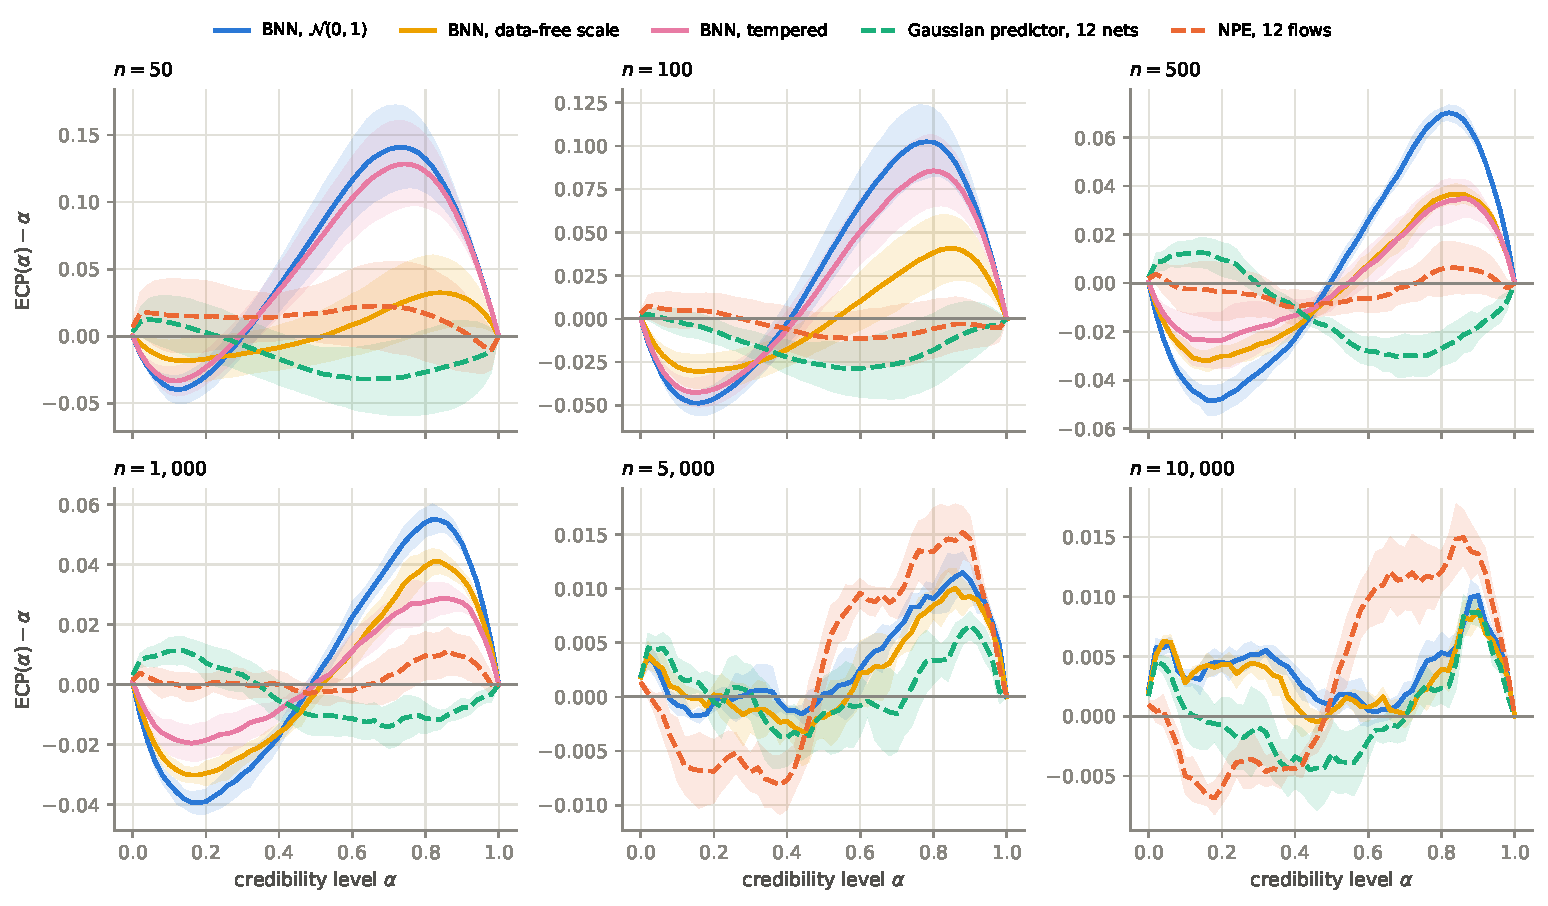
\includegraphics[width=\textwidth]{figures/project_summary/section6/tarp_ensembles.pdf}
\caption{TARP calibration of the three BNNs and the two 12-member ensembles: expected coverage minus credibility
level, $\mathrm{ECP}(\alpha)-\alpha$, against $\alpha$. 0: credible regions contain the truth as often as they claim;
above 0: conservative (too wide); below 0: over-confident. Line: pooled over repeats (20 at $n\le100$, 5 above); band:
$\pm1$ sd over the per-repeat curves. The coverage area $\int(\mathrm{ECP}(\alpha)-\alpha)\,\mathrm{d}\alpha$ at $n=50$
is $+0.052$, $+0.003$ and $+0.049$ for the $\mathcal N(0,1)$, data-free and tempered BNNs, $-0.015$ for the Gaussian
predictor and $+0.014$ for NPE.}
\label{fig:tarp_ens}
\end{figure}

\begin{table}[p]
\centering
\small\setlength{\tabcolsep}{3.5pt}
\resizebox{\textwidth}{!}{%
\begin{tabular}{lcccccc}
\toprule
 & $n=50$ & $n=100$ & $n=500$ & $n=1{,}000$ & $n=5{,}000$ & $n=10{,}000$ \\
\midrule
\inputrows{tables/understanding_results_mean.tex}
\bottomrule
\end{tabular}}
\caption{Mean error: RMS over the test datasets of (predicted mean $-$ exact posterior mean), $\sigma$ (top) and $\rho$ (bottom), bolded separately; 0 for the exact posterior. Mean $\pm$ sd over repeats (20 at $n\le100$, 5 above), same fits as Section~\ref{sec:experiments}; bold: lowest mean and every row not distinguishable from it by a two-sided paired $t$-test at $p<0.05$; $^\dagger$: the Wilcoxon test disagrees.}
\label{tab:app_mean}
\end{table}

\begin{table}[p]
\centering
\small\setlength{\tabcolsep}{3.5pt}
\resizebox{\textwidth}{!}{%
\begin{tabular}{lcccccc}
\toprule
 & $n=50$ & $n=100$ & $n=500$ & $n=1{,}000$ & $n=5{,}000$ & $n=10{,}000$ \\
\midrule
\inputrows{tables/understanding_results_sd.tex}
\bottomrule
\end{tabular}}
\caption{Width error: mean over the test datasets of $|\hat s-s^\star|/s^\star$, $\sigma$ (top) and $\rho$ (bottom), bolded separately. Too narrow scores at most 1, too wide is unbounded. Mean $\pm$ sd over repeats (20 at $n\le100$, 5 above), same fits as Section~\ref{sec:experiments}; bold: lowest mean and every row not distinguishable from it by a two-sided paired $t$-test at $p<0.05$; $^\dagger$: the Wilcoxon test disagrees.}
\label{tab:app_sd}
\end{table}

\begin{table}[p]
\centering
\small\setlength{\tabcolsep}{3.5pt}
\resizebox{\textwidth}{!}{%
\begin{tabular}{lcccccc}
\toprule
 & $n=50$ & $n=100$ & $n=500$ & $n=1{,}000$ & $n=5{,}000$ & $n=10{,}000$ \\
\midrule
\inputrows{tables/understanding_results_tarp.tex}
\bottomrule
\end{tabular}}
\caption{TARP calibration error, mean over credibility levels of $|\mathrm{ECP}(\alpha)-\alpha|$; 0 = calibrated, exact posterior 0.005. Mean $\pm$ sd over repeats (20 at $n\le100$, 5 above), same fits as Section~\ref{sec:experiments}; bold: lowest mean and every row not distinguishable from it by a two-sided paired $t$-test at $p<0.05$; $^\dagger$: the Wilcoxon test disagrees.}
\label{tab:app_tarp}
\end{table}

\subsection{Empirical Bayes and the re-tuning sampler}
\label{app:eb}
\label{sec:res_side}
Empirical Bayes (Section~\ref{sec:bnn_eb}) runs on the re-tuning sampler, and its fixed-scale control is
$\mathcal N(0,1)$ with the same re-tuning (rows in Tables~\ref{tab:paired_b} and~\ref{tab:app_mean}--\ref{tab:app_tarp}).
\textbf{Re-tuning alone} lowers the NLL of $\mathcal N(0,1)$ by 0.15 and 0.12 nats at $n=500$ and $1{,}000$ ($p\le0.002$)
and changes nothing at $n\ge5{,}000$. \textbf{Empirical Bayes} recovers the data-free scale where it is stable: its final
scale is 0.37, 0.36 and 0.32 at $n=100$, 500 and $1{,}000$, against the data-free 0.3655, and 0.32 and 0.28 at $n=5{,}000$
and $10{,}000$. Against its control it is better at $n=100$ (by 0.08 nats, $p=2\times10^{-5}$) and worse from $n=1{,}000$
(by 0.04--0.05). At $n=50$ it collapses in all 20 repeats: the scale falls to the floor of $10^{-3}$ and the network
becomes a nearly constant predictor: across test datasets its predicted width varies by at most 3.3\% (coefficient of
variation) and its predicted mean has a standard deviation of at most 12\% of the prior's. It then returns the training mean with a width of about $0.75$ times the training
standard deviation of $\theta$, a value set by $\mathrm{softplus}(0)$ because the output biases are shrunk with every
other weight, and its NLL is 0.54 nats above its control. This is the underfitting the marginal likelihood is prone to
at small $n$ \citep{lotfi2022bayesian}, and the sample-based update of the same form is reported to diverge to very small
regularizers \citep{antoran2023sampling}. A per-layer version (exploratory 3-member runs, original learning rates) did
not rescue $n=50$ and was worse than the isotropic one at $n=500$ and $1{,}000$ (by 0.09 and 0.03 nats, 0 of 5 repeats),
although \citet{mackay1992thesis} argues that one scale for all weight classes is inconsistent. Fits that dropped a failed
member without replacing it: re-tuning 10 of 20 at $n=50$, 7 of 20 at $n=100$ and 2 of the 20 at $n\ge500$; empirical
Bayes 1, 6 and 1;
every fit of the other models used all 12 members.

\section{Reproducibility}
\begingroup\raggedright
\label{app:repro}
\textbf{Code.} The code of this report is at \url{https://github.com/sam-dowd/rbf-sbi-bnn}; all paths below are relative
to it. It holds the library (\code{src/rbf\_sbi/}: simulator and exact posterior, the BNN, NPE, evaluation and
diagnostics), the scripts that build the data, tune, fit and post-process (\code{scripts/data/}, \code{scripts/tuning/},
\code{scripts/fit/}, \code{scripts/analysis/}), the scripts that regenerate every table and figure
(\code{paper/scripts/}, run in order by \code{paper/make\_paper.sh}), Slurm templates for NERSC Perlmutter
(\code{slurm/}), the canonical dataset, and the small result files the tables need (selected hyperparameters, the NLL
decomposition of Appendix~\ref{app:inside} and the convergence diagnostics of Appendix~\ref{sec:res_rhat}). The result
files of the final runs (9.2\,GB) are to be deposited separately. Each script's docstring gives its arguments.

\textbf{Environment.} Python 3.11: \code{conda create -n rbf-sbi python=3.11 pip}, \code{pip install -r requirements.txt},
which pins the versions used: \code{sklearn-contrib-bde} 1.0.2, \code{blackjax} 1.2.2 (pinned by \code{bde}),
\code{jax}/\code{jaxlib} 0.10.2, \code{flax} 0.12.8, \code{optax} 0.2.8, \code{numpy} 2.4.6, \code{scipy} 1.17.1,
\code{torch} 2.13.0, \code{nflows} 0.14, \code{scikit-optimize} 0.10.2. Hardware: Section~\ref{sec:compute}. Data, result
and scratch folders can be redirected with the environment variables \code{RBF\_SBI\_DATA}, \code{RBF\_SBI\_RESULTS}
and \code{RBF\_SBI\_SCRATCH}.

\textbf{Code version and reproduction.} Runs do not record a commit. The final runs were made between 2026-10-30 and
2026-11-05 with the project's research code; the repository is a curated copy of it whose model code differs only in
imports and paths and in the removal of a baseline that is not part of this report. Every table of this report
regenerates byte for byte from the repository's scripts and result files. GPU runs are not bit-reproducible: a re-fit
of the $\nzo$ BNN at $n=100$, repeat 0, with the repository's code reproduces its pretraining exactly up to
floating-point differences (the same stopping step for every network; test NLL of the pretrained networks $-0.669$ in
both runs), but its chains differ, and the sampled BNN's test NLL is $-0.753$ against $-0.828$ in the reported run.

\textbf{Data.} \code{python scripts/data/build\_dataset.py} writes \code{data/dataset.npz} (seed 0; 10{,}000-row pool,
1{,}000 test rows; also included in the repository). Training subsamples and fit seeds: Section~\ref{sec:datasets}.
\code{python scripts/data/build\_reference.py} computes and caches the exact test-set posteriors in
\code{data/reference\_posterior/test\_n100\_ntest1000\_seed0.npz}.

\textbf{Runs.} The BNNs, the capped Gaussian predictor and the default-budget NPE come from
\code{python scripts/fit/run\_experiment.py <key> <n> rbf\_kernel <repeats>}, submitted by
\code{slurm/submit\_final\_sweep.sh} (template \code{slurm/final\_sweep.sbatch}), which writes
\code{results/raw/final/<key>\_n<n>\_r<r>.npz}; the BNNs also write their per-draw outputs to
\code{sbi\_final\_draws/} in the scratch folder. The converged Gaussian predictor, the long-trained NPE and the NPE
variants are refits with their own scripts (Table~\ref{tab:repro}), which read and assert the seeds, subsamples and
hyperparameters of the corresponding default run.

\begin{table}[h]
\centering\footnotesize\setlength{\tabcolsep}{3pt}
\begin{tabular}{@{}>{\raggedright}p{2.35cm}l>{\raggedright\arraybackslash}p{6.4cm}@{}}
\toprule
model & result key & fitting call \\
\midrule
BNN, $\nzo$ & \code{final\_bnn\_stdnormal\_pretuned} & \code{bnn.fit\_correlated}; also writes the capped Gaussian predictor \\
BNN, data-free scale & \code{final\_bnn\_gaussprior\_pretuned} & \code{fit\_correlated}, prior $\mathcal N(0,0.3655^2)$ \\
BNN, tempered & \code{final\_bnn\_temp\_pretuned} & \code{fit\_correlated(temperature=T)}, $T$ from the search of Appendix~\ref{app:temp_search} \\
$\nzo$ + re-tune & \code{final\_bnn\_stdnormal\_retune\_pretuned} & \code{bnn.fit\_rasmussen\_gibbs\_hierarchical(}\newline\code{\ \ resample\_tau=False)} \\
empirical Bayes & \code{final\_bnn\_ebblock\_pretuned} & \code{fit\_rasmussen\_gibbs\_hierarchical(}\newline\code{\ \ resample\_tau=False, eb\_block="iso")} \\
Gaussian predictor, capped & \code{final\_bnn\_pretrained\{\_ens12,\}\_pretuned} & the $\nzo$ BNN's pretrained networks, scored unsampled \\
Gaussian predictor, converged & \code{final\_bnn\_pretrained\{\_ens12,\}\_pretuned\_long} & \code{scripts/fit/gaussian\_predictor\_long.py}\newline(\code{bnn.fit\_pretrained\_ensemble}) \\
NPE, 12 flows / 1 flow & \code{final\_npe\_ens12} / \code{final\_npe} & \code{npe.fit}, 12 member seeds \\
NPE, long-trained & \code{final\_npe\_ens12\_long} & \code{scripts/fit/npe\_long\_members.py},\newline merged by \code{scripts/fit/npe\_long\_merge.py} \\
NPE variants & \code{final\_npe\{\_ctx16,\_gauss\_ctx16\}\{\_ens12,\}} & \code{scripts/fit/npe\_variant\_members.py},\newline merged by \code{scripts/fit/npe\_variant\_merge.py} \\
\bottomrule
\end{tabular}
\caption{One row per reported model of the final runs; functions are in \code{src/rbf\_sbi/}. Hyperparameters:
Section~\ref{sec:hp} and Appendix~\ref{app:hp}. The earlier runs of Appendix~\ref{app:variants} use the sweep keys listed
in \code{scripts/fit/run\_experiment.py}'s module docstring; their result files are not released, and the code behind
their tables is in \code{legacy/}.}
\label{tab:repro}
\end{table}

\textbf{Hyperparameters.} BNN and Gaussian predictor: \code{scripts/tuning/optimize\_pretrain\_grid.py} $\to$
\code{results/hp\_search/pretrain\_grid/pretrain\_grid\_n<n>.npz}. NPE: \code{scripts/tuning/optimize\_npe.py} $\to$
\code{results/npe\_params.npz}. Temperatures: \code{scripts/tuning/optimize\_temperature\_grid.py} (with
\code{PRETUNED\_HP=1}) $\to$ \code{results/temperature\_search\_n<n>\_stdprior\_pretuned\_grid.npz}. Data-free scale:
\code{scripts/tuning/optimize\_prior\_width.py} $\to$ \code{results/gaussian\_width\_prior\_phi.npz}; its
simulation-free check \code{scripts/tuning/coherence\_width\_check.py}. All of these result files are included.

\textbf{Tables and figures,} each from a script that reads the result files and fits nothing (CPU, minutes; all run by
\code{bash paper/make\_paper.sh}):
\begin{itemize}
\item Section~\ref{sec:data}: \code{paper/scripts/rbf\_figures.py}; grid check \code{scripts/data/refine\_reference\_posterior.py}.
\item Section~\ref{sec:experiments} (Tables~\ref{tab:sec6_single} and~\ref{tab:sec6_ens}, Figures~\ref{fig:sec6_single}
  and~\ref{fig:sec6_ens}), Tables~\ref{tab:verdict}, \ref{tab:sec6_lppd}, \ref{tab:sec6_draw} and~\ref{tab:app_width}, and
  Figure~\ref{fig:tarp_ens}: \code{paper/scripts/section6.py}, after \code{scripts/analysis/lppd\_decomposition.py} has
  written \code{results/lppd\_decomposition.npz} from the per-draw outputs.
\item Tables~\ref{tab:paired_a}, \ref{tab:paired_b}, \ref{tab:npe_nll}, \ref{tab:npe_mean} and
  \ref{tab:app_mean}--\ref{tab:app_tarp}: \code{paper/scripts/appendix\_tables.py}.
\item Figure~\ref{fig:temperature_search}: \code{paper/scripts/temperature\_search\_plot.py}.
\item Table~\ref{tab:res5}: \code{scripts/analysis/chainwise\_diagnostics.py} on the per-draw outputs (one shard per model,
  \code{slurm/chainwise\_shards.sbatch}, merged by \code{scripts/analysis/merge\_chainwise\_shards.py}) $\to$
  \code{results/rbf\_chainwise\_diagnostics.npz}; then \code{paper/scripts/diagnostics\_table.py}.
\item Appendix~\ref{app:variants} (earlier runs): \code{legacy/results4\_\{scale,shape,side\}.py}.
\end{itemize}

\par\endgroup
\section{Hyperparameters and compute}
\label{app:hp}
\textbf{Hyperparameter search} (summary in Section~\ref{sec:hp}). Apart from the learning rate and weight decay, all
settings are fixed as in Sections~\ref{sec:gauss}--\ref{sec:impl}. The test set is never used.
\begin{itemize}
\item \textbf{BNN and Gaussian predictor} (\code{scripts/tuning/optimize\_pretrain\_grid.py}): one network of the BNN's
  architecture, pretrained exactly as in Section~\ref{sec:impl} and not sampled, on the training sets of repeats 0--2,
  scored by its NLL on the 1{,}000 pool rows that follow the training rows (at $n=10{,}000$, where the pool has no rows
  left, on an inner 80/20 split of the training rows). Grid of 17 learning rates ($10^{-5}$ to $10^{-1}$, quarter decades)
  by 15 weight decays ($10^{-7}$ to 1, half decades); the argmin of the mean over the three training sets is used at
  every size. One pair per size serves every BNN variant and both versions of the Gaussian predictor.
\item \textbf{NPE} (\code{scripts/tuning/optimize\_npe.py}): Bayesian optimization (Section~\ref{sec:hp}) of the early-stopping
  validation NLL on an 80/20 split (seed 123) of the repeat-0 training rows; 200\,s per size, 3--20 trials (3, 5, 9,
  14, 20 and 19 at $n=10{,}000$, 5{,}000, 1{,}000, 500, 100 and 50).
\end{itemize}

\textbf{Rationale.} Only learning rate and weight decay are searched, with the architecture fixed and
identical across methods, so that a difference between methods cannot come from one of them receiving a
larger or better-tuned network. MILE's sampler settings are not searched: in the MILE ablations (two UCI
regression datasets, bikesharing and protein) predictive performance changes little with the energy-variance schedule or the two
parameters of the step-size adaptation, and only marginally with a much longer warmup, which its authors
judge not worth the linear cost; they call the method ``effectively tuning-free'' \citep{sommer2025mile}. In MILE the
two hyperparameters act only on the pretraining that initializes the chains and on the initial step size, so the
BNN's network is scored as a standalone predictor, on a grid so that the whole landscape is visible. The grid
supersedes an earlier search that scored complete 3-member MILE fits by held-out NLL (\code{legacy/optimize\_bde.py};
12--15 trials per size at $n\le1{,}000$, and 29--30 with a single-split objective at $n\ge5{,}000$), whose values the
earlier runs of Appendix~\ref{app:variants} use. Moving from those values to the grid's left the sampled BNNs
essentially unchanged (paired test-NLL differences of $+0.001$ to $+0.021$ nats for $\nzo$ and the data-free scale at
every $n$, each smaller than its sd) and improved the Gaussian predictor where the earlier values had under-trained it.
NPE keeps its own search; the baselines were not re-tuned with the BNN's objective. The reasons for the following were
not recorded: (a) NPE's search ranges; (b) its random state and 10 initial points (the \code{scikit-optimize} default);
(c) its 200\,s budget; (d) the choice of 3 training draws and 1{,}000 held-out rows for the grid, taken over from the
earlier BNN search.

\textbf{Differences between the searches.} (i) NPE's search was in effect a random search of 3--10 points.
\code{scikit-optimize} draws 10 random points before its Gaussian-process phase. At $n\ge1{,}000$ the 200\,s budget
ended within them (3, 5 and 9 trials); at $n\le500$ the 4--10 guided trials that followed did not improve on them, so
every selected pair is one of the random initial points (checked by regenerating them from the random state). (ii) The objectives differ: the BNN's network is scored on 1{,}000
held-out points over three training draws, NPE on 20\% of one draw (10 points at $n=50$).

\textbf{Shared by all BNNs.} $100\to16\to16\to16\to5$, soft-sign, $d=2{,}245$. Pretraining: AdamW at the per-size
learning rate and weight decay of Table~\ref{tab:hp}, full batch, 80/20 split, validation NLL every 100 steps,
patience 5 evaluations ($\Delta>10^{-4}$), at least 500 and at most 2{,}000 steps, best checkpoint kept.
MILE: 50{,}000 warmup steps (phases I--III $40{,}000/5{,}000/5{,}000$), EEVPD target $0.5\to0.1$, ESS target 100,
initial step size equal to the learning rate; 10{,}000 sampling steps thinned by 10 to 1{,}000 kept draws per
member; $K=12$ members; under stock MILE, at most three attempts in all (the original seed and two re-seeds) to
replace non-finite members. Gaussian
predictor and NPE: Sections~\ref{sec:gauss} and~\ref{sec:npe}.

\begin{table}[h]
\centering\footnotesize\setlength{\tabcolsep}{4pt}
\begin{tabular}{@{}>{\raggedright}p{2.4cm}>{\raggedright}p{2.3cm}l>{\raggedright}p{2.8cm}>{\raggedright}p{1.9cm}>{\raggedright\arraybackslash}p{2.6cm}@{}}
\toprule
model & prior & $T$ & sampling loop & steps / kept per member & wall time per fit \\
\midrule
$\nzo$ & $\nzo$ & 1 & stock MILE & 10{,}000 / 1{,}000 & 37--71\,s \\
tempered & $\nzo$ & 0.7 / 0.7 / 0.6 / 0.7 & stock MILE, tempered warmup & 10{,}000 / 1{,}000 & 36--55\,s \\
data-free scale & $\mathcal N(0,0.3655^2)$ & 1 & stock MILE & 10{,}000 / 1{,}000 & 36--72\,s \\
$\nzo$ + re-tune & $\nzo$ & 1 & re-tune every 1{,}000 steps & 12{,}500 / 1{,}000 & 422--534\,s \\
empirical Bayes & $\mathcal N(0,\tau^2)$, block update & 1 & re-tune loop & 12{,}500 / 1{,}000 & 411--527\,s \\
Gaussian predictor, converged & -- & -- & AdamW, $\le200{,}000$ steps & -- & 24--82\,s \\
NPE, 12 flows & -- & -- & Adam, $\le20{,}000$ steps & -- & 157--238\,s ($n\le1{,}000$); 663--907\,s ($n\ge5{,}000$) \\
\bottomrule
\end{tabular}
\caption{Per-model settings and wall time per fit (one training set, all 12 members, fitting and prediction; median per
size, range over sizes) of the final runs, on one NVIDIA A100 (Section~\ref{sec:compute}). BNN and Gaussian-predictor
times are recorded in each result file; NPE times are job wall times from the run log (not included in the repository) divided by the
repeats per job. Re-tune: 200 step-size and 50 $L$ steps every 100 kept draws, 2{,}500 extra steps per member.
Empirical-Bayes update: Section~\ref{sec:bnn_eb}.}
\label{tab:compute}
\end{table}

\textbf{Temperature search.}
\label{app:temp_search}
The temperatures of the tempered BNN ($T=0.7$, $0.7$, $0.6$, $0.7$ at $n=50$--$1{,}000$; Section~\ref{sec:bnn_temp})
are chosen as follows. The MCLMC target is $\log p(\mathbf w)+\tfrac1T\log p(\mathcal D\mid\mathbf w)$ under the
$\mathcal N(0,1)$ prior, with the pretraining-tuned learning rate and weight decay. $T$ is searched per size on the grid
$0.2, 0.3, \dots, 1.0$ by bisection on the sign of the local slope, always including $T=1$, so 5 of the 9 grid points
are evaluated. Each evaluated $T$ is a 3-member fit on the training sets of repeats 0--2, scored by the NLL on the
1{,}000 pool rows that follow each repeat's training rows; the chosen $T$ minimizes the mean over the three repeats,
over every evaluated point, with no filter on mixing.

The gain over $T=1$ at the chosen $T$ is 0.08, 0.20, 0.21 and 0.11 nats on validation at $n=50$, 100, 500 and
1{,}000; in the final 12-member runs on the test set it is 0.06, 0.10, 0.25 and 0.15 nats. At $n\le100$ the
validation NLL is flat to within the repeat spread between $T=0.6$ and $0.8$, and almost every evaluated $T$ mixes (one repeat at $n=100$, $T=0.9$, has a
maximum split-$\widehat R$ of 1.53). At
$n=500$ and $1{,}000$ the minimum lies next to a mixing failure: at $n=500$, $T=0.5$ has $\widehat R$ 2.9--10.3 and
$T=0.4$ diverges (validation NLL $+598$, $\widehat R\approx100$); at $n=1{,}000$, $T=0.6$ has $\widehat R$ 1.9--6.8
and a higher mean NLL than $T=0.7$ ($-1.67$ against $-1.91$): its two worst-mixed repeats ($\widehat R$ 5.2, 6.8)
score $-1.52$ and $-1.53$, while the third ($\widehat R$ 1.85) scores $-1.95$, the lowest single value at that size.
The chosen $T$ is therefore the coldest temperature at which the chains still mix, not an interior optimum of a
smooth curve, at the two sizes where tempering helps most (Figure~\ref{fig:temperature_search}).

\begin{figure}[h]
\centering
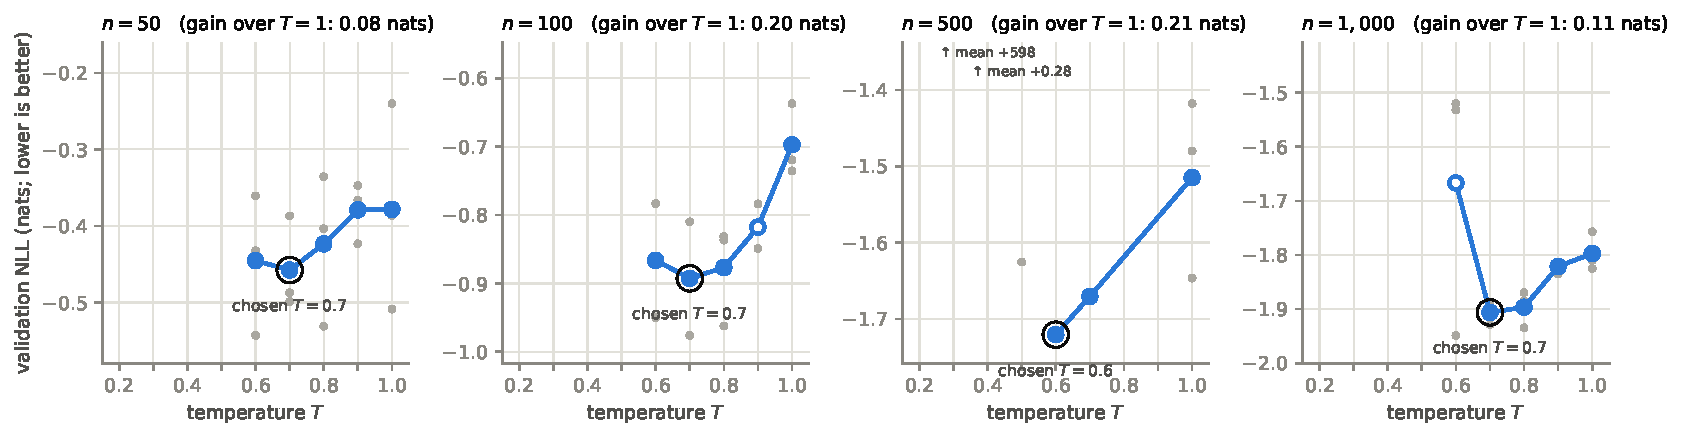
\includegraphics[width=\linewidth]{figures/understanding_results/temperature_search.pdf}
\caption{Validation NLL against temperature from the search behind the tempered BNN. Line and filled markers: mean
over repeats 0--2 (3-member fits, $\mathcal N(0,1)$ prior, pretraining-tuned lr/wd); grey dots: each repeat;
ring: the chosen $T$. Open markers: max split-$\widehat R$ on the predicted mean $>1.5$ in at least one repeat
(poorly mixed; at $n=100$, $T=0.9$ is flagged by one repeat at 1.53). Means above the panel are written at its top
edge; repeats above it are not drawn (all three at $n=500$, $T=0.4$; two of three at $n=500$, $T=0.5$); every other
value is in range. Only the evaluated temperatures are shown (bisection, 5 of 9 grid points per size). Each panel has
its own vertical scale. Each panel's title gives the chosen $T$ and its mean gain over $T=1$ on validation.}
\label{fig:temperature_search}
\end{figure}
\repro{search \code{scripts/tuning/optimize\_temperature\_grid.py} $\to$
\code{results/temperature\_search\_n<n>\_stdprior\_pretuned\_grid.npz} ($n=50$, 100, 500, 1{,}000); figure
\code{python paper/scripts/temperature\_search\_plot.py}.}

\section{Implementation of the correlated \texttt{bde} model}
\begingroup\raggedright
\label{app:bde}
\label{app:impl}
\textbf{Departures from stock \code{bde}}, all subclass overrides in \code{src/rbf\_sbi/bnn.py} (installed package unmodified):
\begin{itemize}
\item \textbf{Correlated two-target head.} \code{bde} is single-output: its output width is fixed at 2 and its
  sampling likelihood is a univariate Gaussian whatever loss is passed. A joint $(\sigma,\rho)$ likelihood with a
  fitted correlation needs four overrides (output width, log-posterior, pretraining loss, and \code{fit} itself
  to bypass a check on the loss class) plus an sklearn-tag override; details below.
\item \textbf{Pretraining schedule.} \code{bde} checks the validation loss at every step, so its patience counts
  steps; at $n=100$ pretraining stopped almost immediately. We evaluate every 100 steps, stop after 5
  evaluations without improvement ($>10^{-4}$), never before step 500, and cap at 2{,}000 steps; full-batch,
  80/20 split of the training set. AdamW replaces \code{bde}'s Adam, which ignored weight decay. Learning rate
  and weight decay are tuned per size (Section~\ref{sec:hp}).
\item \textbf{Member retry} (stock MILE). Members whose chains become non-finite are discarded; the whole ensemble
  is refitted with a new seed on the same training rows, and finite members are pooled across attempts until $K$
  exist, for at most three attempts in all; the failure rate is recorded. The re-tuning loop has no retry: a
  non-finite member is dropped (Section~\ref{sec:convdiag}).
\item \textbf{Tempering} (Section~\ref{sec:bnn_temp}): $\log p(\mathbf w)+\log p(\mathcal{D}\mid\mathbf w)/T$
  in warmup and sampling; pretraining is untouched.
\item \textbf{Periodic re-tuning} (optional; Appendix~\ref{sec:retune}): after every 100 kept draws (1{,}000
  steps) the chain re-estimates $\epsilon$ (200 steps) and $L$ (50 steps) at the final EEVPD target 0.1, starting
  from the current values and carrying the step-size adaptation's running averages across re-tunes; 2{,}500 extra
  steps per chain. This re-implements \code{bde}'s phase I/II loop, which otherwise resets its accumulators on
  every call.
\end{itemize}

\textbf{The two-target head.} \code{bde}'s \code{BdeRegressor} is single-output: its sklearn tags declare \code{single\_output=True}, its
network has two outputs (mean and scale), and its sampling likelihood slices a univariate Gaussian from them
whatever loss is passed. \code{CorrelatedBdeRegressor} (\code{src/rbf\_sbi/bnn.py}) subclasses it; the installed package is
not modified.
\begin{enumerate}
\item \textbf{Output width.} \code{\_CorrelatedBdeBuilder.\_determine\_output\_dim} returns 5
  ($\mu_\sigma,\mu_\rho,a_\sigma,a_\rho,c$) instead of 2.
\item \textbf{Log-posterior.} \code{\_build\_log\_post} returns \code{\_BivariateProbabilisticModel}, whose
  \code{log\_likelihood} is the bivariate normal of Eq.~\eqref{eq:biv} summed over the training set
  (\code{softplus}$+10^{-6}$ scales, $\tanh$ correlation) and whose \code{log\_unnormalized\_posterior} is
  $\log p(\mathbf w)+\log p(\mathcal D\mid\mathbf w)/T$.
\item \textbf{Pretraining loss.} \code{BivariateGaussianNLL}, the negative of the same log density, summed (not
  averaged) over the batch so that pretraining and sampling share one scale.
\item \textbf{\code{fit}.} \code{Bde.\_fit} calls \code{task.validate\_loss}, which accepts only the loss classes
  \code{GaussianNLL} and \code{Rmse} for regression, by class identity. \code{CorrelatedBdeRegressor.fit} is a copy of
  \code{Bde.\_fit} without that check, plus the pretraining schedule of Section~\ref{sec:impl} (evaluation every 100
  steps, minimum 500 steps via \code{\_MinStepsEarlyStoppingCallback}, \code{optax.adamw}).
\item \textbf{sklearn tags.} \code{\_\_sklearn\_tags\_\_} declares \code{multi\_output=True}, \code{single\_output=False},
  \code{two\_d\_labels=True}; otherwise \code{bde.data.utils.validate\_fit\_data} treats a two-column target as a
  column vector and keeps only the first column, without an error.
\end{enumerate}
\textbf{The method-resolution-order (MRO) pitfall.} Overriding \code{\_fit} instead of \code{fit} does nothing: \code{BdeRegressor.fit} calls
\code{super().\_fit}, and that \code{super()} is bound to \code{BdeRegressor}, so it resolves to \code{Bde.\_fit}
whatever a subclass defines. The first implementation did this and failed with ``\code{BivariateGaussianNLL} not
allowed for task regression''.

\textbf{Read-out.} Scales are read out through the same $\mathrm{softplus}(\cdot)+10^{-6}$ map as in the likelihood,
then multiplied by the training-set target standard deviation; means are destandardized. The correlation needs no
transformation: $\mathrm{Corr}(aX+b,\,cY+d)=\mathrm{Corr}(X,Y)$ for $a,c>0$.

\textbf{Later additions} (same file): \code{\_draw\_samples} (a kept-sample count independent of the thinning
factor), member-by-member prediction (\code{\_predict\_raw\_per\_member}, identical output at a third of the GPU
memory), and the re-tune loop \code{fit\_rasmussen\_gibbs\_hierarchical}, which runs its own MCLMC chain on the same
log-posterior. All rely on undocumented \code{bde} internals and are tied to version 1.0.2.

\par\endgroup
\section{Background details}
\label{app:bg}
\subsection{Microcanonical Langevin Monte Carlo}
\label{sec:mclmc}
MCLMC \citep{robnik2024mclmc} samples a target $p(\mathbf w\mid\mathcal{D})$ on $\mathbb{R}^d$ with a
unit-speed velocity $\mathbf{u}$ ($\lVert\mathbf{u}\rVert=1$) and the dynamics, in the form used by
\citet{sommer2025mile},
\begin{equation}
\label{eq:mclmc}
\mathrm{d}\mathbf w=\mathbf{u}\,\mathrm{d}t,\qquad
\mathrm{d}\mathbf{u}=\big(I-\mathbf{u}\mathbf{u}^\top\big)\Big(\tfrac{1}{d-1}\nabla\log p(\mathbf w\mid\mathcal{D})\,\mathrm{d}t
+\xi\,\mathrm{d}\mathbf{W}\Big).
\end{equation}
The stationary distribution of $\mathbf w$ is the target for any noise level $\xi$, including the
deterministic dynamics $\xi=0$ \citep{robnik2024mclmc}; the noise only decorrelates the velocity, over a
length $L$. In practice the deterministic part is integrated with the minimal-norm integrator (two gradient
evaluations per step of size $\epsilon$), and the noise is applied as a partial refresh of the velocity
\citep{robnik2024mclmc},
\begin{equation}
\mathbf{u}\leftarrow\frac{\mathbf{u}+\omega\mathbf{z}}{\lVert\mathbf{u}+\omega\mathbf{z}\rVert},\qquad
\mathbf{z}\sim\mathcal{N}(0,I),\qquad \omega=\sqrt{\big(e^{2\epsilon/L}-1\big)/d},
\end{equation}
with $\omega$ as implemented in BlackJAX \citep{cabezas2024blackjax}. There is no Metropolis--Hastings
correction, so a finite $\epsilon$ biases the stationary distribution. The bias is controlled by tuning
$\epsilon$ to a target energy-error variance per dimension (EEVPD), $\mathrm{Var}[\Delta E]/d$
\citep{robnik2023mchmc}; the BlackJAX update uses $\mathrm{Var}[\Delta E]\propto\epsilon^6$. Tuning
proceeds in three phases \citep{sommer2025mile}: (I) adapt $\epsilon$ to the target EEVPD while burning
in; (II) set $L=\big(\sum_i\mathrm{Var}[w_i]\big)^{1/2}$ from the chain's own variance; (III) refine
$L=c\,\epsilon\,N/\widehat{\mathrm{ESS}}$ from the effective sample size of $N$ further steps
($c=0.4$ in the implementation used here).

\subsection{Tempering}
\label{app:bg_tempering}
\citet[App.~E]{wenzel2020cold} also show
that the KL-weighted evidence lower bound used in variational BNNs,
$\lambda\,\mathrm{KL}\big(q(\mathbf w)\,\|\,p(\mathbf w)\big)-\sum_i\mathbb{E}_q\log p(y_i\mid x_i,\mathbf w)$, has the same
minimizer as $\mathrm{KL}(q\,\|\,p_P)$ with $T=\lambda$: down-weighting the KL term ($\lambda<1$) is variational
inference for the partially tempered posterior. The temperature-weighted objective of
\citet{delaunoy2024lowbudget} is of this kind. This project uses partial tempering, Eq.~\eqref{eq:partial}.

\textbf{Tempering versus changing the prior.} The prior factor of full tempering is itself a prior: for a Gaussian
prior, $\mathcal{N}(\mathbf w;0,s^2I)^{1/T}\propto\mathcal{N}(\mathbf w;0,Ts^2I)$ \citep[Sec.~2.2]{wenzel2020cold}, so full
tempering at $T$ with prior $\mathcal{N}(0,s^2)$ is exactly partial tempering at $T$ with prior $\mathcal{N}(0,Ts^2)$; the two
schemes differ only by a rescaling of the prior. The likelihood factor $p(\mathcal{D}\mid\mathbf w)^{1/T}$, which both
contain and which is all of partial tempering, cannot be obtained by changing the prior. Writing the partially
tempered posterior as a $T=1$ posterior, $p(\mathcal{D}\mid\mathbf w)\,\tilde p(\mathbf w)$, requires
$\tilde p(\mathbf w)\propto p(\mathbf w)\,p(\mathcal{D}\mid\mathbf w)^{1/T-1}$, which depends on the training data and is
therefore not a prior. Any prior, of any scale or shape, can at most approximate the effect of likelihood tempering,
never reproduce it; Eq.~\eqref{eq:tempered_obs} shows the effect is a change of the likelihood instead.

\textbf{Where the temperature acts.} Only in the MCLMC target, during warmup and sampling. Pretraining (the
deep-ensemble optimization that initializes the chains) uses the untempered likelihood. Prediction and evaluation
are untempered: each posterior draw $\mathbf w_{ks}$ predicts with its own Gaussian
$\mathcal{N}_2(\theta;\boldsymbol\mu_{ks}(S),\Sigma_{ks}(S))$, and the predictive is the mixture of
Section~\ref{sec:metrics}, exactly as at $T=1$. Tempering changes which weights are drawn, not how a drawn network
predicts, so the test NLL of a tempered BNN is a density of the same form as that of the untempered BNN and of NPE,
and the three are directly comparable.

\subsection{Empirical Bayes and data-free calibration of the prior scale}
\label{app:bg_eb}
No prior reproduces likelihood tempering (Section~\ref{sec:bg_tempering}). The alternative considered here keeps
$T=1$ and sets the scale of an isotropic Gaussian prior, either from the training data or from the simulator alone.

\textbf{Empirical Bayes (type-II maximum likelihood).} Make the prior scale a hyperparameter,
$p(\mathbf w\mid\tau)=\mathcal{N}(\mathbf w;0,\tau^2 I_d)$, and choose it to maximize the evidence
\begin{equation}
p(\mathcal{D}\mid\tau)=\int p(\mathcal{D}\mid\mathbf w)\,p(\mathbf w\mid\tau)\,\mathrm{d}\mathbf w,\qquad
\hat\tau=\arg\max_\tau\,p(\mathcal{D}\mid\tau),
\end{equation}
then use the posterior $p(\mathbf w\mid\mathcal{D},\hat\tau)$ \citep{mackay1992practical}. Since
$\partial_\tau\log p(\mathcal{D}\mid\tau)=\mathbb{E}_{p(\mathbf w\mid\mathcal{D},\tau)}\big[\partial_\tau\log p(\mathbf w\mid\tau)\big]$
and $\partial_\tau\log p(\mathbf w\mid\tau)=-d/\tau+\lVert\mathbf w\rVert^2/\tau^3$, the evidence is stationary where
\begin{equation}
\label{eq:eb_fixed_point}
\hat\tau^2=\frac{\mathbb{E}_{p(\mathbf w\mid\mathcal{D},\hat\tau)}\lVert\mathbf w\rVert^2}{d}
=\frac{\lVert\mathbf m\rVert^2}{\gamma},\qquad
\gamma=d-\frac{\operatorname{tr}\mathrm{Cov}[\mathbf w\mid\mathcal{D},\hat\tau]}{\hat\tau^2},
\end{equation}
with $\mathbf m$ the posterior mean. The second form is MacKay's evidence condition
$2\alpha E_W^{\mathrm{MP}}=k-\alpha\operatorname{Tr}\!A^{-1}$ with $\alpha=1/\tau^2$
\citep[Eqs.~2.22--2.23]{mackay1992thesis}, where $\gamma\in[0,d]$ is ``the number of good parameter measurements'',
the effective number of weights determined by the data. MacKay evaluates it at the posterior mode with the
Gaussian (Laplace) covariance $A^{-1}$, which is exact only for quadratic energies; with posterior samples, as here,
Eq.~\eqref{eq:eb_fixed_point} can be used with sampled moments and iterated as a fixed point. Two caveats: the data
are used twice, once to choose $\tau$ and once in the posterior; and if $\gamma$ is small (little data relative to
$d$), the fixed point is poorly determined.

\textbf{Data-free calibration.} Alternatively, the prior can be chosen before any training data are seen, so that
the network's prior predictive is consistent with the simulator. \citet{delaunoy2024lowbudget} optimize a per-weight
prior so that the BNN's prior predictive matches a calibrated target; the simplest version, used here, chooses the
single scale $\tau$ for which the prior predictive's coverage of the simulator's parameters is calibrated
(Section~\ref{sec:bnn_datafree}). Both routes fit the prior predictive to the simulator's joint distribution of
$(\theta,S)$, one through the evidence of the training sample and one through coverage without data. In a
well-specified model they should therefore select the same scale at every $n$, and a scale that drifts with $n$
indicates that no single prior of this family reproduces the simulator. Agreement at some $n$ therefore shows that the
scale is right for this family, not that the family is right: an isotropic Gaussian with the correct scale can still be
the wrong form of prior. This is our expectation rather than a
published result; Appendices~\ref{app:eb} and~\ref{sec:res_scale} test it.

\section{Reference posterior and NLL details}
\label{app:ref}
\textbf{Grid adequacy.} On the global grid two test datasets (true $\rho=0.049$, the smallest in the test set,
and $0.062$) put 1.5\% and 4.7\% of their mass in the lowest $\rho$ cell, and 40 have a $\rho$ posterior
narrower than two cells. Re-evaluating every test posterior on a per-dataset $300\times300$ grid over
$\pm10$ posterior standard deviations (float64, $\rho$ down to $10^{-3}$, exact density at $\theta^*$) leaves
the summaries unchanged: the ratio of fine to coarse posterior standard deviation has median 1.0000 for both
parameters, the posterior correlation and calibration agree to three decimals, and the mean reference test NLL
moves by 0.002 nats. Only the two boundary datasets change materially: 3.8\% and 11\% of their mass lies below
$\rho=0.02$, and their $\rho$ standard deviation is 24\% and 30\% larger. The tail is genuine. With grid
spacing $1/9$ the correlation between neighbouring points, $\exp(-1/(162\rho^2))$, is below $10^{-3}$ for
$\rho<0.03$, so the likelihood is flat in $\rho$ there and the posterior follows the prior towards
$\rho=0$. The global grid is used throughout; quantities that depend on it are insensitive to this choice
(e.g.\ the per-dataset ratio of the BNN's width to its warranted width, Section~\ref{sec:anatomy}, is unchanged to three
decimals).

\textbf{Per-method densities.} Each method's $q$ is a normalized
density on $\theta$ in original units, evaluated exactly at $\theta^\ast_j$:
\begin{itemize}
\item \emph{Gaussian predictor}: the equal-weight mixture of its 12 networks' Gaussians (one Gaussian for a single
  network), each from Eq.~\eqref{eq:biv} after mapping the network's outputs back to original units as for
  the BNN below; for one Gaussian,
  $-\log q=\log(2\pi)+\log s_\sigma+\log s_\rho+\tfrac12\log(1-r^2)+\tfrac{1}{2(1-r^2)}\big(z_\sigma^2+z_\rho^2-2rz_\sigma z_\rho\big)$
  with $z_p=(\theta_p-\mu_p)/s_p$.
\item \emph{BNN}: the equal-weight mixture over all $KS$ posterior draws,
  \begin{equation}
  q(\theta\mid S)=\frac{1}{KS}\sum_{k=1}^{K}\sum_{s=1}^{S}\mathcal{N}_2\big(\theta;\,\boldsymbol\mu_{ks}(S),\,\Sigma_{ks}(S)\big),
  \end{equation}
  each component from Eq.~\eqref{eq:biv} after mapping the draw's outputs back to original units
  ($\boldsymbol\mu\mapsto\boldsymbol\mu\odot\mathbf s_y+\mathbf m_y$, $s_\bullet\mapsto s_\bullet s_{y,\bullet}$, $r$
  unchanged), so no Jacobian term arises. Evaluated as $\operatorname{logsumexp}$ over components minus $\log(KS)$.
\item \emph{NPE}: by change of variables, $\log q_\phi(\theta\mid S)=\log\mathcal{N}\big(\Psi(\theta);0,I_2\big)+
  \log\lvert\det\partial \Psi/\partial\theta\rvert$, where $\Psi$ maps $\theta$ to the base variable through two masked
  affine autoregressive layers, each followed by an order reversal (Jacobian determinant 1). Each layer sets
  $y_i=a_i x_i+b_i$, with $a_i=\mathrm{softplus}(\cdot)+10^{-3}$ and $b_i$ functions of $x_{<i}$ and $g(S)$,
  contributing $\sum_i\log a_i$.
\item \emph{Ensembles} of the baselines: $\log\frac1K\sum_k q_k(\theta^\ast\mid S)$ over the members.
\item \emph{Exact posterior}: the grid density at $\theta^\ast$ (grid mass per cell divided by the cell area,
  bilinearly interpolated).
\end{itemize}
Because all five are densities on the same space in the same units, their NLLs are directly comparable.

\section{Further prior and sampler variants}
\label{app:variants}
All results in this appendix come from earlier 3-member runs: 5 repeats per size, the earlier BNN hyperparameters of
Appendix~\ref{app:hp}, NPE as a single flow, and temperatures 0.2 / 0.3 / 0.6 / 0.8 for the tempered BNN. They are not
comparable number for number with Section~\ref{sec:experiments}, and are kept for the variants not run in the final
runs and for two checks of the prior scale.

\subsection{Prior scale: data-free width and empirical Bayes}
\label{sec:res_scale}
\label{app:scale}
The final results of both are in Section~\ref{sec:res_ens} and Appendix~\ref{app:eb}; this appendix gives the
methods and, from the earlier runs, two checks of the evidence's fixed point.

Both models replace $\mathcal{N}(0,1)$ by an isotropic $\mathcal{N}(0,\tau^2)$ (Section~\ref{sec:bg_eb}).

\emph{Data-free width.} $\tau=0.3655$, chosen before any training by Gaussian-process Bayesian optimization of
$|\text{coverage area}|$ of the prior predictive: weights drawn from $\mathcal{N}(0,\tau^2)$, the untrained network's predictive
evaluated by TARP (Appendix~\ref{app:moments}) on fresh simulator draws, with inputs standardized by a simulator-drawn
measurement set and $\theta$ by the prior moments. The width minimizing $|\text{coverage area}|$ gives $+0.0037$, against $+0.200$ for
$\mathcal{N}(0,1)$. It is a continuous version of the fixed-width sweep of \citet[Fig.~1]{delaunoy2024lowbudget}. Run on stock MILE,
paired with $\mathcal{N}(0,1)$. At fit time the BNN standardizes with training-set statistics, so at small $n$ the width
acts in slightly different units from those it was calibrated in.

\emph{Empirical Bayes.} One scale for all weights, updated between blocks inside the re-tune loop
(Section~\ref{sec:bnn_eb}). Each member starts at the RMS of its pretrained weights; the scale is fixed for the
one-time warmup and within each 1{,}000-step block. After a block, the target $\tau_{\text{t}}^2=\lVert\mathbf m\rVert^2/\gamma$ of
Eq.~\eqref{eq:eb_fixed_point} is computed from the block's per-weight mean $\mathbf m$ and variance, with $\gamma$ clamped
to $[1,d]$; $\log\tau$ moves half-way towards $\log\tau_{\text{t}}$, by at most a factor 2, with a floor of $10^{-3}$, and
$(L,\epsilon)$ are re-tuned. All kept draws are retained, including those of early blocks drawn under a scale still moving.
Paired with $\mathcal{N}(0,1)$ plus the same re-tune.

\begin{table}[h]
\centering\small
\begin{adjustbox}{max width=\textwidth}
\begin{tabular}{rccccHHHHH}
\toprule
\multicolumn{5}{l}{\textit{(a) data-free width vs.\ $\mathcal{N}(0,1)$ (stock MILE)}} &&&&& \\
$n$ & test NLL & paired & width / warranted & RMS aleatoric &&&&& \\
 & & difference & $\sigma$/$\rho$ & $\sigma$/$\rho$ &&&&& \\
\midrule
\inputrows{tables/results4_scale.tex}
\bottomrule
\end{tabular}
\end{adjustbox}

\vspace{0.8em}
\begin{adjustbox}{max width=\textwidth}
\begin{tabular}{rHHHH>{\hspace{2\tabcolsep}}ccccc}
\toprule
\multicolumn{10}{l}{\textit{(b) empirical Bayes vs.\ $\mathcal{N}(0,1)$ + re-tune}} \\
$n$ &&&&& test NLL & paired & width / warranted & RMS aleatoric & empirical-Bayes scale \\
 &&&&& & difference & $\sigma$/$\rho$ & $\sigma$/$\rho$ & median (at floor) \\
\midrule
\inputrows{tables/results4_scale.tex}
\bottomrule
\end{tabular}
\end{adjustbox}
\caption{Prior-scale models against their controls ($\to$: control, then model; means over 5 repeats). Paired difference: model
minus control ($k$/5: model better). Bold: the better of each pair (both if within the sd of their paired difference); width
/ warranted closer to 1, RMS aleatoric closer to the exact sd (0.153 / 0.054). Empirical-Bayes scale: median final scale over 15 members
(5 repeats $\times$ 3), with the number at the $10^{-3}$ floor ($<0.01$).}
\label{tab:res4_scale}
\end{table}

\begin{itemize}
\item \textbf{Empirical Bayes recovers the data-free width at $n=100$--$1{,}000$.} The median final scale is 0.378, 0.350 and
  0.324 (ranges 0.32--0.39, 0.34--0.36, 0.31--0.33), within 11\% of 0.3655. Two independent checks place the evidence's
  fixed point within $\sim$10\% of 0.3655 at these sizes: the zero-data one-point evidence peaks at 0.3655 in 5/5 repeats,
  and fixed-width chains satisfy the stationarity condition of Eq.~\eqref{eq:eb_fixed_point} at 0.382, 0.373 and 0.400. The
  data-chosen and the data-free scales therefore agree, so the scale is well specified: for an isotropic Gaussian
  prior on this task the right scale is about 0.37, not MILE's default of 1 (Section~\ref{sec:bg_eb}). This does not
  make the isotropic Gaussian form well specified. The empirical-Bayes scale drifts at larger $n$ (0.32 and 0.28 at
  $n=5{,}000$ and $10{,}000$ in the final runs, Appendix~\ref{app:eb}), and at intermediate $n$, where the form rather
  than the scale dominates, tempering gains more than the correct scale does (Section~\ref{sec:disc_adjust}).
\end{itemize}

\subsection{Prior shape, and our claim on priors versus tempering}
\label{sec:res_shape}
$\nzo$ is replaced by a Student-$t$ with $\nu=4$ and scale $s=1/\sqrt2$ on every weight, on stock MILE with the same
chain budget, seeds, subsamples and hyperparameters. Its variance $s^2\nu/(\nu-2)=1$ equals that of $\nzo$, so the
pair differs in tail shape only. It is the marginal of $w\mid\tau^2\sim\mathcal N(0,\tau^2)$,
$\tau^2\sim\text{Inv-Gamma}(2,1)$, the weight prior of the Gibbs variants (Appendix~\ref{sec:res_other}). Heavy tails are
also what the pretrained weights show: by the Akaike information criterion (AIC) a Student-$t$ fits the AdamW-pretrained weights better than a Laplace or a
Gaussian at $n=100$ and $n=10{,}000$ (fitted $\nu=3.4$ and $3.0$).

\begin{table}[h]
\centering
\resizebox{\textwidth}{!}{%
\begin{tabular}{rcccccc}
\toprule
 & test NLL & paired & width / warranted & RMS aleatoric & RMS epistemic & $\max\widehat R$ \\
$n$ & $\nzo\to$ Student-$t$ & difference & $\sigma$/$\rho$ & $\sigma$/$\rho$ & $\sigma$/$\rho$ & range \\
\midrule
\inputrows{tables/results4_shape.tex}
\bottomrule
\end{tabular}}
\caption{Student-$t(4,1/\sqrt2)$ against $\nzo$, both on stock MILE ($\to$: $\nzo$ value, then Student-$t$; means over 5
repeats). Paired difference: Student-$t$ minus $\nzo$ ($k$/5: Student-$t$ better). Bold: paired
difference with $|\text{mean}|>\text{sd}$ and the same sign on 5 of 5 repeats.}
\label{tab:res4_shape}
\end{table}

\begin{itemize}
\item \textbf{NLL.} Student-$t$ is better at $n=50$ ($-0.098\pm0.035$, 5/5) and $n=1{,}000$ ($-0.067\pm0.054$, 5/5); there is
  no difference at $n=100$ and 500 ($+0.034\pm0.111$, $+0.026\pm0.088$; 1/5 each) or from $n=5{,}000$ ($|\Delta|\le0.004$).
\item \textbf{Widths.} Width over warranted width and RMS aleatoric width change by less than their paired sd at every
  $n\le1{,}000$, and by at most 0.005 above (at $n=50$, 2.20 / 2.34 to 2.27 / 2.24). The RMS epistemic width falls by 4--10\% at $n\le100$, about one paired sd. The
  shape of the prior does not touch the excess width of Section~\ref{sec:anatomy}.
\item \textbf{Where the gains sit.} With a Gaussian summary of each predictive (its first two moments and correlation): at $n=50$ the summary NLL
  changes by $-0.032\pm0.072$ (3/5) against $-0.098\pm0.035$ for the actual NLL, so the gain is in the shape of the
  predictive mixture; at $n=1{,}000$ the summary carries all of it ($-0.066\pm0.064$), i.e.\ the first two moments and the
  correlation.
\item \textbf{Against the other remedies} (paired, all stock MILE). At $n=50$ the data-free width is better than Student-$t$ by
  $0.140\pm0.062$ (5/5); tempering and Student-$t$ are indistinguishable ($0.039\pm0.278$). Tempering is better at $n=100$
  ($0.166\pm0.154$, 4/5) and $n=500$ ($0.275\pm0.050$, 5/5); at $n=1{,}000$ the two are indistinguishable
  (Student-$t$ minus tempered $+0.027\pm0.049$, 2/5).
\item \textbf{Cost.} At $n=1{,}000$, $\max\widehat R$ rises from 1.06--1.13 to 1.19--1.65.
\item \textbf{Other shapes.} Single $n=100$ runs on earlier hyperparameters (learning rate $10^{-3}$, no weight decay; repeat 0):
  Laplace and Student-$t(\nu=3)$ at scale 1, and Student-$t(\nu=3)$ at scale 0.3655, are 0.02--0.08 worse in NLL than the
  Gaussian of the same scale, within the $n=100$ repeat sd (0.11); the Laplace run lost 2 of 6 member attempts.
  All runs of this comparison, including the Gaussian references, used learning rate $10^{-3}$ and no weight decay (for
  the scale-1 Gaussian, which predates logging of the learning rate, the script's constant at the time). Optimized
  per-weight Gaussian priors \citep{delaunoy2024lowbudget} are in Appendix~\ref{sec:res_other}.
\end{itemize}

\textbf{Claim.} On this task, changing the shape of the weight prior at fixed variance leaves the predictive widths
unchanged at every $n$. It lowers the NLL at $n=50$ and $n=1{,}000$ only, by less than the data-free width at $n=50$ and by
as much as tempering at $n=1{,}000$. The only prior change that reduces the excess width is a smaller scale, and it
improves the NLL only at $n=50$ (Appendix~\ref{sec:res_scale}). In fully connected classifiers on MNIST and FashionMNIST,
heavy-tailed priors remove the cold posterior effect (``removed---or even inverted'', with $T\approx1$ ``indeed
ideal''), though not in convolutional or residual networks, and ``we do not expect there to be one universal prior''
\citep{fortuin2022priors}; those experiments are classification at full dataset size, with no heteroskedastic
regression and no small-$n$ study. Hypothesis, untested: the excess sits in the aleatoric output, which tempering
scales directly in every likelihood term (Eq.~\eqref{eq:tempered_obs}) and a weight prior reaches only through the
network's function-space prior.

\subsection{Calibration of all variants}
\label{app:side}
All models of this section and NPE, paired by repeat. Empirical Bayes runs on the re-tune loop; its control,
$\nzo$ with the re-tune, is listed as its own column, since the re-tune alone changes the NLL.

\begin{table}[h]
\centering
\resizebox{\textwidth}{!}{%
\begin{tabular}{rccccccc}
\toprule
$n$ & $\nzo$ & tempered & data-free width & Student-$t$ & $\nzo$ + re-tune & empirical Bayes & NPE \\
\midrule
\inputrows{tables/results4_side_calib.tex}
\bottomrule
\end{tabular}}
\caption{Width over warranted width and z-spread, $\sigma$/$\rho$, means over 5 repeats (exact posterior: 1 / 1 and 1.02 /
0.97). Bold, per parameter: closest to 1 on either side, and every model whose paired difference in distance from 1 is
within its sd. Values below 1 are over-confident.}
\label{tab:res4_side_calib}
\end{table}

\begin{itemize}
\item \textbf{Best NLL by size} (earlier runs; not tabulated). $n=50$: data-free width ($-0.607$; tempering not
  distinguishable). $n=100$: tempering ($-0.938$; $\nzo$ not distinguishable). $n=500$: tempering ($-1.688$). $n=1{,}000$:
  $\nzo$ with the re-tune ($-1.850$). From $n=5{,}000$: $\nzo$, Student-$t$ and $\nzo$ + re-tune, indistinguishable.
\item \textbf{The re-tune alone} lowers the NLL by $0.160\pm0.046$ at $n=500$ and $0.115\pm0.028$ at $n=1{,}000$ (5/5 each),
  comparable to tempering ($0.249$, $0.094$), and by $0.055\pm0.062$ at $n=50$ (4/5, within noise); no difference at $n=100$
  or from $n=5{,}000$. It is a sampler change, not a change of target; Appendix~\ref{sec:retune} treats it. Empirical
  Bayes is 0.02--0.05 behind this control at every $n\ge500$, and on its own column ahead of stock-MILE $\nzo$ only
  because of it.
\item \textbf{Every BNN has a lower NLL than a single NPE flow} on at least 4 of 5 repeats at every $n$, except empirical Bayes at $n=50$
  ($-0.128\pm0.551$, 2/5), where both are over-confident (width over warranted 0.67 / 0.73 and 0.94 / 1.22, z-spread
  1.50 / 1.39 and 1.51 / 1.19).
\item \textbf{Calibration} (Table~\ref{tab:res4_side_calib}). At $n\le1{,}000$ every BNN except empirical Bayes at $n=50$ is
  wider than warranted, mostly in $\rho$. Among the BNNs the data-free width is closest to 1 at $n=50$ (1.08 / 1.12), and
  empirical Bayes at $n=100$--1{,}000 (1.07 / 1.18, 1.04 / 1.19, 1.02 / 1.15), with tempering and the data-free width next.
  The single NPE flow is within 0.11 of 1 at $n=100$--1{,}000 but over-confident in z-spread at every $n\le1{,}000$ (1.10--1.51). From
  $n=5{,}000$ all models are within 0.06 of 1.
\item \textbf{First moments.} Against $\nzo$, relative first-moment error moves by at most 0.01 / 0.02 for every model except
  empirical Bayes at $n=50$ (0.16 / 0.26 to 0.23 / 0.36) and tempering, which lowers the $\rho$ error at $n\le500$ (at
  $n=100$, 0.208 to 0.165).
\end{itemize}

\subsection{Other variants}
\label{sec:res_other}
\label{app:other}
3-member runs. Unless stated, 5 repeats, paired with $\nzo$ as in Section~\ref{sec:paired}, the earlier BNN
hyperparameters (\code{results/bde\_params\_n<n>.npz} at every size), and a negative difference means the variant
is better.

\textbf{Rasmussen-style Gibbs} (\code{rasmussen\_gibbs\_retune}). Per-weight scales $w_j\mid\tau_j^2\sim\mathcal N(0,\tau_j^2)$,
$\tau_j^2\sim\text{Inv-Gamma}(2,1)$ \citep{rasmussen1995practical}; each step draws every $\tau_j^2$
from its conjugate conditional and moves $\mathbf w$ by MCLMC, with the re-tune. Against $\nzo$ at the same 125{,}000 steps and 10{,}000 kept
draws: test NLL $-0.149\pm0.056$ ($n=50$, 5/5), $-0.025\pm0.106$ ($n=100$, 2/5), $-0.253\pm0.096$ ($n=500$, 5/5),
$-0.200\pm0.045$ ($n=1{,}000$, 5/5), with smaller widths at every size. Decomposed at 10{,}000 steps: at $n=500$ and
1{,}000 $\nzo$ with the re-tune and no $\tau$ sampling reproduces the gain (Gibbs minus it: $+0.007\pm0.025$,
$-0.004\pm0.015$), and Gibbs without the re-tune equals $\nzo$ ($+0.007\pm0.154$, $+0.002\pm0.046$); at $n=50$ both Gibbs
variants match the fixed Student-$t(4,0.7071)$, the marginal of the Gibbs prior, and beat $\nzo$ by 0.16 (5/5)
regardless of the re-tune. So the gain is the re-tune at $n\ge500$ and the marginal prior shape at $n=50$.

\textbf{Block Gibbs} (\code{bnn.fit\_gibbs\_hierarchical}, single runs). Centred $w_j\sim\mathcal N(0,\tau_j^2)$,
$\tau_j^2\sim\text{Inv-Gamma}(2,1)$, alternating conjugate $\tau$ sweeps with ordinary MCLMC on $\mathbf w$. $n=100$:
$\max\widehat R$ 1.03, test NLL $-0.905$. $n=10{,}000$: $\tau$ settles within 3--4 sweeps, yet $\max\widehat R=8.25$,
so the large-$n$ mixing failure persists with no coupling between weights and scales inside an MCMC step.

\textbf{Joint MCMC over per-weight scales} (\code{prior\_family="hierarchical"}, single runs at $n=100$).
Non-centred $w_j=\tau_j z_j$, $\tau_j=g(u_j)$, $u_j\sim\mathcal N(0,1)$, all sampled by MCLMC. $g=\exp$ makes $\tau$
log-normal and some $\tau_j$ diverge; $g=\mathrm{softplus}$ (light-tailed) was stable and the best-mixing of the
four; $g(u)=|u|$ diverged again, more slowly: in one chain two of 2{,}245 weights produced an aleatoric width of
48.9 / 34.3 (about 150 times every other run) while $\max\widehat R$ was 1.012; the bounded link
$\tau_{\max}\Phi(u)$ was first evaluated on wrongly reconstructed weights (Appendix~\ref{app:neg}).

\textbf{Student-$t$ and Laplace.} Appendix~\ref{sec:res_shape}.

\textbf{Optimized per-weight prior} \citep{delaunoy2024lowbudget} (\code{legacy/optimize\_prior.py}). Per-weight
Gaussian $(\mu_j,\sigma_j)$ optimized for zero-data coverage. Each estimator fix improved the objective and worsened
the fit (single runs, $n=100$): mean prior scale 1.00 / 0.150 / 0.141, coverage area 0.0328 / 0.0126 / 0.0109, test NLL
$-0.772$ / $-0.615$ / $-0.503$; the best coverage area never reached the isotropic data-free width's 0.0037. Deviations from the
paper: its kernel-amplitude rule assumes a uniform parameter prior (ours is a truncated normal), and its kernel has a
per-feature length scale with $1/N$ averaging (ours does not).

\textbf{Per-step empirical Bayes} (\code{bnn\_ebstep\_10k}, \code{bnn\_ebstep\_retune\_10k}). The scale is reset to
its fixed point after every chain step. Against $\nzo$ + re-tune: $n=50$ NLL $+0.84\pm0.41$ (0/5, members blow up);
$n=100$ $+0.009\pm0.109$ with smaller widths; $n=500$--10{,}000 $+0.016$ to $+0.028$ (at most 1/5).

\textbf{Per-layer empirical Bayes} (\code{bnn\_ebblock\_layer\_10k}). The block update of
Appendix~\ref{sec:res_scale} with one scale per layer; final scales about 0.1 (input layer), 0.35--0.45 (hidden) and
0.44--0.69 (output). Against the isotropic version: $n=50$ $-0.68\pm0.10$ (5/5) but still $+0.28\pm0.24$ behind the
data-free width (0/5); $n=100$ $+0.006\pm0.017$; $n=500$ $+0.092\pm0.021$ (0/5); $n=1{,}000$ $+0.030\pm0.009$ (0/5).

\section{Convergence diagnostics in detail}
\label{app:diag}
Appendix~\ref{sec:res_rhat} uses the final runs (repeats 0--4 at every $n$, from their per-draw outputs);
Appendix~\ref{sec:retune} uses them where stated and the earlier 3-member runs of Appendix~\ref{app:variants} otherwise.

\subsection{Role of convergence diagnostics for BNNs}
\label{app:convrole}
In general MCMC practice, convergence diagnostics gate the
use of a sample: $\widehat R$ ``is computed for each scalar quantity of interest'' and a sample is used only if
$\widehat R<1.01$ \citep{vehtari2021rhat}. For BNNs they carry much less weight, and are not the criterion by which
samplers are judged. Weight-space posteriors are non-identifiable (permutation and scaling symmetries) and
multimodal, so chains are not expected to agree in weight space \citep{izmailov2021bnn}. Even in function space,
chains started in different modes need not reach a common function: $\widehat R$ ``assumes identifiable
parameters, which is not given in BNNs'', and a function-space metric ``should not penalize these chain-wise
differences'' \citep[Sec.~6.2]{sommer2024connecting}. \citet{papamarkou2022challenges} show that a non-converged
chain can still yield ``a valuable posterior predictive distribution''. Accordingly, \citet{izmailov2021bnn} judge
HMC by $\widehat R$ on test-set predictions with a 1.1 threshold (met by 91\% / 98\% of predictions on the CIFAR-10 image /
IMDB, while some weights have very large $\widehat R$), and MILE itself claims no convergence, reports a
chain-wise $\widehat R$ on the weights above both the 1.1 and 1.01 cutoffs, and is justified by predictive
performance \citep[App.~A.3]{sommer2025mile}.

We follow this practice: diagnostics are reported, never used to accept or discard a fit (only members with
non-finite draws are removed, Section~\ref{sec:convdiag}). Fits are judged mainly by their test NLL at $\theta^\ast$
(Section~\ref{sec:metrics}) and, in Appendices~\ref{app:width} and~\ref{app:moments}, by the agreement of the
predictive with the exact posterior, a direct check of what the diagnostics only proxy, available here because the
reference is exact. Diagnostics are computed on predictive quantities only, never on raw weights.

\textbf{What is computed.}
\begin{itemize}
\item \emph{Pipeline diagnostic} (every BNN fit): the classic potential scale reduction factor $\widehat R$
  \citep{gelman1992inference}, without splitting or rank normalization, and the effective sample size (Geyer's
  initial monotone sequence, FFT autocovariances), both as implemented in BlackJAX 1.2.2. They are evaluated on
  the predicted mean $\hat\mu$ (standardized units) for every test dataset and parameter, with the $K$ members
  as the chains. Reported as maximum and mean over the 2{,}000 (test dataset, parameter) pairs; the flag
  $\max\widehat R\le1.01$ is recorded but has no effect.
\item \emph{BNN-oriented diagnostics} (computed from saved per-draw outputs): the rank-normalized $\widehat R$ of
  \citet{vehtari2021rhat}, (a) pooled across members, each member split in two, and (b) chain-wise
  $c\widehat R^{(4)}$, each member's chain split into 4 sub-chains \citep[App.~B.1]{sommer2024connecting}, applied to
  three quantities per test dataset: the predicted mean, the predicted width $s$, and the per-draw log density at
  $\theta^\ast$, summarized by the median, 95th percentile and fraction $\le1.01$ over test datasets; and the
  per-member expanding-window LPPD \citep[App.~B.2, Eq.~8]{sommer2024connecting},
  $\mathrm{LPPD}_l=\frac1M\sum_j\log\big(\frac1l\sum_{l'\le l}q(\theta^\ast_j\mid S_j,\mathbf w^{(l')})\big)$, with its
  change over the last 10\% of the chain and its spread across members.
\end{itemize}

\subsection{Pooled R-hat is not an acceptance test for BNNs}
\label{sec:res_rhat}
$\widehat R$ ``is computed for each scalar quantity of interest'' \citep{vehtari2021rhat}. The pipeline diagnostic
pools the members as chains and looks only at the predicted mean (Section~\ref{sec:convdiag}).
Table~\ref{tab:res5} adds the predicted width $s$ and the per-draw log density at $\theta^\ast$, the chain-wise
$c\widehat R^{(4)}$ and the per-member LPPD paths of \citet[App.~B]{sommer2024connecting}, computed from the per-draw outputs of the final runs, which are stored in chain order.

\begin{table}[h]
\centering
\resizebox{\textwidth}{!}{%
\begin{tabular}{lrcccccccc}
\toprule
 & & & pipeline & pooled $\widehat R$ median & pooled frac.\ $\le1.01$ & chain-wise median & member LPPD & ensemble & max LPPD \\
model & $n$ & fits & $\max\widehat R$ & $\mu$ / $s$ / $\log p$ & $\mu$ / $s$ & $\mu$ / $s$ & spread & gain & drift \\
\midrule
\inputrows{tables/results5_chainwise.tex}
\bottomrule
\end{tabular}}
\caption{Convergence diagnostics of the final 12-member BNNs, mean over fits (repeats 0--4). Pooled: rank-normalized $\widehat R$
\citep{vehtari2021rhat}, each member split in two (24 sub-chains); median over the 2{,}000 (test dataset, parameter)
pairs for $\mu$ and $s$ and the 1{,}000 test datasets for $\log p$. Chain-wise: $c\widehat R^{(4)}$ per member
\citep[App.~B.1]{sommer2024connecting}, mean over members. Member LPPD spread: max minus min over members of the final
LPPD (nats); ensemble gain: pooled LPPD minus mean member LPPD; drift: largest $|$change of a member's LPPD over the
last 10\% of its chain$|$. Pipeline $\max\widehat R$: Section~\ref{sec:convdiag}. Nine fits kept 11 of 12 members
($\nzo$ + re-tune at $n=50$, repeats 2 and 3, at $n=100$, repeats 0--2, at $n=500$, repeat 4, and at $n=5{,}000$,
repeat 2; empirical Bayes at $n=100$, repeat 1, and $n=5{,}000$, repeat 2); their per-member statistics are over 11
members.}
\label{tab:res5}
\end{table}

\begin{itemize}
\item \textbf{It passes broken fits.} Empirical Bayes at $n=50$, which collapses to a nearly constant predictor in
  every repeat (Appendix~\ref{app:eb}), has a pipeline $\max\widehat R$ of 1.00 on two of five repeats (1.04--2.27 on
  the others). A hierarchical-prior run with two diverged weights in one chain, and an aleatoric width about 150 times
  every other run's, had $\max\widehat R=1.012$ (earlier runs, Appendix~\ref{sec:res_other}).
\item \textbf{It does not see the width.} Pooled $\widehat R$ on $s$ is at least that on $\mu$ in every row. Data-free
  scale at $n=50$ / 100: $\mu$ passes at 87\% / 83\% of pairs pooled, $s$ at 35\% / 38\%, while chain-wise both pass at
  $\ge99\%$. Each member is stationary; the members settle on different widths, and their LPPDs differ by 0.15 / 0.18
  nats. $\nzo$ at $n=500$: pooled median 1.008 on $\mu$, $s$ passes at 1\%, member LPPD spread 0.34 nats.
\item \textbf{At large $n$ it fails, and the members do disagree.} $\nzo$ at $n=10{,}000$: pipeline $\max\widehat R$
  4.90--6.57, pooled median 1.68 on $\mu$, chain-wise 1.16 (3\% of pairs $\le1.01$). Each chain is nearly stationary in
  LPPD (largest change over its last 10\%: 0.004 nats), but the 12 members differ by 0.13 nats and pooling them gains
  0.07: members settle in different predictive solutions, and single chains do not mix within them. The test NLL is nonetheless stable across repeats ($-2.284\pm0.005$).
\item \textbf{Tempering.} At the selected temperatures the tempered BNN's members differ by 0.20 and 0.37 nats at
  $n=50$ and 100 ($\nzo$: 0.29 and 0.46), with pipeline $\max\widehat R$ 1.02--1.13. At $n=500$ and $1{,}000$, where its
  temperature sits next to the mixing failure of Appendix~\ref{app:temp_search}, its chain-wise $\widehat R$ on $\mu$ is
  higher than that of $\nzo$ (1.027 and 1.030 against 1.006 and 1.011), with 26\% and 23\% of test datasets at or below
  1.01 against 70\% and 50\%.
\end{itemize}
A pooled $\widehat R$ on the mean of at most 1.01 therefore neither certifies a fit nor, above it, rejects one. We
report the diagnostics of Table~\ref{tab:res5} alongside each result and judge fits by their test NLL and their
agreement with the exact posterior (Section~\ref{sec:convdiag}).

\subsection{Periodic re-tuning of MILE's step size and \texorpdfstring{$L$}{L}}
\label{sec:retune}
MILE tunes $(L,\epsilon)$ once, in its warmup, and samples with ``a fixed budget of 60k steps per chain''; its
ablations change one warmup hyperparameter at a time on two UCI regression datasets and support ``the claim that MILE is
effectively tuning-free'' \citep[Sec.~4.3, App.~A.2]{sommer2025mile}. They do not consider adapting during sampling. The
re-tune of Section~\ref{sec:impl} re-estimates both every 1{,}000 steps.
\begin{itemize}
\item \textbf{The warmup's values are far from where the re-tune settles.} $\nzo$, median over members: $L$ falls to
  0.27--0.36 of its warmup value at $n\le1{,}000$ and rises 1.7-fold and 6.1-fold at $n=5{,}000$ and 10{,}000; $\epsilon$
  falls to 0.68--0.96 of it (earlier runs).
\item \textbf{Fit.} Test NLL $-0.150\pm0.042$ at $n=500$ and $-0.123\pm0.009$ at $n=1{,}000$ (5/5 each), the size of the
  tempering gain; $-0.039\pm0.037$ at $n=50$ (17/20), a tie at $n=100$ and no difference from $n=5{,}000$
  (Table~\ref{tab:paired_b}).
\item \textbf{Mixing: mixed.} In the final runs (Table~\ref{tab:res5}, five fits per size) the re-tune lowers the
  members' LPPD spread on every fit at $n\le1{,}000$ (0.05--0.22 against 0.11--0.69 nats) but raises the chain-wise
  $\widehat R$ on $s$ on every fit there (1.020--1.059 against 1.004--1.017). The pipeline's $\max\widehat R$ is lower on
  every fit at $n=100$, 500, 5{,}000 and 10{,}000 but not at $n=1{,}000$ (1 of 5), and at $n=10{,}000$ the pooled
  $\widehat R$ on $\mu$ is lower on every fit (1.32--1.33 against 1.60--1.77). On the Gibbs sampler of
  Appendix~\ref{sec:res_other} (earlier runs) the re-tune meets $\max\widehat R\le1.01$ on 5/5 repeats at $n=50$ and 100,
  against 2/5 and 0/5 without it and 1/5 and 0/5 with 30{,}000 extra plain steps (not all seed-paired); that sampler
  warms up at $\tau=1$ and then samples $\tau$, a mismatch stock MILE does not have.
\item \textbf{Faster exploration or bias.} Whether the re-tune's gain comes from faster exploration or from a biased
  target is not established: the adaptation continues through the kept draws without a Metropolis correction, and each
  re-tune's 250 steps also move the chain (2{,}500 extra steps per member, with no step-matched control on stock MILE).
\end{itemize}

\section{Negative results and pipeline bugs}
\label{app:neg}
\begin{itemize}
\item \textbf{Step-count mismatch.} \code{fit\_correlated} reads its budget as raw steps, the re-tune loop as kept draws:
  comparisons between the two paths before 2026-10-01 used chains 10--12.5$\times$ apart; all were redone step-matched.
\item \textbf{Seed indexing.} Seeds were indexed by position in the job's own size list, so single-size jobs ran with
  seed = repeat; three early files are not seed-paired (fixed 2026-10-01).
\item \textbf{One test set per script.} Before 2026-08-25 each script simulated its own data, giving different test sets;
  replaced by one canonical dataset file.
\item \textbf{Retracted claims.} A between-chain variance fraction at $n=10{,}000$ came from a fit with $\max\widehat R$ 14.8,
  ESS 1.5; an apparent advantage of $\nzo$ over tuned priors (margin 0.034--0.104) was smaller than its own chain spread
  (0.127); ``coverage-calibrated priors worsen the fit'' compared runs with different learning rates.
\item \textbf{Hierarchical links.} The divergences of Appendix~\ref{app:variants}; the bounded link's first runs used a stale
  $|u|$ reconstruction of the weights (files deleted).
\item \textbf{Optimized prior.} Its objective improved while the fit worsened (Appendix~\ref{app:variants}).
\item \textbf{\code{bde} pretraining patience} counted single steps (evaluation every step, $\Delta>10^{-9}$), stopping pretraining
  almost at once at $n=100$; replaced by the schedule of Section~\ref{sec:impl}.
\item \textbf{\code{bde} ignores weight decay}: \code{Bde.\_fit} passes \code{optax.adam(lr)}, overriding its builder's AdamW.
\item \textbf{$n=50$ learning rate.} The single-split search chose 0.095, under which pretraining diverged and the best checkpoint
  was the untrained network; the re-tuned value changed the test NLL by 0.006.
\item \textbf{Loss scale.} The pretraining loss was a mean while the sampling likelihood is a sum; changed to a sum (2026-08-25).
\item \textbf{float32 bivariate density.} \code{metrics.bivariate\_normal\_logpdf} returns impossible values once a width sits at
  its floor and $|r|$ rounds to 1; diagnostics compute it in float64.
\item \textbf{R-hat description.} The pipeline's $\widehat R$ was described as split, rank-normalized; it is the classic PSRF
  (Section~\ref{sec:convdiag}).
\end{itemize}

\end{document}
